\input{../Paper2/header}
\usepackage[toc,page]{appendix}
\usepackage{epsf}
\usepackage{bbm}
\usepackage{subfig}
\usepackage{graphicx}
%\usepackage{float}
%\restylefloat{table}
%\floatstyle{plaintop}
\author{Wale Dare}
\title {Estimating realized spot volatility with Gabor frames.}
\begin{document}
%\maketitle
%\tableofcontents
\chapter {Estimating realized spot volatility with Gabor frames.}
Volatility estimation using discretely observed asset prices has received a great deal of attention recently, however,  much of that effort has been focused on 
estimating the \emph{integrated} volatility and, to a lesser extent, the \emph{spot} volatility at a given point in time. 
Notable contributions to this literature include  the papers by \cite{Foster1996}, \cite{Fan2008},   \cite{Florens1993}, and  \cite{BN2004}.
In these studies, the object of interest is local in nature: spot volatility at a given point in time or integrated volatility up to a terminal point in time. In contrast,  estimators which aim  to obtain  volatility estimates  for  entire time windows  have received much less coverage. These are the so-called global estimators; the objects of interest are global:   random elements whose realizations are sample paths, i.e. functions defined on  nontrivial time intervals.     


In the global volatility estimation literature, two estimators stand out: the Fourier-based estimator proposed by \cite{Malliavin2002} and the wavelet-based estimator proposed by \cite{GenonCatalot1992} and later developed by \cite{Hoffmann2012}. The Fourier-based  estimator is built up  by first obtaining an estimate of  the Fourier series expansion  of the price process. The estimated Fourier coefficients of the price process are then used to obtain estimates for the Fourier coefficients of the volatility function. While there is no doubt that the Fourier-based estimator works (converges) both in theory and in practice \citep[See][]{Malliavin2007,Malliavin2009}, the theoretical investigation of the estimator seems somewhat incomplete.
For instance, \citeauthor{Malliavin2002} show that estimates of the individual coefficients  in the Fourier expansion converge in a mean square sense but  stopped short of providing an explicit rate of convergence for the entire volatility function. On the other hand,  a lot more is known about the wavelet-based estimator; for instance, explicit rates of convergence for the entire volatility function are  well known.  

In both the Fourier and the wavelet approaches, there is a reliance  on orthonormal bases: the Fourier and wavelet orthonormal bases, respectively.   Now the use of orthonormal bases  in \emph{practical} work is optimal  if  the  individual coefficients in the orthonormal basis expansion can be estimated with good precision. A coefficient with a large estimation error may be expected to cause a proportional distortion in the overall estimate of the volatility function. In practical work, where  we must rely on a finite  number of data points to obtain estimates for the bases coefficients, it is  clear that coefficient error can easily become an issue. The global spot volatility estimator we propose  is aimed squarely at this problem; it  employs a Gabor frame methodology to mitigate the effects of bases coefficient error. Frames are very flexible and yield robust estimates in practical situations where coefficients lack  precision or have been entirely \emph{erased}.  This robustness may be  particularly pertinent in a high-frequency setting, where price measurements are subject to market microstructure noise. We elaborate on these points further below.

The rest of this paper is organized as follows: Section \ref{sec:model} gives a description of the dynamics of  observed prices; Section \ref{sec:gabor} briefly reviews  Gabor frames theory; Section \ref{sec:estimator} gives a specification of the Gabor frame based estimator; Section \ref{sec:deviation} discusses the asymptotic convergence of the frame-based estimator; Section \ref{sec:simulation} provides further support for the estimator via a simulation exercise; Section \ref{sec:empirics} provides a descriptive analysis of the diurnal pattern of intraday volatility in the bond  markets; Section \ref{sec:extension} proposes a multivariate extension; finally,  Section \ref{sec:conclusion} concludes and briefly discusses future work. The main technical arguments  are contained in the Appendix.

\section{Prices} \label{sec:model}
We follow the literature by assuming that the asset price is a semimartingale\footnote{Adapted processes which almost surely have  right-continuous, left-limited paths and  may be expressed as a sum of a local martingale and a finite variation process.}. This assumption is motivated in part by the fundamental theorem of asset pricing, which requires asset prices to be semimartingales as a neccessary  and [SUFFICIENT?] condition for an arbitrage-free market. The class of semimartingales in its entirety  is somewhat too broad and  unwieldy. In fact, whether or not the notion of spot volatility makes sense for such a broad class is not immediately clear. We will instead confine our analysis to the class of stochastic processes known as  \emph{\ito  semimartingales}: these are semimartingales with absolutely continuous \emph{characteristics}\footnote{See \cite{Jacod2003}.}. 


Let $(\Omega, \mcal{F}, \{\mcal{F}_t\}_{t \ge 0}, \p)$ be a filtered probability space satifying the \emph{usual conditions}. We consider prices that evolve over time according to:
\begin{align}
  X_t & = X_0 + \int_0^t b_s \D s + \int_0^t \sigma_s \D W_s   + J_t, \qquad t \ge 0  
  \label{eq:semimartingale}
\end{align}
where $J$ is a pure jump process; \sbm is a standard Brownian motion;  $X_0$ is either known or observable at time 0;   $b$ and $\sigma$ are suitably restricted processes. We follow the ususal practise by referring to either $\sigma$ or $\sigma^2$  as \emph{(spot) volatility}, with \emph{(spot) variance} reserved exclusively for $\sigma^2$ when it is important to make a  distinction between the two. In addition, to stress the connection with the simple Brownian motion with drift case, $b$ and $\sigma$ will occasionally be referred to, respectively, as the \emph{drift coefficient} and the \emph{diffusion coefficient}. 
 The class of continuous \ito processes is large; it contains for example   solutions of all stochastic differential equations.

 We assume prices are observed in the fixed time interval \domain at discrete, equidistant times $t_i := i\Delta_n$, where  $i= 0,1,\cdots,n$ and $\Delta_n = 1/n$. Given the finite sequence  $\{X_{t_i}, i=0,1,2,\cdots,n\}$, our aim is to estimate the spot variance $\sigma^2$ in the time interval $[0,1]$ by nonparametric methods. Note that our objective is not an approximation of a point but rather the approximation of an entire function. Thus an estimator of the spot variance may be viewed as a  random element (function), as opposed to a random variable, that must converge in some sense to the spot variance, which itself is a random element. We approach this task  by estimating the expansion of the spot variance using  finite collections of  Gabor frame elements.

\section{ Frames}\label{sec:gabor} 
Frames generalize the notion of orthonormal bases in  Hilbert spaces. If $\{f_k\}_{k \in \nats}$ is a frame for a separable Hilbert space \hs then every vector $f \in \hs$ may be expressed as a linear combination of the frame elements, i.e.
\begin{align}
  f = \sumn c_k f_k.
  \label{eq:framerep}
\end{align}
This is similar to how elements in a Hilbert space may be expressed in terms of orthonormal basis; but unlike orthonormal basis, the representation in \eqref{eq:framerep} need not be unique, and the frame elements need not be orthogonal. Loosely speaking, frames contain redundant elements. The absence of uniqueness in the frame representation is by no means a shortcoming; on the contrary, we are afforded a great deal of flexibility and stability as a result. In fact, given a finite data sample, the estimated basis expansion coefficients are likely to be imprecise. This lack of precision can create significant distortions when using an orthonormal basis. These distortions are somewhat mitigated when using frames because of the built-in redundancies  they contain. Of course, we end up computing more coefficients but there is no hard limit on the number of coefficients we should compute; we use the same $n$ data points whether we compute $k$ or $k+ 10$ coefficients.   



Furthermore, if $\{f_k\}_{k \in \nats}$ is a frame for \hs, then surjective, bounded  transformations of $\{f_k\}_{k \in \nats}$  also constitute frames for \hs, e.g. $\{f_k + f_{k+1}\}_{k \in \nats}$ is a frame. So, once we have a frame, we can generate an arbitrary number of them very easily. We may then obtain estimates using each frame and compare results. If our results using the different frames fall within a tight band, then we are afforded some indication of the robustness of our computations.   


%Another reason frames might be a good idea is that high-frequency financial data is seldom without market microstructure noise, while Fourier and wavelet methods have noise reduction capabilities, Gabor frames are particularly efficient in this regards. As a result, Gabor frames can potentially yield much sparser representations of the volatility process when working in a noisy environment.  We will not deal explicitly with market microstructure noise here, we will do so in a second paper.  

Our discussion of  frame theory will be  rather brief; we only mention concepts needed for our specification of the volatility estimator.  For a  more detailed treatment see the book by \cite{Christensen2008}. 
In the sequel if $z$ is a complex number then we shall denote respectively by $\bar{z}$ and $\vert z \vert$ the complex conjugate and magnitude of $z$. Let \LtwoR denote the space of complex-valued functions defined on the real line with finite norm given by 
\begin{align}
  \Vert f \Vert := \left(\int_\real f(t) \overline{f(t)} \D t\right)^{1/2} < \infty, \qquad \forall f \in \LtwoR.\notag
  \label{}
\end{align}
 Define the  inner product of two elements $f$ and $g$ in $\LtwoR$ as $\langle f,g\rangle :=  \int_\real f(t) \overline{g(t)} \D t$.

 Denote by \ltwo the set of  complex-valued sequences defined on the set of natural numbers \nats with finite norm given by 
 \begin{align}
   \Vert c \Vert := \left( \sum_{k \in \nats} c_k \overline{c_k} \right)^{1/2} <   \infty, \qquad \forall c \in \ltwo,\notag
   \label{}
 \end{align}
 where $c_k$ is the $k$-th component of $c$. The inner product of two sequences $c$ and $e$ in \ltwo is $\langle c, e \rangle := \sum_{k \in \nats} c_k \overline{e_k}$. Now we may give a definition for frames:
\begin{defn}\label{eq:frbound}
   A sequence $\{f_k\}_{k \in \nats} \subset \LtwoR$ is a frame if there exists positive constants $C_1$ and $C_2$ such that
  \begin{align}
    C_1\Vert f \Vert^2 \le \sum_{k \in \nats}\vert \langle f, f_k\rangle \vert^2 \le  C_2 \Vert f \Vert^2,
  \qquad  \forall f \in \LtwoR. \notag 
  \end{align}
\end{defn}
\noindent The  constants $C_1$ and $C_2$ are called   \emph{frame bounds}. If $C_1 = C_2$ then $\{f_k \}_{k \in \nats}$ is said to be \emph{tight}. Because an  orthonormal basis satisfies  Parceval's equality\footnote{
  Parceval's equality states that if $\{f_k\}_{k \in \nats}$ is an orthonormal basis for $\mcal{H}$ a separable Hilbert space then
  \begin{align}
    \Vert f \Vert^2 = \sum_{k \in \nats} \vert \langle f, f_k \rangle \vert^2 =\Vert \hat{f} \Vert^2, \qquad \forall f \in \mcal{H},  \notag
    \label{}
  \end{align}
  where $\hat{f}$ is the Fourier transform of $f$.
}, it follows that an orthonormal basis is a tight frame with frame bounds identically equal to 1, i.e. $C_1 = C_2 = 1$.  Now if $\{f_k\}$ is a frame, we may associate with it a bounded operator $\mcal{A}$ that maps every function  $f$ in  \LtwoR to a sequence $c$ in \ltwo in the following way:
\begin{align}
  &\mcal{A} f  = c \qquad \text{where} \qquad c_k = \langle f, f_k\rangle, \qquad \forall k \in \nats. 
  \label{eq:analysis}
\end{align}
Because $\mcal{A}$ takes a function defined on a continuum (\real) to a sequence, which is a function defined on the discrete set \nats, $\mcal{A}$ is known as the \emph{analysis} operator associated with the frame $\{f_k\}_{k \in \nats}$. The boundedness of the analysis operator follows from the frame bounds in  Definition \eqref{eq:frbound}. Now $\mcal{A}^*$, the adjoint\footnote{The adjoint is the operator counterpart of the transpose of a real matrix.}  of $\mcal{A}$, is well-defined and takes sequences in \ltwo to functions in \LtwoR.  Using the fact that  $\mcal{A}^*$ must satisfy the equality $\langle \mcal{A} f  , c\rangle = \langle f,\mcal{A}^*c\rangle$ for all $f \in \LtwoR$ and $c \in \ltwo$, it may be deduced that
\begin{align}
  \mcal{A}^* c = \sum_{k \in \nats} c_k f_k, \qquad \forall c \in \ltwo,\notag
  \label{}
\end{align}
where $c_k$ is the $k$-th component of the sequence $c$. The adjoint, $\mcal{A}^*$, may be thought of as reversing the operation or effect of the analysis operator; for this reason it is known as the \emph{synthesis} operator \footnote{It is also occasionally referred to as the \emph{reconstruction} operator}.
\begin{comment}
By composing the analysis and the synthesis operators, we obtain the \emph{frame operator} $F:\LtwoR \to \LtwoR$ defined as: 
\begin{align}
  \mcal{F} f := \mcal{A}\mcal{A}^*f = \sum_{k \in \nats} \langle f, f_k \rangle f_k, \notag
\end{align}
for all $f \in \LtwoR$.
The frame operator $F$ is bounded, invertible, and self-adjoint\footnote{See \cite{Christensen2001} and the references therein.}. This yields the representation result
\begin{align}
  f = FF^{-1}f = \sumn \langle f, F^{-1} f_k\rangle f_k. \notag 
  \label{}
\end{align}
The sequence $\{F^{-1}f_k\}_{k \in \nats}$ is also a frame, and it is called the \emph{canonical dual} of $\{f_k\}_{k \in \nats}$. A frame will generally have other duals besides the canonical dual. That is, there exists  sequences $\{\tilde{f}_k\}_{k \in \nats}$ besides the canonical sequence such that 
\begin{align}
  f = \sumn \langle f, \tilde{f}_k\rangle f_k \qquad \forall f \in \LtwoR.
  \label{eq:dual}
\end{align}
\end{comment}


Now an application of the operator $(\mcal{A}^*\mcal{A})^{-1}$ to every frame element $f_k$ yields a sequence $\{\tilde{f}_k := (\mcal{A}^*\mcal{A})^{-1}f_k\}_{k \in \nats}$, which  is yet another frame for $\LtwoR$. The frame $\{\tilde{f}_k\}_{k \in \nats}$ is known as the \emph{canonical dual} of $\{f_k\}_{k \in \nats}$. Denoting the  analysis operator associated with the canonical dual by $\tilde{\mcal{A}}$, it  may be shown\footnote{See for example \cite[][Proposition 3.2.3]{Daubechies1992}} that 
\begin{align}
  \mcal{A}^* \tilde{\mcal{A}}= \tilde{\mcal{A}}^* \mcal{A} = \mcal{I},\label{eq:frep}
\end{align}
where $\mcal{I}$ is the  identity operator and $\tilde{\mcal{A}}^*$ is the adjoint of the  analysis operator of the canonical dual. Furthermore, Proposition 3.2.3 of \cite{Daubechies1992} shows that   $\tilde{\mcal{A}}$ satisfies 
\begin{align}
  \tilde{\mcal{A}} = \ap (\ap^*\ap)^{-1},
  \label{eq:charac}
\end{align}
so that the analysis operator of the canonical dual frame is fully characterized by \ap and its adjoint. It is easily seen that \eqref{eq:frep} yields a representation result since if $f \in \LtwoR$ then  
\begin{align}
  f =  \tilde{\ap}^*\ap f = \mcal{A}^* \tilde{\mcal{A}}f = \sum_{k \in \nats}\langle f, \tilde{f}_k\rangle f_k.  
  \label{eq:frepresent}
\end{align}
Thus, in a manner reminiscent of orthonormal basis representations, every function in \LtwoR is expressible as a linear combination of the frame elements, with the frame coefficients given by  $\langle f, \tilde{f}_k\rangle$, the correlation between the function and the elements of the dual frame. It follows from the first equality in \eqref{eq:frep} and the commutativity of the duality relationship that functions in \LtwoR may also be written as linear combinations of the elements in $\{\tilde{f}_k\}_{k \in \nats}$, with coefficients given by $\langle f, {f}_k\rangle$, i.e. $f = \sum_{k \in \nats} \langle f, {f}_k\rangle \tilde{f}_k$.


Now let $\mcal{P}:= \tilde{\mcal{A}}\mcal{A}^*  = \mcal{A}\tilde{\mcal{A}}^*$. A consequence of the noncommutativity\footnote{A binary operation $\star$ is noncommutative if $A\star B$ is generally not equal to $B\star A$. A classic  example is matrix multiplication.}   of the composition operator is that even though $\mcal{A}^*\tilde{\mcal{A}} = \mcal{I}$  \eqref{eq:frep}, the operator $\mcal{P}$   need not be equal to $\mcal{I}$. In fact, Proposition 3.2.3 in \citep{Daubechies1992} shows that in the general case $\mcal{P}$ is the orthogonal projection operator of \ltwo onto $R(\ap)$, the range space of $\mcal{A}$\footnote{$R(\mcal{A}) := \{c \in \ltwo : c = \mcal{A} f, \text{ for some } f \in \LtwoR\}$.}.   That $R(\mcal{A})$ in general may not coincide  with \ltwo is a consequence of the fact that  frames  may be redundant, i.e.  that they may contain ``more'' elements than is required, and thus may be linearly dependent. The level of redundancy is inversely related to the ``size'' of  $R(\mcal{A})$. So that the more redundancy the frame contains the smaller the range space of \ap. To see this, let $\{f_k\}_{k \in \nats}$ be a  frame  such that $f_1 = f_2 + f_3$; so, $\{f_k\}_{k \in \nats}$ is redundant and  linearly dependent. Now if $c$ is in the range space of \ap, the associated analysis operator, then  the $k$-th coordinate of $c$ must satisfy $c_k = \inner{f}{f_k}$  for some $f \in \LtwoR$.  By the linearity of the inner product, $c_1 = c_2 + c_3$. Thus every element of $R(\ap)$ must satisfy the restriction that its first component must equal the sum of the second and the third. Since not every element of  \ltwo is subject to this restriction, $R(\ap)$ must be a proper subset of \ltwo. So, dependence relationships among the frame elements serve to restrict the range of \ap; the greater the number of dependence relationships there are, the smaller $R(\ap)$ becomes.   As we shall see shortly, this fact has important consequences for how coefficient error affects the precision of the synthesis operator. Of course if the frame has no redundancy, then $R(\mcal{A})$   will coincide with \ltwo and $\mcal{P}$ will just be the identity operator. 
\subsection{Why use frames?}\label{sub:why}
The main reason we might be interested in frame methods for estimating volatility is robustness to coefficient noise. By this we mean the imprecision that may result by virtue of the fact that in practice the frame coefficients may not be known with precision and must be estimated. Coefficient error has many sources: error resulting from using a finite data sample, rounding or quantization error,  and error arising from the use of data contaminated with market microstructure noise. 


The robustness of redundant frames to coefficient error is well-documented. For instance, \cite{Munch1992} report noise reduction that is directly proportional to the degree of redundancy of the frame. \cite{Cvetkovic1998} consider coefficient error due to quantization, and report an even high degree of robustness to this type of coefficient errors. That redundant frames exhibit this kind of robustness is not entirely unexpected. Redundant frames in essence include near-duplicates of frame elements; so that, any error arising from a given frame coefficient is easily made up for by the presence of other frame elements with similar informational content. 


\cite{Daubechies1992} provides the following heuristic explanation in terms of the size of the range space of the analysis operator. Let $\{f_k\}_{k \in \nats}$ be a redundant  frame in \LtwoR, and $\mcal{A} : \LtwoR \to \ltwo$ be the associated analysis operator defined as in \eqref{eq:analysis}.  Now, it follows from   \eqref{eq:frep} and \eqref{eq:charac} that   
\begin{align}
  \mcal{I} = \tilde{\ap}^*\ap  = \tilde{\ap}^*\tilde{\ap}\ap^*\ap. \notag
  \label{}
\end{align}
From the discussion in the previous section,   the orthogonal projector of \ltwo onto $R(\mcal{A})$  is  $\tilde{\mcal{A}}\mcal{A}^* = \mcal{P}$. Combining this with the equation above, we have $\mcal{I} =  \tilde{\mcal{A}}^* \mcal{P} {\mcal{A}}$. So the representation result in \eqref{eq:frepresent} can be expressed as 
\begin{align}
  f = \tilde{\ap}^*\ap f.\notag
  \label{}
\end{align}
Now assuming the coefficients of $f$ under the operation of the analysis operator were contaminated by white noise sequence $\varepsilon$, we would have at our disposal ${\ap}f + \varepsilon$ instead of simply ${\ap} f$. Further assume that $\varepsilon$ is decomposable as  follows:  $\varepsilon = \varepsilon_{\mcal{A}^\perp}+ \varepsilon_A$, where $\varepsilon_A$ resides in the range space of \ap, and  $\varepsilon_{\mcal{A}^\perp}$ resides in the orthogonal complement  of $R(\ap)$. So, by definition, $\mcal{P} \varepsilon_{\mcal{A}^\perp} = 0$.  The operation of reconstructing a function from the noisy coefficients may now be expressed as 
\begin{align}
  f_\varepsilon = \tilde{\mcal{A}}^*\mcal{P}({\mcal{A}}f + \varepsilon) = \tilde{\mcal{A}}^*\mcal{P}({\mcal{A}}f + \varepsilon_A + \varepsilon_{\mcal{A}^\perp}) = \tilde{\mcal{A}}^*\mcal{P}({\mcal{A}}f + \varepsilon_A ). \notag
  \label{}
\end{align}
It is thus clear the deviation of the approximation $\Vert f - f_\varepsilon \Vert = \Vert\tilde{\ap}^*\mcal{P}\varepsilon_A \Vert$  should be lower than $\Vert \varepsilon \Vert$ to the extent that the range space of $\mcal{A}$ is small, which is another way of saying that the approximation error is reduced to the extent that the frame is redundant. As was noted by \cite{Daubechies1992}, this explanation is heuristic and probably accounts for only a small portion of the noise reduction gain observed in practical work. Nevertheless,  it provides a starting point for thinking about the source of the robustness of frames. 
\subsection{ Gabor frames}
Next, we specialize the discussion to Gabor frames. The analysis of Gabor frames involves two operators: the \emph{translation} operator  $\mcal{T}$ and  the \emph{modulation} operator $\mcal{M}$ defined as follows: 
\begin{align}
  & \mcal{T}_bf(t) := f(t -  b), &\qquad b \in \real, f \in \LtwoR, \label{eq:translation}\\
  & \mcal{M}_af(t) := e^{2\pi \i at}f(t), &\qquad a \in \real, f \in \LtwoR,\label{eq:modulation} 
\end{align}
where $\i$ is the imaginary number, i.e.  $\i = \sqrt{-1}$.  Both $\mcal{T}$ and $\mcal{M}$ are shift operators: $\mcal{T}$ is a shift or translation operator on the time axis, whereas $\mcal{M}$ performs shifts on the frequency axis. A Gabor system is constructed by performing time-frequency shifts on a single function $g \in \LtwoR$. For example,  if $a$ and $b$ are real numbers then the sequence of functions  
\begin{align}
  \{\mcal{M}_{ha} \mcal{T}_{kb} g\}_{h,k \in \ints},\notag
  \label{}
\end{align}
constitutes  a Gabor system. A Gabor system need not be a frame.
\begin{defn}
  Let $g \in \LtwoR$, and let  $a > 0$, $b > 0$ be  positive real numbers. Define for $t \in \real$    
\begin{align}
  g_{h,k}(t) := e^{2 \pi \i h a t }g(t - k b), \qquad  \forall h,k \in \ints. \notag    
 \end{align}
 If the sequence $\{g_{h,k}\}_{h,k \in \ints}$ constitutes a  frame for \LtwoR, then it is called a Gabor frame\footnote{It is also sometimes referred to as a \emph{Weyl-Heisenberg} frame.}. 
\end{defn}
\noindent The fixed function $g$ is known as  the \emph{Gabor frame generator}\footnote{It is  referred to elsewhere as the \emph{window function}.}; $a$ is known as the \emph{modulation parameter}; and $b$ is known as the \emph{translation parameter}.   
In order to obtain sharp asymptotic rates, we require $g$ and its dual \tg (see \eqref{eq:frepresent}) to be continuous and compactly supported. The following Lemma taken from \cite{Christensen2006} and \cite{Zhang2008} tells us exactly how to construct such dual pairs. We restate the Lemma here without proof.
\begin{lem}\label{le:gabor}
  Let $[r,s]$ be a finite interval,  let $a> 0$, $b > 0$  be positive constants,  and let $g$ be a continuous function. If $g(t) \ne 0$ when $t \in (r,s)$; $g(t) = 0$ when $t \notin (r,s)$;  and  $a$, $b$ satisfy: $a < 1/(s-r)$, $0<b<s-r$; then  $\{g,\tilde{g}\}$ is a pair of dual Gabor frame generators, with the dual Gabor generator given by  
\begin{align}
  &\tilde{g}(t)  := g(t)/G(t), \text{ where} \label{eq:dualg}\\
  &G(t) := \sumi|g(t-kb)|^2/a.\label{eq:capg}
\end{align}
Furthermore, 
\begin{align}
  \tilde{g}_{h,k}(t) := e^{2\pi\i h a t} \tilde{g}(t - kb), \qquad \forall h, k \in \ints \label{eq:dualghk}
\end{align}
is compactly supported.   
\end{lem}
\noindent Next, we state here and prove in the Appendix that the dual generator \tg  inherits the continuity properties of $g$.
\begin{lem} \label{lem:modtg}
  Let the dual Gabor frame generator $\tilde{g}$ be constructed as in \eqref{eq:dualg}. If $\modc{g}{\delta}$ denotes the modulus of continuity of $g$, i.e. $\modc{g}{\delta} := \sup \{|g(t) - g(t')| : t,t' \in \real \text{ and } |t -t'| < \delta\}$,  then   
  \begin{align}
    \modc{\tilde{g}_{j,k}}{\delta} = C \modc{g}{\delta} \qquad \forall \hkints\notag,
    \label{}
  \end{align}
  where $C$ is a positive constant.
\end{lem}
\begin{proof}
  See Appendix \ref{ap:proof}.
\end{proof}
\noindent In the sequel,  we assume the Gabor frame setup in Lemma \eqref{le:gabor}.
\begin{comment}
Frames are quite general objects. What is needed is some control over the type of redundancies allowed in a frame. Without such a restriction results about the rate of convergence of the frame expansion would be impossible to come by. A Riesz basis provides just the type of control needed. Informally, a Riesz basis is a frame whose elements are all essential. 
\begin{defn}
  A sequence $\{f_k\}_{k \in \nats}$, with $f_k \in \LtwoR$ for all $k$, is a Riesz basis  if there exists an orthonormal basis $\{\xi_k\}_{k \in \nats}$ of \LtwoR and  a bounded invertible operator $\mcal{T}: \LtwoR \to \LtwoR$ such that $f_k = T \xi_k$, for all $k$. 
\end{defn}
\noindent A frame is Riesz basis if it is \emph{complete}; i.e. whenever $\langle f,f_k\rangle = 0$ for all $k$ then $f =0$; and there are positive constants $c,C$ such that 
\begin{align}
  c\sum_{k=1}^N\vert c_k\vert^2 \le \left\Vert \sum_{k =1}^N c_k f_k \right \Vert^2 \le C\sum_{k=1}^N\vert c_k\vert^2,
  \label{}
\end{align}
for all finite sequences $\{c_k\}_{1\le k\le N}$. This is equivalent to the condition
\begin{align}
  c\le \sumi \vert\hat{f}(\omega + 2 \pi k)\vert \le C, \qquad \forall\omega \in [0,2\pi], 
  \label{}
\end{align}
where $\hat{f}$ is the Fourier transform of $f$. 
To proceed in our analysis, we specialize further the type of Riesz basis to those that may be generated by a single element (function), $f \in \Ltwo$.  The entire Riesz basis is then generated by translating $f$ across the closed unit interval. By appropriately scaling the $f$ we end up with different levels of granularity in the representation. That is, we have in mind a collection\footnote{See \cite{Unser1997} for further elaboration on these ideas.} $\{f_{h,k}\}_{k, h \in \ints}$, where $f_{h,k} :=  f(x/h - k)$. We denote the function space generated by this basis as follows:
\begin{align}
  V_h(f) := \left\{\sumi c_{h,k} f_{h,k} : \{c_{h,k}\} \in \ltwo\right\}
  \label{}
\end{align}
\end{comment}
\section{Volatility estimation: continuous prices } \label{sec:estimator}
In this section we specify a consistent estimator of the spot volatility within a framework of continuous prices. That is $J_t = 0$ and \eqref{eq:semimartingale} reduces to:
\begin{align}
  X_t & = X_0 + \int_0^t b_s \D s + \int_0^t \sigma_s \D W_s    \qquad t \in [0,1] 
  \label{eq:contsemimartingale},
\end{align}
where $X_0$ is a constant, both $b$ and $\sigma$ are adapted, $b$ is \cadlag, and $\sigma$ is continuous.    We restate these assumptions for easy reference.
\begin{ass}\label{as:vol}\mbox{} 
  \begin{enumerate}
    \item Spot volatility $\sigma$ is a strictly positive and adapted stochastic process  with continuous paths on \domain.  
    \item The drift coefficient $b$ is adapted and \cadlag on \domain. 
  \end{enumerate}
\end{ass}
\noindent The asymptotic results we shall establish  rely heavily on the modulus of continuity of realized spot variance, so, it is not immediately clear that the continuity assumption can be further weakened.     
The right-continuity assumption (\cadlag is a French abbreviation for right continuous, with finite left limits)  on the drift ensures that the drift coefficient is pathwise bounded on \domain. Likewise, the spot variance is pathwise bounded as a result of the continuity assumption.   

Let $\{g, \tg\}$ be a pair of dual Gabor frame generators constructed as in Lemma \ref{le:gabor}, then   \sv admits a Gabor frame expansion given by:  
\begin{align}
  &\sv(t)  = \sum_{h,k \in \ints} \chk \;g_{h,k}(t), \text{ where } 
\\
&\chk = \langle \sv, \tilde{g}_{h,k} \rangle.
\end{align}
Note that both $\sv$ and $\tg$ have compact support. Indeed \sv has support in $[0,1]$, whereas  \tg has support in $[s,r]$. So, $\chk \ne 0$ only if  the supports of \sv and \tghk overlap.  Furthermore, we note from \eqref{eq:dualghk} that $\tilde{g}_{h,k+1}$ is simply \tghk shifted by $b$ units; so, $\chk = 0$ if $|k| \ge K_0$ with 
\begin{align}
  K_0:= \lceil ( 1 + |s| + |r|)/b \rceil,
\end{align}
where $\lceil x\rceil$, $x \in \real$, is the least  integer that is greater than or equal to   $x$.  Thus \sv admits a  representation of the form: 
\begin{align}
  \sv(t) =  \sum_{\substack{(h,k) \in \ints^2\\\vert k \vert \le K_0}} \chk\;g_{h,k}(t) ,\notag
\end{align}
and  for sufficiently large positive integer $H$, 
 \begin{align}
 \sv(t) \approx \sum_{\substack{\vert h \vert \le H \\\vert k \vert \le K_0}} \chk\;g_{h,k}(t). \notag
  \notag
   \label{}
 \end{align}
 Now, suppose $n$ observations of the price process are available, and let 
\begin{align}
  \Theta_n := \{(h,k) \in \ints^2 : |h| \le H_n \text{ and }|k| \le K_0\},
  \label{eq:theta}
\end{align}
where $H_n$ is an increasing sequence in $n$.    
We propose the following estimator of the volatility coefficient:
\begin{align}
  \label{eq:contvolestimator}
  &\svnx := \sum_{(h,k) \in \Theta_n} \cnhk\;g_{h,k}(t), \qquad \forall t \in [0,1], \text{ where}\\
  &\cnhk := \sum_{i =0}^{n-1} \btghki (X_{t_{i+1}} - X_{t_i})^2.
\end{align}
So $\vert \Theta_n \vert $ is the number of frame elements included in the expansion. Specifically,   $\vert \Theta_n\vert = (2K_0 + 1)(2H_n+1)$; and since $K_0$ is a finite quantity, it follows that $\vert\Theta_n\vert = O(H_n)$, i.e. the number of estimated coefficients is proportional to $H_n$, and therefore, will grow with the number of observations, $n$. 
In the next section we show that the estimator converges to $\sigma^2$ on $[0,1]$ in a mean integrated square error sense.
\subsection{Asymptotic properties} \label{sec:deviation}
In this section we obtain an estimate of the rate of convergence of  the Gabor frame estimator on compact intervals of the real line. We will take \domain as the prototype for such intervals. The usual way to think about  $\sigma^2$ is as a stochastic process, but it is just as natural to think of it as a random element. A random element is an extension  of the familiar concept of a random variable to include  situations where the state space can be any metric space $E$. Because our interest is in studying the convergence of the estimator on \domain,  $E$ will be set equal to \Ltwo, the set of real-valued, square integrable function on \domain. Now, due to the path continuity assumption on $\sigma^2$, we will restrict our attention to \czero,  the set of real-valued, continuous  functions on \domain equipped with the \Ltwo norm. So, given  an outcome $\omega$ in the sample space  $\Omega$, the restriction of realized volatility $\sigma^2(\omega)$ to \domain is a  continuous function defined on \domain. Now, with regards smoothness, \state  is  a very diverse class, comprising    functions that are infinitely differentiable,  those that are nowhere differentiable, and everything in-between. For a random volatility coefficient it may very well be the case that for some outcome $\omega$, realized volatility $\sigma^2(\omega)$ is very smooth with finite derivatives of all orders, whereas for outcome $\omega'$,  $\sigma^2(\omega')$  is very rough with kinks everywhere. For instance, with probability one, the one-dimesional Brownian motion  maps outcomes $\omega$  to continuous functions in  \state, but it is  almost surely  the case that none of these functions will be  differentiable. 

Now,  a good estimator should  yield successively better approximations with increasing observation frequency, regarless of the degree of smoothness  of the realized volatility function. But in all probability, the \emph{rate} of convergence of the approximation would depend on the smoothness of the realized volatility, with faster rates achieved for smooth functions. That is, for outcomes $\omega, \omega'$ in $\Omega$, if $\sigma^2(\omega)$ is  smoother as a function of time than $\sigma^2(\omega')$ then the number of observations required to achieve a given level of accuracy when $\sigma^2(\omega)$ is realized should not exceed  the required number when $\sigma^2(\omega')$ is realized.  So, while an estimator might eventually converge regardless of the regularity of volatility, the convergence rate may be outcome- or state-dependent. 

To develop an asymptotic theory for the Gabor frame estimator which can account for state-dependency in convergence rates, we characterize the effective  state space of the volatility coefficient, viewed as a random element in \state, according to a smoothness criterion.
A simple way to achieve this characterization is via the H\"older continuity criterion. Let $0 < \alpha \le 1$, a function $f$ in \state is said to be H\"older continuous with exponent $\alpha$ if  there is a finite constant $K$ such that whenever $x$ and $y$ are distinct numbers in \domain then 
\begin{align}
  \homo{f} := \frac{\vert f(x) - f(y)\vert}{\vert x - y \vert^\alpha} \le K. 
  \label{eq:holder}
\end{align}
The set of \holder continuous functions with exponent $\alpha$ is denoted by \calpha. The \holder class with $\alpha = 1$ is the familiar class of Lipschitz continuous functions. The \holder classes admit a natural ordering relation whereby if $\alpha$ is larger than  $\beta$ then every function that is \holder-continuous with exponent $\alpha$ is also  \holder-continuous with exponent $\beta$. Note that with regards regularity (smoothness), the ordering is reversed: the smoother the function the larger the \holder exponent. Consequently, the Lipschitz class ($ \alpha = 1$) is contained in every \holder class, and it is also the class with the smoothest (most regular) functions. As mentioned earlier, Brownian paths are nowhere differentiable, but using \holder classes the regularity of Brownian paths can be further qualified; this is a consequence of  the well-known L\'evy's Modulus of Continuity Theorem \citep[Theorem I.10.2]{Williams2000}, which states that, with probability one, no Brownian path is \holder-continuous with exponent larger than 1/2 on \domain.   
Now for a fixed exponent $\alpha$, the following norm may be defined on \calpha:
\begin{align}
  \hono{f} := \sup_{t \in \domain} |f(t)| + \homo{f},\notag
  \label{}
\end{align}
where \homo{f} is defined in \eqref{eq:holder}. The norm is obviously well-defined since $f$ is a continuous function defined on a compact set. Now using \hono{\cdot}  the state space may be characterized in a such a way that functions with similar regularity propoerties can be grouped together. We accomplish this via \holder balls: A \holder ball  of radius $c > 0$ is given by:
\begin{align}
  \hball{\alpha}{c}  := \{f \in \calpha : \hono{f} \le c\}.\notag
  \label{}
\end{align}
With this device it is possible to obtain convergence rates that take into account the regularity of realized volatility. While this is already quiet satisfying,  it is also of some interest to achieve  flexibility with regards the drift coefficient. Where the drift is concerned, regularity or even continuity for that matter is irrelevant; what is key is pathwise boundedness. The natural way to achieve flexibility in this respect is to group realized drift according to membership in  balls of radius $c$ in $\Linf$, that is,   
\begin{align} 
  \uball{c} := \{f \in \Linf: \Vert f \Vert_\infty \le c \}.
\end{align}
In this way we are able to  characterize the sample space according to the regularity of realized volatility  and the boundedness of realized drift.  This leads to the consideration of the asymptotic behavior of the estimator when  $\mu \in \uball{c}$ and $\sigma^2 \in  \hball{\alpha}{c}$ for  $c, \alpha > 0$\footnote{It is not essential to use different $c$'s for $\mu$ and $\sigma^2$.}. We denote such events by $\eball{\alpha}{c}$, i.e., 
\begin{align}
  \eball{\alpha}{c}  := \{ \omega : \mu(\omega) \in \uball{c}\} \cap \{\omega: \sigma^2(\omega) \in \hball{\alpha}{c}\}.\notag
  \label{}
\end{align}
So, an outcome $\omega$  is in \eball{\alpha}{c} if realized drift is caught between $-c$ and $c$ on \domain; realized volatility $\sigma^2(\omega)$  is \holder continuous with exponent $\alpha$,  and $\Vert \sigma^2(\omega) \Vert_\alpha \le c$. Note that the implication of the last statement is that there is some $c' \le c$ such that realized volatility is cought between $0$ and $c'$.     

We are now only left with the task of making the  obvious  modification to the usual  integrated mean square error criterion :
\begin{align}
  R_n(\alpha, c) := \e[\Vert \svn - \sigma^2\Vert^2\indvol],\notag
  \label{}
\end{align} 
where  $\indvol$ is the indicator function of $\eball{\alpha}{c}$, $\Vert \cdot \Vert$ is the \Ltwo norm, and $n$ is the observation frequency. Note that if $\eball{\alpha}{c} = \Omega$,  the expression above will just be the usual integrated mean square error criterion. By restricting the  volatility and the drift according to  events \eball{\alpha}{c}, the asymptotic properties of the estimator may be studied with full flexibility. That is we may  obtain results of the form  $\limsup_{n \to \infty}\tilde{n}_{n,\alpha,c} R_n(\alpha,c) < \infty$, where the rate may vary for different values of $\alpha$ and $c$. 

Much like the usual integrated mean square error risk, $R_n(\alpha,c)$ admits a decomposition in terms of an integrated square bias component and an integrated variance component. To see this, note the following:
\begin{align}
  R_n(\alpha, c ) & = \e \int_0^1  \{(\svn(t) - \sigma^2(t))\indvol\}^2 \D t \\ 
  & = \int_0^1 \e[ \{(\svn(t) - \sigma^2(t))\indvol\}^2] \D t \label{eq:fubini}\\ 
& = \int_0^1 \e[ (\svn(t) - \sigma^2(t))\indvol]^2 \D t \notag \\
& \quad + \int_0^1 \var[\svn(t)\indvol] \D t. \label{eq:msedecomp}
\end{align}
The equality in \eqref{eq:fubini} results from an interchange of the expectectation and integration operators justified by Fubini's theorem. The decomposition in line  \eqref{eq:msedecomp} results from the usual mean square error decomposition  into a square bias and a variance component for each  $t \in \domain$. The two summands in the last line are the bias and variance components and will be denoted $B_n^2(\alpha,c)$ and $V_n(\alpha,c)$, respectively; we obtain estimates for their rates of convergence below.
\begin{prop} \label{pr:consistency}
  Let $\{g, \tg\}$ be pair of dual Gabor generators constructed as in Lemma \eqref{le:gabor}.   Suppose the conditions in  Assumption \eqref{as:vol}  hold. If $g$ is Lipschitz continuous and $H_n \uparrow \infty$ satisfies  
  \begin{align}
    H_n^2 \Delta_n  = o(1) \notag
    \label{}
  \end{align}
   then $R_n(\alpha,c)$ converges to 0, with 
  \begin{align}
    & B_n^2(\alpha,c)  = O(H_n^2\Delta_n  + H_n^{-2\alpha} \log^2 H_n)\notag \\
    & V_n(\alpha,c)  = O(H_n^2 \Delta_n),
    \label{}
  \end{align}
  where  $\Delta_n = 1/n$ is the step size, and $H_n$ is the order of magnitude of the number of estimated frame coefficients. 
\end{prop}
\proof{ See the appendix.}
\begin{remark}\mbox{}
  \begin{enumerate}  
    \item First, the above bounds are remarkably similar to those achievable using an orthonormal basis such as wavelets \citep{GenonCatalot1992}. The variance component is slower by a factor of $H_n$. This comes about because the vectors in a frame need not be orthogonal. The bias term is slower by a logarithmic factor. Intuitively, the logarithmic term shows up because we are expanding \sv using a frame, which may be thought of as containing some redundant term. Overall, the rate of convergence of the integrated mean square error differ only by logarithmic term. In practical implementations, this is an insignificant price to pay for the added flexibility and robustness gained by using frames. 
    \item Second, this result shows that the variance component of the MISE does not depend on the smoothness properties of either $\sigma^2$ and $g$.  
  \end{enumerate}
\end{remark}
\begin{prop}\label{pro:finite}
  Suppose the  price process is specified as in \eqref{eq:contsemimartingale}. Let $\{g, \tg\}$ be pair of dual Gabor generators satisfying the conditions of Lemma \eqref{le:gabor} such that $g$ is Lipschitz continuous on the unit interval. 
If $H_n \uparrow \infty$ satisfies 
  \begin{align}
    H_n (n^{-1} \log(n))^{1/2} = o(1),\notag
    \label{}
  \end{align}
  then
  \svnx, defined in \eqref{eq:contvolestimator}, converges in \Ltwo to \sv in probability.
\end{prop}
\begin{proof}
\begin{align}
  \svnx - \sigma^2(t) & = \sum_{(h,k) \in \Theta_n} (\cnhk\ - \chk)\;g_{h,k}(t)\notag\\
  & \quad -\sum_{(h,k) \not\in \Theta_n} \chk\;g_{h,k}(t),\label{eq:rone} 
\end{align}
  where 
\begin{align}  
  \cnhk &= \sum_{i =0}^{n-1} \btghki (X_{t_{i+1}} - X_{t_i})^2 \text{ and }\notag\\  
  \chk &= \int^1_0 \btghks \sigma^2(s) \D s. \notag
\end{align}
We tackle the summands in \eqref{eq:rone} in turn starting with the first one. But first let 
\begin{align}
  M_i := \int_{t_i}^{t_{i+1}} b(s) \D s, \quad \text{and} \quad  S_i := \int_{t_i}^{t_{i+1}} \sigma(s) \D W_s, \notag
\end{align}
and note that since $X_{t_{i+1}} - X_{t_i} = M_i + S_i$, it follows that
\begin{align}
  (X_{t_{i+1}} - X_{t_i})^2 &= M_i^2  
  + 2M_iS_i +   S_i^2.\notag 
\end{align}
So, \eqref{eq:rone} may be written as 
\begin{align}
  &\svnx - \sv(t) = B_{1,n}(t) + B_{2,n}(t) + B_{3,n}(t) + B_{4,n}(t), \notag
\end{align}
where
\begin{align}
  &B_{1,n}(t) :=  \sumt g_{h,k}(t) \left(\sum_{i=0}^{n-1} \btghki S_i^2  - \chk\right), \notag\\
  &B_{2,n}(t) := 2 \sumt g_{h,k}(t)\left(\sum_{i=0}^{n-1} \btghki S_i M_i \right), \notag\\
  &B_{3,n}(t) := \sumt g_{h,k}(t)\left( \sum_{i=0}^{n-1} \btghki M_i^2 \right), \notag\\
  &B_{4,n}(t) := - \sum_{\substack{(h,k) \not\in \Theta_n }}g_{h,k}(t)\chk. 
  \label{}
\end{align}
We will estimate the summands starting with $B_{4,n}(t)$. Note the following:
\begin{align}
  \sum_{\substack{(h,k) \not\in \Theta_n }}g_{h,k}(t)\chk &=  \sum_{\substack{(h,k) \not\in \Theta_n }}g_{h,k}(t)\inner{\sigma^2}{ \tghk} \notag\\ 
&\le c\modc{\tghk}{1/H_n}\log H_n  + c\modc{\sigma^2}{1/H_n} \log H_n\notag,
\end{align}
where the last  line follows from Theorem \eqref{th:fourone}. It from the \holder continuity of $\sigma$ that  that $\modc{\sigma^2}{1/H_n} \le c H_n^{-\alpha}$. Furthermore, by Lemma \eqref{lem:modtg} and the Lipschitz continuity of $g$ we have $\modc{\tghk}{1/H_n} \le c H^{-1}$.  So,  
\begin{align}
 B_{4,n}(t) =  O( H_n^{-\alpha}\log H_n).
  \label{eq:B4}
\end{align}
Note the generic use of the constant  $c$. In the sequel, we will use $c$ to denote the amalgamation of various constants resulting from multiple steps; this should be harmless since  constants are not asymptotically relevant. 

We now obtain an estimate for  $B_{3,n}(t)$. Note the following:
\begin{align}
  M_i^2 & = \left(\int_{t_i}^{t_{i+1}} b(s) \D s\right)^2 \notag\\
  & \le \left(M^* n^{-1}\right)^2 
  \label{eq:m}
\end{align}
 Now since  $g_{h,k}$ and \tghk  are bounded independently of $h$ and $k$, and $n\Delta_n = 1$, we have
\begin{align}
  B_{3,n}(t) = O( H_n \Delta_n).
  \label{}
\end{align}
  Now consider the following, 
\begin{align}
  S_i & = \int_{t_i}^{t_{i+1}} \sigma(s) \D W_s\notag \\
  & = O (\sqrt{n^{-1} \log(n)}),\label{eq:rthree}
\end{align}
for sufficiently large $n$ by \levy's modulus of continuity theorem. Hence
\begin{align}
  M_i S_i = O(\sqrt{n^{-3} \log(n)}).\label{eq:ms}
\end{align}
Since  $g_{h,k}$ and \tghk  are bounded independently of $h$ and $k$, and $n\Delta_n = 1$, we have
\begin{align}
  B_{2,n}(t) = O( H_n \sqrt{n^{-1} \log(n)}).
  \label{}
\end{align}
Now we tackle the final piece $B_{1,n}(t)$. Let 
\begin{align}
  A  := \sum_{i=0}^{n-1}\btghki S_i^2 -\int_{0}^{1} \sigma^2(s) \btghks \D s.
\end{align}
We will first obtain an upper bound for $A$; we proceed by adding and subtracting $\sumin\int_{t_i}^{t_{i+1}}\btghki \sigma^2(s)  \D s$  from  $A$ to yield: 
\begin{align}
  A & = \sumin\btghki \left(S_i^2 -\int_{t_i}^{t_{i+1}} \sigma^2(s) \D s\right)\notag \\
  &\quad +  \sumin\left(\int_{t_i}^{t_{i+1}} \sigma^2(s) \{\btghki - \btghks\} \D s\right) \notag\\
  &=:A_{1} + A_{2} \notag.
  \label{}
\end{align}
We obtain estimates in turn for the summands. By linearity of expectation 
\begin{align}
  A_{2} &= \sumin \int_{t_i}^{t_{i+1}} \sigma^2(s)  \{\btghki - \btghks\} \D s\notag\\
  &\le c\modc{\tghk}{\Delta_n},\notag
  \label{}
\end{align}
where $\modc{\tghk}{\Delta_n}$ is the modulus of continuity of $\tghk$ on an interval of length $\Delta_n$. By  Lemma \eqref{lem:modtg} and the Lipschitz continuity of $g$ we have, 
\begin{align}
  A_{2} \le c\modc{g}{\Delta_n} \le c \Delta_n.\notag 
  \label{}
\end{align}

Now, we obtain an estimate for $A_{1}$. First, let 
\begin{align}
  T_c = \inf \{ t >0 : \sigma^2(t) > c \}\notag.
  \label{}
\end{align}
By the regularity assumption on $\sigma$, $\p(T_c > t)$ can be made arbitrarily small by taking $c$ sufficiently large.  Hence, by the usual stopping time argument, it may be assumed that $\sigma^2(t)$ is bounded above by $c$ almost surely.  Now, let $D_i: \Omega\times[0,1] \to \real$ for $i = 0, \cdots, n-1$ be defined as follows:  
\begin{align}
&D_{i}(t) := \btghki\left(\int_{t_i}^{t} \sigma(u)\D W_u\right)\mathbbm{1}_{(t_i, t_{i+1}]}(t).
  \label{eq:Di}\\
&D_0(0) := 0.
\end{align}
So, $D_i(t)$ is 0 on $[0,1]$ except when $t$ is in $(t_i, t_{i+1}]$.


Now, using the integration by parts formula for semimartingales, we may write
\begin{align}
  S^2_i - \int^{t_{i+ 1}}_{t_i} \sigma^2(s) \D W_s = 2\int_{t_i}^{t_{i+1}}\left(\int_{t_i}^{s} \sigma(u)\D W_u\right)\sigma(s) \D W_s\notag
  \label{}
\end{align}
so that 
\begin{align}
  \e(\vert A_1 \vert )  &= 2\,\e\left[\sumin\int_{t_i}^{t_{i+1}}\btghki\left(\int_{t_i}^{s} \sigma(u)\D W_u\right)\sigma(s) \D W_s\right ]\notag \\
  & \le 2\,\e\left[\left\vert\int_0^{1}\sumin D_i(s) \sigma(s) \D W_s\right\vert \right].\notag 
  \label{}
\end{align}
Now using the fact that $\int_0^{t}\sumin D_i(s) \sigma(s) \D W_s$ is a  martingale, we may make an appeal to the BDG inequality to yield:
\begin{align}
  \e(\vert A_1 \vert) & \le c\e\left[\left\vert\int_0^{1}\left(\sumin D_i(s) \sigma(s)\right)^2 \D s\right\vert^{1/2} \right]\notag \\
  & \le c\e\left[\left\vert\int_0^{1}\sumin \{D_i(s) \sigma(s)\}^2 \D s\right\vert^{1/2} \right]\notag,
  \notag
  \label{}
\end{align}
where the last line follows because $D_i (s) D_j(s) = 0$ whenever $i \not= j$. Now if  we define $D^*_i := \sup_{t_i <s \le t_{i+1}} D_i(s)$, and use the fact that $\sigma^2$ is less than  $c$ before $T_c$ then
\begin{align}
  \e(\vert A_1\vert ) & \le c\e\left[\left\vert\sumin \Delta_n(D_i^*)^2 \right\vert^{1/2} \right] \notag\\
  & \le c\e\left[\left\vert\sumin \Delta_n(D_i^*)^2 \right\vert \right] \notag\\
  & \le c\Delta_n\sumin\e[(D_i^*)^2]   
  \label{eq:ra1}
\end{align}
where $c$ is a generic constant representing the bound on $\sigma^2$ and the BDG constant.  Note  from the definition of  $D_i$  that it  is itself a martingale, so we may bound  $D^*_i$  with yet another application of the BDG inequality. That is
\begin{align}
  \e((D^*_i)^2) &\le \e\left(\int^{t_{i+1}}_{t_i} \sigma^2(s) \D s\right) \notag\\
  &\le c \Delta_n. 
  \label{}
\end{align}
Hence, given any $\varepsilon > 0$,  $\p( \sup_{t \in [0,1]} \vert B_{j,n}(t) \vert > \varepsilon)  = O(H_n n^{-1}) + \p(T_c < 1)$.

Collecting the estimates for $B_{j,n}(t)$ for $j =1,\cdots,4$, it is easily seen that $\vert \svnx - \sigma^2(t) \vert$ tends to zero in probability uniformly  for all $t \in \domain$. 
\end{proof}

\section{Volatility estimation: discontinuous prices} 
In this section we specify a global spot volatility estimator for possibly discontinuous \ito semimartingale price processes. That is, for $t \ge 0$,
  \begin{align}
    &X_t = X_0 + \int^t_0 b_s ds + \int^t_0 \sigma_s d W_s  + x  I_{\{\vert x \vert > 1\}} \ast \mu_t  + x  I_{\{\vert x \vert \le  1\}} \ast (\mu - \nu)_t 
  \notag \end{align}
with  $\nu(dt, dx) = F(dx) dt$ for a determinsistic  and constant-in-time $\sigma$-finite measure $F$. We assume $\sigma$ and $b$ satisfy the requirements of Assumption \ref{as:vol}, and we further restrict the \levy system of $X$ as follows:
\input{juass}
\begin{comment}
 Let $\tau: \real \to \real$ be bounded and satisfy $\tau(x) = x$ in a neighborhood of 0.  Let $\iota$ be the identity  function on the real line, i.e.  $\iota(x) = x$ for $x \in \real$. The price process $X$ admits the following  representation:
\begin{align}
  X_t & = X_0 + \int_0^t b_s \D s + \int_0^t \sigma_s \D W_s +  \tau(x)\ast (\pme  - \nu)_t  + (\iota - \tau)(x)\ast \pme_t ,   
  \label{eq:generalsemimartingale}
\end{align}
for $t \ge 0$  where  \sbm is a standard Brownian motion;  $X_0$ is either known or observable at time 0;  both $b$ and $\sigma$ are adapted; $b$ is \cadlag, and $\sigma$ is continuous;  \pme is a Poisson random measure on $\real_+ \times \real$ with intensity $\nu$, where $\nu$ is a  $\sigma$-finite L\'evy  measure on $\real_+ \times \real$. Note that because $\mu$ is a Poisson measure, if $A$ and $B$ are disjoint Borel sets on $\real_+ \times \real$, then the random measures $\mu(A)$ and $\mu(B)$ are Poisson distributed, independent, and  and have intensity, $\nu(A)$ and $\nu(B)$, respectively. Moreover, because of the \levy assumption on $\nu$, it is the case that $\nu$ does not charge 0 and 
\begin{align}
  (x^2 \wedge 1) \ast\nu_t < \infty, \qquad t \in [0,1],\notag
  \label{}
\end{align}
where $a \wedge b$, with  $a,b \in \real$, denotes the minimum of $a$ and $b$. The  notation $``\ast"$ denotes integration with respect to a random measure. So that 
\begin{align}
  &J_{t}^l :=  \tau\ast (\pme  - \nu)_t = \int_0^t\int_\real \tau(x) [\pme(\D s, \D x)   -  \nu(\D s,\D x)], \notag\\
  & J_{t}^s:= (\iota - \tau)\ast \pme_t = \int_0^t\int_\real [\iota(x) - \tau(x)] \pme(\D s, \D x), \notag
  \label{}
\end{align}
for $t \ge 0$. Both  $J^l$ and $J^s$ are purely discontinuous in the sense that they are orthogonal to all continuous semimartingales. $J^s$ accounts for  small jumps; it is a square-integrable martingale with possibly infinite activity. $J^l$ accounts for large jumps, i.e. jumps with magnitude exceeding the bound on $\tau$; it neccessarily has finite activity so it is a process with finite variation. In the sequel, we will specify $\tau$ as follows:
\begin{align}
  \tau(x) = xI_{\{\vert x \vert \le 1\}}, \qquad x \in \real. \notag
  \label{}
\end{align}
\end{comment}
As in the preceeding section, we observe a realization of the price process at $n + 1$ equidistant points $t_i$,  $i = 0, 1, \cdots, n$. The observation interval is normalized to \domain with  no loss of generality.  The estimator proposed in the previous section, where there is no jump activity, will not do here. It is inconsistent on account of the presence of jumps; its quality deteriorates as a function of how active the jumps of $X$ are. We will counter this phenomenon with a modified spot variance estimator, but first we introduce the following notation. Let $\dx$ denote $X_{t_{i+1}} - X_{t_i}$ for $i = 0, 1,\cdots, n-1$, and let $u_n$  be a positive decreasing sequence such that 
\begin{align}
  u_n  = O(\Delta_n^\beta), \text{ where }\quad 0< \beta < 1.  
  \label{}
\end{align}
 We specify the jump-robust global estimator of  spot volatility as follows: 
\begin{align}
  \label{eq:jumpvolestimator}
  &\jvn(t) := \sum_{(h,k) \in \Theta_n} \anhk\;g_{h,k}(t), \qquad \forall t \in [0,1], \text{ where}\\
  &\anhk := \sum_{i =0}^{n-1} \btghki (\dx)^2 \indx,
\end{align}
where $\{\ghk, \tghk\}$ is a pair of dual Gabor frames constructed as in Lemma \eqref{le:gabor}; $\Theta_n$ retains its meaning from \eqref{eq:theta}; and \indx is one if $(\dx)^2$ is less than or equal to  $u_n$ and zero otherwise.  


There are obvious similarities between \svnx, defined at  \eqref{eq:contvolestimator},  and \jvn with the key difference being that \jvn discards realized squared increments over intervals that likely contain jumps; $u_n$ determines the threshold for what is included in the computation and what is not. This determination becomes more accurate as the observation interval becomes infinitessimally small. Clearly it makes sense to use \svnx if we have reason to believe that the price process is not subject to jumps; \svnx will always employ   all available data and therefore may be assumed to produce more accurate results.  



\begin{comment} \subsection{Finite activity \levy jumps}
In order to demonstrate that the global estimator of spot volatility is consistent, we will proceed in stages.  First suppose the price process specified in all generality in \eqref{eq:generalsemimartingale} experiences at most a finite number of \levy jumps in any finite time interval. That is we assume that $X$ has finite activity  \levy jumps, which is equivalent to $\nu$ being finite on the complement of   $\{0\}$. The finite activity assumption  also implies that the price process may be expressed as  
\end{comment}
We now proceed to prove the consistency of the estimator. First we introduce the following notation and prove an intermediate lemma. Set 
\begin{align}
  &X_t^c :=  X_0 + \int_0^t b_s \D s + \int_0^t \sigma_s \D W_s, \notag\\ 
  &A_t :=  xI_{\{\vert x \vert > 1 \}} \ast \mu_t, \notag \\
  &X^f_t := X^c_t + A_t.
  \label{jumpfa}
\end{align}
We now prove the following:
\begin{comment}
for $t \in \domain$ where the $Y_i$'s are  \iid jump sizes; $N$ is a Poisson process with intensity $\lambda$, independent of each $Y_i$. Under this conditions, we have the following:
\end{comment}
\begin{lem}\label{lem:finite}
  Let $X^f$ be specified as in \eqref{jumpfa} with $\sigma$ and $b$ satisfying Assumption \ref{as:vol}. Let $\{g, \tg\}$ be pair of dual Gabor generators satisfying the conditions of Lemma \eqref{le:gabor} such that $g$ is Lipschitz continuous on the unit interval. If 
  \begin{comment}
  \begin{enumerate}[label=\emph{(}\roman*\emph{)}]
    \item 
  the drift of $X$ satisfies with probability 1:
  \begin{align}
    \limsup_{\Delta_n \to 0} \frac{M^*}{(\Delta_n \log(1/\Delta_n))^{1/2}} \le  C< \infty, \notag
    \label{}
  \end{align}
where $M^* : = \sup_{1 \le i <n} \vert \int^{t_{i+1}}_{t_i} b(s) \D s\vert$;
\item the diffusion coefficient satisfies with probability 1:  $\int^1_0 \sigma^2(s) \D s < \infty$ and 
  \begin{align}
\limsup_{\Delta_n \to 0} \frac{S^*}{\Delta_n} \le B <\infty, \notag
    \label{}
  \end{align}
  where $S^* := \sup_{1 \le i <n} \vert \int^{t_{i+1}}_{t_i} \sigma^2(s) \D s\vert$;
  \end{enumerate}
  \end{comment}
 $u_n = O(\Delta_n^\beta), 0 <\beta <1,$ and $H_n \uparrow \infty$ are sequences satisfying  
\begin{align}
  u_n^{-1/2} (H^n)^2 \Delta_n^{1/2} = o(1),\notag
    \label{}
  \end{align}
  then
  $V_n(X^f, t)$ as defined in \eqref{eq:jumpvolestimator}  converges in \Ltwo in probability to \sv.
\end{lem}
\begin{proof} 
We have
\begin{align}
V_n(X^f,t)  - \sv(t) & = \{V_n(X^f,t)  - V_n(X^c, t)\}  + \{V_n(X^c,t)  - \svn{X^c}\} \notag \\
& \quad +  \{ \svn{X^c} - \sv(t)\}. \label{eq:now}
\end{align}
That the third summand on the right converges to 0 in \Ltwo in  probability is the content of Proposition \ref{pro:finite}. 
Set
    $\hat{b}_{h,k} := \sum_{i =0}^{n-1} \btghki (\dxc)^2I_{\{(\dxc)^2 \le  u_n\}}$ and  
  $\dnhk := \sum_{i =0}^{n-1} \btghki (\dxc)^2$.
Now note that
$V_n(X^c,t)  - \svn{X^c} = \sum_{(h,k) \in \Theta_n} (\hat{b}_{h,k}  - \dnhk)\;g_{h,k}(t)$ 
with 
\begin{align}
  \hat{b}_{h,k}  - \dnhk &= \sum_{i =0}^{n-1} \btghki\{ (\dxc)^2 \indxc- (\Delta_i X^c)^2\}\notag\\
  &= \sum_{i =0}^{n-1} \btghki (\dxc)^2 \indxcn \notag.
  %& = \sum_{i =0}^{n-1} \btghki\{ (\dxc)^2 (\indxc- I_{\{(\dxc)^2 \le 4 u_n\}}\}\notag \\
  %& \quad +\sum_{i =0}^{n-1} \btghki\{(\dxc)^2 I_{\{(\dxc)^2 \le 4 u_n\}} - (\Delta_i X^c)^2\}\notag\\
  %& =: E^1_n + E_n^2.
  \label{}
\end{align} 
Without loss of generality, suppose $b_0 = \sigma_0 = 0$; let $\{T_m\}$ be a localizing sequence for $b$ and $\sigma$.   
Set $\Delta_i M_m := \int_{t_i}^{t_{i+1}} \sigma_{s\wedge T_m} \D W_s$, $\Delta_i S_m := \int_{t_i}^{t_{i+1}} b_{s\wedge T_m} \D s$, and $\dxc_m :=  \Delta_i M_m + \Delta_i S_m$. Define $\hat{b}^m_{h,k}  - \dnhk^m$ as above by substituting $\dxc_m$ for \dxc. Now note the following
\begin{align}
  \e(\vert \hat{b}^m_{h,k}  - \dnhk^m \vert ) &\le c n \e( (\dxc_m)^2 I_{\{( \dxc_m)^2 > u_n\}})\notag\\
  & \le c n \e( (\dxc_m)^4)^{1/2}  \p(( \dxc_m)^2 > u_n)^{1/2}\notag\\
  & \le c n u_n^{-1/2} \e( (\dxc_m)^4)^{1/2}  \e(( \dxc_m)^2)^{1/2}\notag.
  \label{}
\end{align}
Arguing as in Proposition \ref{pro:finite}, it is easily verified that $\e( (\dxc_m)^4) \le  c (\Delta_n^4 + \Delta_n^3 + \Delta_n^2)$ and $ \e( (\dxc_m)^2)  \le  c(\Delta_n^2 + \Delta_n^{3/2} + \Delta_n)$. Hence, $\e(\vert \hat{b}^m_{h,k}  - \dnhk^m \vert ) \le c n u_n^{-1/2}\Delta^{3/2}_n = c u_n^{-1/2}\Delta^{1/2}_n $. Because \tghk is bounded, this allows us to conclude by way of Markov's inequality that given $\eta > 0$, 
\begin{align}
  \p(\sup_{t \in \domain} \vert V_n(X^c,t)  - \svn{X^c} \vert > \eta) \le \p(T_m \le 1) + c u^{-1/2}_n H^n \Delta_n^{1/2},\notag
  \label{}
\end{align}
which becomes arbitrarily small as $m$ and $n$ tend to infinity simultaneously.

To obtain an estimate for the first summand in \eqref{eq:now}, denote
    $\hat{e}_{h,k} := \sum_{i =0}^{n-1} \btghki (\dxf)^2I_{\{(\dxf)^2 \le  u_n\}}$ 
  and observe that 
  $V_n(X^f,t)  - V_n(X^c, t) = \sum_{(h,k) \in \Theta_n} (\hat{e}_{h,k} - \hat{b}_{h,k})\;g_{h,k}(t)$ 
with 
\begin{align}
  \hat{e}_{h,k} - \hat{b}_{h,k}  &= \sum_{i =0}^{n-1} \btghki\{ (\dxf)^2 \indxf- (\dxc)^2 \indxc\}.\notag
  \label{}
\end{align}
By definition $X^f = X^c + A$, where $A$ represents the jumps of $X$ in excess of $1$.  
We may write $ (\dxf)^2 \indxf- (\dxc)^2 \indxc = \gamma^1_i + \gamma^2_i + \gamma^3_i$ with 
  \begin{align}
  &\gamma^1_i := (\dxc)^2 (\indxf-  \indxc), \notag \\
  &\gamma^2_i := (\dxc \Delta_i A) \indxf, \notag\\ 
  &\gamma^3_i := (\Delta_i A)^2 \indxf. 
  \end{align}
Because, $X$ is \cadlag, there is at most a finite number of  jumps in excess of 1  per outcome in \domain. For sufficiently large $n$, each interval $(t_{i} , t_{i + 1}]$  contains at most one  jump.  If the $i$-th interval does not contains a jump    then $\gamma^2_i = \gamma^3_i = 0$ because $\Delta_i A = 0$.   If the $i$-th interval contains a jump, we have  
\begin{align}
  \vert\Delta_i X^f\vert = \vert\Delta_i A+ \Delta_i X^c\vert \ge 1 - \vert \dxc \vert.\label{eq:well1}
\end{align}
Now observe that because $X^c$ has  continuous paths, it is uniformly continuous on the compact domain \domain, so that   as $n$ tends to infinity, $1 - \sup_{i < n}\vert \dxc \vert \uparrow 1$;  meanwhile, $u_n^{1/2} \downarrow 0$. Hence, for $n$ large enough, we have $\vert \dxf \vert > u_n^{1/2}$ so that, almost surely,  $\gamma^2_i$ and $\gamma_i^3$, for all $i$,  are uniformly  eventually zero.

To pin down $\gamma^1_i$, we introduce the following events
\begin{align}
&\Omega_n^1 := \{\omega : \mu(\omega,  (t_i, t_{i+1}] \times \{\vert x \vert > 1\} ) \le 1, \text{ for all } i <n  \}, & n \in \nats, \notag\\
&\Omega_n^2 := \{ \omega: \vert\Delta_i X^c(\omega)\vert <   1-  u_n^{1/2} , \text{ for all }i < n   \},& n \in \nats,\notag\\
&\Omega_k := \{\omega : \mu(\omega, \domain  \times \{\vert x \vert > 1\} ) \le k \}.  & k \in \nats.\notag
  \label{}
\end{align}
Set $\Omega_n := \Omega_n^1 \cap \Omega_n^2$.  As previously argued (see \eqref{eq:well1}), $\p(\Omega^2_n) \to 1$ as $n \to \infty$.  Because $X$ is \cadlag, $\mu(  \domain \times \{\vert x \vert > 1\} ) $ is almost surely finite, so that  $\p(\Omega^1_n) \to 1$ as $n \to \infty$.    Hence, $\p(\Omega_n) \to 1$ as $n \to \infty$. It is also the case that $\p(\Omega_k) \to 1$ as $k \to \infty$ since $X$ is \cadlag and the number of jumps larger than one in any bounded interval must be finite almost surely. Now, recall that $\{T_m \}$ is a localizing sequence for $b$ and $\sigma$;  set $\Omega(m,n,k) := \Omega_n \cap \Omega_k \cap \{T_m > 1\}$ and note that $\p(\Omega(m,n,k)) \to 1$ as $n,m, k \to \infty$.  Thus, on $\Omega(m,n,k)$ there is at most $k$ jumps larger than  one with no more than one  jump per interval; the increments of $X^c$ are small enough to ensure the increments of $X^f$ exceed $u_n^{1/2}$; and the processes $\sigma^4$ and $b^4$ are integrable. 

Set $\gamma^1_i(n, m, k) = \gamma^1_i I_{\Omega(m,n,k)}$  and  denote  $G_i := \{\vert \Delta_i A\vert  > 0\}$. By triangle inequality,  $E(\vert \gamma_i^1(n, m, k) \vert) \le E(\vert \gamma_i^1(n, m, k)  I_{G_i}\vert)  + E(\vert \gamma_i^1(n,m, k) I_{G^c_i}\vert)$. Clearly, $\gamma^1_i(n,m, k) = 0$ on $G^c_i$  so that 
\begin{align}
\sum_{i =0}^{n-1} \btghki E(\vert \gamma_i^1(n,m, k) \vert) & \le\sum_{i =0}^{n-1} \btghki E(\vert \gamma_i^1(n,m, k) I_{G_i}\vert) \notag\\
 & =  \sum_{i =1}^{k} \btghki\e( (\dxc_m)^2 I_{\{(\dxc_m)^2 \le u_n\}}I_{G_i})\notag\\
 &\le \sum_{i =1}^{k} \btghki\e((\dxc_m)^2)\notag \\
 &\le c k \Delta_n\notag.
  \label{}
\end{align}
Hence, given $\eta > 0$, 
\begin{align}
  \p(\sup_{t \in \domain} \vert V_n(X^f,t)  - V_n(X^c, t) \vert > \eta) \le \p(\Omega(m,n,k)^c) + c H^n k \Delta_n.\notag
  \label{}
\end{align}
By taking $m,n,k$ large enough, the first term can be made as small as required; for fixed $m,k$, letting $n\to \infty$ will make the second term as small as desired. This completes the proof. 
\end{proof}

\begin{comment} \subsection{Infinite activity \levy jumps}
We now turn to the case of a price process specified in full generality by \eqref{eq:generalsemimartingale}, that is the price process is a sum of a continuous and a discontinuous process with possibly  infinite activity. The infinite activity assumption is equivalent to  the statement that $\nu$ assigns  infinite measure to the complement of the singleton containing zero.    The following is the consistency Proposition in this more general framework:
\end{comment}
We now prove consistency for the estimator when the price process admits both large and small jumps. That is 
\begin{align}
  X_t = X_0 + X^c_t + J^l_t + J^s_t. \notag
  \label{}
\end{align}
where $J^l_t := (xI_{\{\vert x \vert > 1\}}) \ast \mu_t$ and  $J^s_t := (xI_{\{\vert x \vert \le 1\}}) \ast (\mu - \nu)_t$.
\begin{comment}
First, we make some obvious statements:
\begin{lem}\label{lem:est}
  Let $X$ be an \ito semimartingale meetig the requirements of Assumption \ref{as:vol} and \ref{as:nu}. Let $\{T_m, F^m\}$ be a localizing sequence for $(b, \sigma, F)$. Denote $(X^c_m)_t := X^c_{t \wedge T_m}$,  $(J^l_m)_t := J^l_{t \wedge T_m}$, and $(J^s_m)_t := J^s_{t \wedge T_m}$. Then,
  \begin{enumerate}
    \item $\e((\dxc_m)^p) = O(\Delta_n^{p/2}), \qquad p \in \{2, 4\}$,
    \item $\e((\djt_m)^2) = O(\Delta_n)$,
    \item $\e(\vert \djl_m \vert ) = O(\Delta_n)$.
  \end{enumerate}
\end{lem}
\begin{proof}
That $\e((\dxc_m)^p) = O(\Delta_n^{p/2})$  for $p = 2$ and 4  holds has already been demonstrated in Proposition \ref{pro:finite}. Now, since $J^s$ is a local martingale, we have by  the BDG inequality that,   for $t \in (t_i, t_{i + 1}]$, 
\begin{align}
\e( ( J^s_{t\wedge T_m} - J^s_{t_{i}\wedge T_m})^2) &= \e(  [J^s_{t\wedge T_m} - J^s_{t_{i}\wedge T_m}]) \notag \\
& = \e(\int_{t_i \wedge T_m}^{t\wedge T_m}\int_{\{ \vert x \vert \le 1\}} x^2 F_t(dx) dt)\notag \\
& \le \e(\int_{t_i\wedge T_m}^{t\wedge T_m}\int_\real (x^2 \wedge \vert x \vert ) F_t(dx) dt)\notag \\
& \le  \int_{t_i\wedge T_m}^{t\wedge T_m}\int_\real (x^2 \wedge \vert x \vert) F^m(dx) dt\notag\\
%& \le  (t - t_i)\int_\real x^2 F^m(dx) \notag\\
& =  O(\Delta_n)\notag.
\end{align}
Similarly, 
\begin{align}
\e( \vert J^l_{t\wedge T_m} - J^l_{t_{i}\wedge T_m} \vert) &\le \e( (\vert x\vert I_{\{\vert x \vert > 1\}}) \ast \mu((t_i\wedge T_m, t_{i+1}\wedge T_m] ) \notag\\
& = \e(\int_{t_i\wedge T_m}^{t\wedge T_m}\int_{\{ \vert x \vert > 1\}} \vert x\vert F_t(dx) dt)\notag \\
& \le  \int_{t_i\wedge T_m}^{t\wedge T_m}\int_\real (x^2 \vee \vert x \vert) F^m(dx) dt\notag\\
& =  O(\Delta_n)\notag.
  \label{}
\end{align}
\end{proof}
\end{comment}
\begin{comment}
First, we state some obvious results.
\begin{lem}
 Let the price process  $X$ be specified as in  \eqref{eq:semimartingale}. Then,
 \begin{enumerate}
   \item $(x^2 \wedge 1) \ast \mu$ is locally integrable.
   \item $(\vert x \vert I_{\{\vert x \vert > 1\}}) \ast \mu$ is locally integrable.
 \end{enumerate}
\end{lem}
The first statement follows because $(x^2 \wedge 1) \ast \mu_t$ is dominated by $ (x^2I_{\{\vert x \vert \le 1\}}) \ast \mu_t$ and $ (I_{\{\vert x \vert > 1\}}) \ast \mu_t$, which  are increasing processes with bounded jumps and, therefore, locally integrable.    
\end{comment}
We now give the main result of the paper.
\begin{prop} \label{pro:infinity}
  Let the price process  $X$ be specified as in  \eqref{eq:semimartingale}. We assume that the requirements of Assumption \ref{as:vol} and \ref{as:nu} are met. Let $\{g, \tg\}$ be pair of dual Gabor generators satisfying the conditions of Lemma \eqref{le:gabor} with $g$  Lipschitz continuous on the unit interval. Let  $\{H_n\}$ be an increasing sequence and   $\{u_n\}$  a decreasing sequence statisfying $u_n = O(\Delta_n^\beta)$ with   $0 <\beta<1$. If  
  \begin{align}
    &u_n^{-1/2}(H^n)^2\Delta_n^{1/2} = o(1), \notag\\
    &(H^n)^2u^{1/2}_n = o(1)\notag
    \label{}
  \end{align} 
  \begin{comment}and   that $\nu$ satisfies 
   \begin{align}
    (x^2 \wedge u_n^{1/2}) \ast \nu_1 = o(H_n^{-2}).
    \label{eq:smallo}
  \end{align}
  \end{comment}
  then  \jvn defined in \eqref{eq:jumpvolestimator} converges in \Ltwo in probability to \sv.
\end{prop}
\begin{proof}
  \begin{comment}  We wish to show that the random variable
  $\int_0^1 (\jvn - \sigma^2(t))^2\D t$ tends to zero in probability. The regularity conditions on $X$ and $\sigma^2$ imply that  $\sup_{t \in [0,1]} (\jvn - \sigma^2(t))^2$ is a random variable and that the previous claim would follow as soon as $\sup_{t \in [0,1]} (\jvn - \sigma^2(t))^2$ is shown  to converge to  zero in probability.\end{comment}
  We argue along the lines of Theorem 4 of  \cite{Mancini2009}. First,  consider the following decomposition of the process $X$:
  \begin{align}
    &X = X^f + J^s\label{eq:xj},\\
    &X^f = X^c + J^l\label{eq:xjc},
  \end{align}
  where 
    $X^c_t = \int^t_0 b_s \D s + \int^t_0 \sigma_s \D W_s$, 
    $J^l_t = (xI_{\vert x \vert > 1}) \ast \mu_t,$
    and $J^s_t = (xI_{\vert x \vert \le  1} )\ast (\mu - \nu)_t$. By localization, it is enough to assume $\sigma^4$ and  $b^4$   are integrable. 
    Let $t$ be a point in the unit interval, then 
    \begin{align}
      \jvn -  \sigma^2_t &= \sumt (\ceen{X} - \cee) \ghk(t) - \sumnt \cee \ghk(t),
      \label{eq:open}
    \end{align}
    with $\ceen{X}$ and $\cee$ defined by \eqref{eq:jumpvolestimator} and \eqref{eq:chk}, respectively. The last term tends to zero, almost surely, in \Ltwo as $n \to \infty$ because Gabor frames converge unconditionally. 
    
     To obtain a bound on the first item on the right of \eqref{eq:open}, we may use \eqref{eq:xj} to write
    \begin{align}
      \sumt &(\ceen{X} - \cee)\ghk(t)   = \sumt (w_{h,k} + x_{h,k} + y_{h,k} + z_{h,k}) \ghk(t),\label{eq:summands} 
    \end{align}
    where 
    \begin{align}
      &w_{h,k} :=  \sumin \btghki  (\dxf)^2 \indxff - \int^{1}_{0} \sigma^2(s) \btghks \D s \notag\\
      &x_{h,k} :=  \sumin \btghki(\dxf)^2 (\indx - \indxff) \notag\\
      &y_{h,k}  := 2 \sumin \btghki\dxf \djt \indx \notag \\
      &z_{h,k} := \sumin \btghki(\djt)^2\indx.
      \label{}
    \end{align}
    By Lemma \ref{lem:finite}, if $\delta > 0$ then %\begin{align}  
      $\p(\sup_{t \in [0,1]}\vert \sumt w_{h,k} \ghk(t) \vert > \delta) \to 0$ %\label{eq:w} \end{align} 
    as $n$ tends to infinity.  It remains to show that the last three terms on the right of \eqref{eq:summands} converge to zero in probability. Starting with the second summand, denote $A_i := \{(\dx)^2 \le u_n\}$,  $B_i   := \{(\dxf)^2 \le 4 u_n\}$ and note that $I_{A_i} - I_{B_i} = I_{A_i \cap B_i^c} - I_{A^c_i\cap B_i}$.  Hence, we may write 
    \begin{align}
      \sumt x_{h, k} \ghk(t) = \sumt \sumin \btghki (x^{i, 1} - x^{i, 2}) \ghk(t)  \notag
      \label{}
    \end{align}
   where $ x^{i, 1}  := (\dxf)^2 I_{A_i \cap B_i^c}$ and  $x^{i, 2} := (\dxf)^2I_{A^c_i\cap B_i}$.  
    It is now easily verified using the  reverse triangle inequality that   $A_i \cap B_i^c \subset \{\vert \djt \vert > u_n^{1/2}\}$. So that, 
    \begin{align}
      (\dxf)^2 I_{A_i \cap B_i^c} &\le (\dxf)^2 I_{\{(\djt)^2 > u_n\}}\\
       & \le 2 (\dxc)^2 I_{\{(\djt)^2 > u_n\}}
       + 2 (\djl)^2 I_{\{(\djt)^2 > u_n\}}\notag\\
       & =: v_i + w_i. 
      \label{eq:longineq}
    \end{align}
    It thus follows that   
    \begin{align}
      \sumt \sumin \btghki x^{i,1} \ghk(t) \le \sumt \left(\sumin \btghki (v_i + w_i) \right) \ghk(t). \notag 
  \end{align}
    \begin{comment}
    where \begin{align} &v_n :=  2c H_n \Lambda n^{-1} \log(n) \sumin I_{\{(\djt)^2 > u_n\}} \notag \\ & w_n: = c H_n \sumin  (\djl)^2 I_{\{(\djt)^2 > u_n\}}\notag \end{align}  where $c$ is a sufficiently large constant, and $\Lambda$ is a finite-valued random variable satisfying  $\Lambda \ge  \sup_{t \in \domain} \vert b(t)\vert  + C $, where $C^{1/2}$ is the finite-valued random variable from Lemma \ref{lem:mylevy}.  Let  $\delta > 0$ be given, put  $x_n(t)  :=  \sumt\left(\sumin  \btghki(\dxf)^2 I_{A_i \cap B_i^c})\right)\ghk(t)$  and note that 
    \begin{align}
      \p &\left(  \sup_{t \in \domain}\vert x_n (t) \vert  > \delta\right) \le \p(v_n > \delta/2) + \p(w_n > \delta/2) \notag. 
      \label{}
    \end{align}
  Now let  $\varepsilon > 0$ be given and note that because  $\Lambda$ is almost surely finite,   there is a sufficiently large $K > 0$ such that $\p(\Lambda > K) \le \varepsilon/2$. Hence, 
\end{comment}
We  proceed by using \holder's inequality and \eqref{eq:secmo}   to write
\begin{align} 
  \e(v_i) & \le c (\e( (\dxc)^4))^{1/2} \p( (\djt)^2 > u_n)^{1/2} \notag \\ 
  & \le c u_n^{-1/2} \e( (\dxc)^4)^{1/2} \e( (\djt)^2)^{1/2} \notag \\ 
  & \le c u_n^{-1/2}\Delta_n^{3/2} \label{eq:vi}.
\end{align}
Hence,  by Markov's inequality and the boundedness of $\ghk$ \begin{align} \sup_{t \in \domain}\sumt \sumin \btghki v_i \ghk(t) = O_P(u_n^{-1/2}H^n \Delta_n^{1/2}),\end{align} 
which by assumption tends to zero in probability.

As for the term involving $w_i$,   recall  that because $\mu$ is a Poisson random measure, if $A$ and  $B$ are disjoint measurable sets  in $\real^+\times \real$    then $\mu(A)$ is independent of $\mu(B)$. Using this fact, we may write  given $\eta > 0$    
\begin{align} 
  \p( \sup_{t \in \domain}\vert &\sumt \sumin \btghki w_i \ghk(t)\vert > \eta) \notag \\
  &\le \p\left(\cup_i\{\mu( (t_i, t_{i + 1}] \times \{\vert x \vert > 1\}) > 0   , (\djt)^2 > u_n\}\right) \notag \\ 
  & \le n \p(\mu( [0, t_1] \times \{\vert x \vert > 1\}) > 0 ) E( ( J^s_{t_1})^2) u_n^{-1} \notag \\ 
  & \le c \Delta_n u_n^{-1}\notag,
\end{align} 
which clearly tends to zero in $n$. This concludes the demonstration that $ \sumt \sumin \btghki x^{i,1} \ghk(t)$ tends to zero in probability.  
  \begin{comment}
\p(v_n > \delta /2) & \le 2cKH_n\delta^{-1}E(n^{-1} \log(n) \sumin I_{\{(\djt)^2 > u_n\}}) + \p(\Lambda > K) \notag  \\ & = 2cK H_n\delta^{-1}\log(n) \p( (\Delta_{1/n}J^s)^2 > u_n)  + \varepsilon/2 \notag \\ &\le  2cK H_n\delta^{-1}\log(n) E((\Delta_{1/n} J^s)^2))u_n^{-1}   + \varepsilon/2 \notag \\ &\le 2cKH_n\delta^{-1} \log(n) n^{-1}\kappa u_n^{-1} +  \varepsilon/2\label{eq:asabove} \end{align} where $\kappa := E((\Delta_1 J^s)^2)) < \infty$.  Obviously there is a large enough $n$ such that the first expression above is less than or equal to $\varepsilon/2$.
\end{comment}
\begin{comment} Moreover, because $\delta >  0$,  \begin{align} \p(w_n > \delta/2) & \le \p\left(\cup_i\{I_{\{\vert x \vert > 1\}}\ast \mu( (t_i, t_{i + 1}] \times \real) > 0   , (\djt)^2 > u_n\}\right) \notag \\ & \le n \p(\mu( [0, 1/n] \times \{\vert x \vert > 1\}) > 0 ) E( (\Delta_1 J^s)^2) u_n^{-1} \notag \\ & \le c n^{-1} \kappa u_n^{-1}\notag,\end{align} which clearly tends to zero in $n$. 
\end{comment}
To tackle the term $ \sumt \sumin \btghki x^{i,2} \ghk(t)$, we start with the following definitions:
\begin{align}
&\Omega_n^1 := \{ \omega: \vert\Delta_i X^c(\omega)\vert <   1-  2u_n^{1/2} , \text{ for all }i < n   \},\notag \\
%\{\omega : \vert \dxf(\omega) \vert > 2u^{1/2}_n, \forall  i < n\},\notag \\ 
&\Omega_n^2 := \{\omega : \mu(\omega,  (t_i, t_{i+1}] \times \{\vert x \vert > 1\} ) \le 1, \forall i <n  \},\notag 
\end{align}
$\forall n \in \nats$. These sets are clearly measurable. Denote $\Omega_n   := \Omega_n^1 \cap \Omega_n^2 $. Since there can be at most a finite number of jumps  larger than 1  in magnitude    on \domain,  and  $1 - 2u_n^{1/2} \uparrow 1$ while $ \Delta_iX^c \downarrow  0 $  uniformly  on \domain, it follows that $ \p(\Omega_n) \to 1$ as $n \to \infty$. Now note that 
\begin{align}
  \notag
  A_i^c \cap B_i \cap \Omega_n & \subset  \{ (\dxc + \djt)^2 > u_n \} \notag\\
  &\subset \{(\dxc)^2 > u_n/4\} \cup \{(\djt)^2 > u_n/4\}\notag .
  \label{}
\end{align}
Hence, by successive applications of \holder and Markov inequalities,   
\begin{align}
  \notag
 \e(&(\dxf)^2 I_{A_i^c \cap B_i \cap \Omega_n} ) = \e((\dxc)^2 I_{A_i^c \cap B_i \cap \Omega_n} )\notag \\
 &\le \e((\dxc)^2 I_{\{(\dxc)^2 > u_n/4\}}) + \e((\dxc)^2 I_{\{(\djt)^2 > u_n/4\}}) \label{} \notag\\
 & \le c \Delta_n^{3/2} u_n^{-1/2}.\notag
\end{align}
Let $\eta$ be a given positive number; it is now clear that
\begin{align}
  \p(\sup_{t \in \domain} \vert \sumt\sumin  \btghki x^{i,2} \ghk(t)\vert  > \eta) \le  \p(\Omega_n^c)  + c u^{-1/2}_nH^n\Delta_n^{1/2}, \notag
  \label{}
\end{align}
which tends to zero.  This completes the demonstration that \begin{align}\label{eq:x} \p(\sup_{t \in [0,1]}\vert \sumt x_{h,k} \ghk(t) \vert > \eta) \to 0. \end{align}
Now we show the third summand in  \eqref{eq:summands} tends to zero. First, denote $C_i := \{( \djt )^2 \le 4 u_n\}$, $p_{h,k} : = 2 \sumin \btghki\dxf \djt I_{A_i \cap C_i}$, and $q_{h,k} := 2 \sumin \btghki\dxf \djt I_{A_i \cap C_i^c}$. Clearly, 
\begin{align} 
  \sumt y_{h,k} \ghk(t)  = \sumt (p_{h,k} + q_{h,k}) \ghk(t).\notag
\end{align}
Treating the term involving $q_{h,k}$ first, note that by the reverse triangle inequality, we may  write $A_i \cap C_i^c \subset \{ u_n^{1/2} < \vert \dxf \vert  \} \subset \{ u_n^{1/2}/2 < \vert \dxc \vert  \} \cup  \{ u_n^{1/2}/2 < \vert \djl \vert  \} =: G^1_i \cup G^2_i\notag$. So that 
\begin{align}
  \dxf \djt I_{A_i \cap C_i^c} &\le \dxf \djt  (I_{G^1_i} +  I_{G^2_i}) \notag\\
  & \le \dxc \djt(I_{G^1_i} +  I_{G^2_i}) + \djl \djt(I_{G^1_i} +  I_{G^2_i}) \notag \\
  & =: \gamma_i^1 + \gamma_i^2 + \gamma_i^3 + \gamma^4_i.\notag 
\end{align}
Hence, \begin{align} \notag \sumt q_{h,k} \ghk(t) \le \sumt (\sumin \btghki (\gamma_i^1 + \gamma_i^2 + \gamma_i^3 + \gamma^4_i)) \ghk(t). \end{align} We show in turn that each summand converges to zero. First, observe that
\begin{align}
  \e(\gamma_i^1) &\le  \e( (\dxc  I_{G^1_i})^2)^{1/2} \e( (\djt)^2)^{1/2} \notag\\
  &\le  \e( (\dxc)^4)^{1/4}  E(I_{G^1_i})^{1/4} \e( (\djt)^2)^{1/2} \notag\\
  & \le c \Delta_n^{1/2} (u^{-1/2}_n \Delta_n^{1/2}) \Delta_n^{1/2} \notag \\
  & \le c u^{-1/2}_n \Delta_n^{3/2}.
  \label{}
\end{align}
Hence, given positive $\eta$, 
\begin{align} 
  \p( \sup_{t \in \domain}\vert \sumt \sumin \btghki \gamma^1_i \ghk(t)\vert > \eta) \le cH^n (u^{-1}_n\Delta_n)^{1/2}. \label{eq:g1} \end{align}
Secondly, we have 
\begin{align}
  \e(\gamma_i^2) & =  \e(\dxc \djt I_{G^2_i}) \notag\\
  & \le \e((\dxc)^2 I_{G^2_i})^{1/2} \e((\djt)^2)^{1/2}\notag \\
  &\le \e((\dxc)^4)^{1/4} \p(\djl > u_n^{1/2}/2)^{1/4} \e((\djt)^2)^{1/2}\notag\\
  & \le  c u^{-1/8}_n \Delta_n^{5/4}. \notag
\end{align}
So that given positive $\eta$,
\begin{align} 
  \label{eq:g2}
  \p( \sup_{t \in \domain}\vert \sumt \sumin \btghki \gamma^2_i \ghk(t)\vert > \eta) \le cH^n (u^{-1/2}_n\Delta_n)^{1/4}.  \end{align}
Moreover, 
\begin{align}
\p( \sup_{t \in \domain}\vert &\sumt \sumin \btghki \gamma^3_i  \ghk(t)\vert > \eta) \notag \\
&\le \p(    \cup_i\{ \mu( (t_i, t_{i+1}] \times \{\vert x \vert > 1 \} ) > 0,  (\dxc)^2 > u_n/4\}) \notag \\ & \le c \Delta_n u_n^{-1}. \label{eq:g3}\end{align}
Finally,
\begin{align}
\p( \sup_{t \in \domain}\vert &\sumt \sumin \btghki \gamma^4_i  \ghk(t)\vert > \eta) \notag \\
&\le \p(    \cup_i\{ \mu( (t_i, t_{i+1}] \times \{\vert x \vert > 1 \} ) > 0,  (\djt)^2 > u_n/4\}) \notag \\ & \le c \Delta_n u_n^{-1}.\label{eq:g4}\end{align}
\begin{comment}

$\Omega_q := \{\omega : \mu(\omega, \domain  \times \{\vert x \vert > 1\} ) \le q \}$, for     $q \in \nats$. It is easily seen that $\p(\Omega_q) \to 1$ as $q \to \infty$. Set $\Omega(n, q) := \Omega_n \cap \Omega_q$. Now note that   $\e(\gamma^3_i I_{\Omega(n,q)}) \le q \e(\djt I_{G^1_i}) \le c q \Delta_n^{3/2} u_n^{-1/2}$. So that given positive $\eta$,
\begin{align} 
  \p( \sup_{t \in \domain}&\vert \sumt \sumin \btghki \gamma^3_i \ghk(t)\vert > \eta) \notag \\ &\le \p(\Omega(n,q)^c) + cqH^n (u^{-1}_n\Delta_n)^{1/2}, \notag \end{align}
which can be made arbitrarily small by  choosing $n,q$ large enough and letting $n \to \infty$.  Similarly note that $\e(\gamma^4_i I_{\Omega(n,q)}) \le q \e(\djt I_{G^2_i}) \le c q \Delta_n u_n^{-1/4}$. So that 
\begin{align} 
  \p( \sup_{t \in \domain}\vert \sumt \sumin \btghki \gamma^4_i \ghk(t)\vert > \eta) \le \p(\Omega(n,q)^c) + cqH^n u^{-1/4}_n\Delta_n, \notag \end{align}
which can be made as small as desired. This completes the demonstration  that 
\begin{align}
  \p(\sup_{t \in \domain} \vert \sumt q_{h,k} \ghk(t) \vert > \eta) \to 0.\notag
  \label{}
\end{align}
%\begin{comment}
Now, arguing as in Theorem 4.1 of \cite{Mancini2009}, note that on $ A_i \cap C_i^c$, it is the case that  $2u_n^{1/2} - \vert \dxf \vert < \vert \djt\vert - \vert \dxf\vert \le \vert \dx \vert \le u_n^{1/2}$, so that $u_n^{1/2} < \vert \dxf \vert < \vert \djl \vert + \vert \dxc \vert $. In turn, the last inequality implies that either $\vert \djl \vert > u^{1/2}_n/2$ or  $\vert \dxc \vert > u^{1/2}_n/2$. Now, for sufficiently large $n$, it is almost surely never the case that $\vert \dxc \vert > u^{1/2}_n/2$ for some $i$,  $0 \le  i  \le n -1$. Hence,  for positive $\delta$, \begin{align} \p(\vert&\sumt q_{h,k} \ghk(t) \vert > \delta/2) \notag \\ &\le \p(    \cup_i\{ \mu( (t_i, t_{i+1}] \times \{\vert x \vert > 1 \} ) > 0,  (\djt)^2 > u_n\}) \notag \\ & \le c n^{-1} \kappa u_n^{-1}.\end{align}
\end{comment}
%\end{comment}
We conclude by  reference to the estimates in \eqref{eq:g1}, \eqref{eq:g2}, \eqref{eq:g3}, and \eqref{eq:g4} that  $\sup_{t \in \domain} \vert \sumt q_{h,k} \ghk (t) \vert $ tends to zero in probability.

We now show that $\sumt p_{h,k} \ghk (t)$ tends to zero uniformly  in probability.
To that end, let $\Psi_n := \{\omega: \vert \dxc(\omega) \vert > u_n^{1/2} \text{ for some } i < n\}$.  It now follows by Markov's inequality that 
\begin{align}
  \p(\Psi_n ) &\le \sumin \p(\vert \dxc \vert > u_n^{1/2}) \notag \\
  & \le u_n^{-3/2(1 - \beta) } \sumin \e( (\dxc)^{ 3/(1 - \beta)} ) \notag\\
  & \le  c \Delta_n^{1/2}.
  \label{}
\end{align}
Hence, $\p(\Psi_n ) \to 0$. On $A_i \cap C_i \cap \Psi_n^c$, it is easily seen that $\vert \djl \vert - \vert \dxc + \djt \vert < \vert \dx \vert \le u_n^{1/2}$, so that $\vert \djl\vert \le u^{1/2}_n + \vert \dxc \vert + \vert \djt\vert$. It is therefore the case that  $ \vert \djl \vert  = O(u^{1/2}_n)$. Let $r_{h,k} :=  2 \sumin \btghki\dxc \djt I_{A_i \cap C_i \cap \Psi_n^c}$ and $s_{h,k} := 2 c u_n^{1/2}\sumin \btghki \djt I_{A_i \cap C_i \cap \Psi_n^c}$. Then given  $\delta > 0$ and $\varepsilon > 0$, 
\begin{align}
  &\p(\sup_{t \in \domain}\vert\sumt p_{h,k} \ghk(t) \vert > \delta)\notag \\&  \le \p(\Psi_n) + \p(\sup_{t \in \domain} \vert\sumt r_{h,k} \ghk(t) \vert > \delta/2)  \notag \\
  &\quad + \p(\sup_{t \in \domain} \vert\sumt s_{h,k} \ghk(t) \vert > \delta/2).
  \label{eq:phk}
\end{align}
Now consider that $\sumt r_{h,k} \ghk(t) \le  c H_n \sumin \vert \dxc \djt  I_{A_i \cap C_i} \vert$; this implies that given $\varepsilon > 0$  
\begin{align}
  \p(&\vert\sumt r_{h,k} \ghk(t) \vert > \delta/2) \le \p(c H_n  \sumin \vert \dxc \djt I_{A_i \cap C_i} \vert  > \delta/2)\notag\\& \le \p\left( \left(\sumin (\dxc)^2\right)^{1/2} \left(\sumin ( \djt I_{A_i \cap C_i})^2\right)^{1/2} > \delta (2H_nc)^{-1}\right).\notag
  \label{}
\end{align}
We now use the well-known fact  that  $\sumin (\dxc)^2 (t)$ converges to $\int_0^t\sigma^2(s)\D s$ in probability uniformly on compact intervals \citep[Theorem II.22]{Protter2004}. That is, there is a sufficiently large $N$ such that if $n$ is larger than or equal to $N$ then   $ \p(\vert (\sumin (\dxc)^2)^{1/2}  - (\int_0^1\sigma^2(s) \D s)^{1/2}\vert > \delta ) \le  \varepsilon/4$, and because integrated volatility is almost surely finite, there is a sufficiently large $K$ satisfying  $K/2 > \delta$ such that $\p( \int_0^1\sigma^2(s) \D s > K/2) \le \varepsilon/4.$ Hence, we may write
\begin{align}
\p(&\vert\sumt r_{h,k} \ghk(t) \vert > \delta/4) \notag \\&\le \p\left(\sumin ( \djt I_{A_i \cap C_i})^2 > \delta^2 (4K H_nc)^{-2}\right) + \varepsilon/2\notag\\&\le  \p\left( (x^2I_{\{\vert x\vert \le 1 \wedge 2 u_n^{1/2}\}})\ast\mu_1 > \delta^2 (4K H_nc)^{-2}\right) + \varepsilon/2\notag\\
&\le \delta^{-2} (4K H_nc)^{2}\e\left( (x^2I_{\{\vert x\vert \le 1 \wedge 2 u_n^{1/2}\}})\ast\mu_1  \right) + \varepsilon/2\notag\\
&\le \delta^{-2} (4K H_nc)^{2} (x^2I_{\{\vert x\vert \le 1 \wedge 2 u_n^{1/2}\}})\ast\nu_1   + \varepsilon/2\notag
  \label{}
\end{align}
which for sufficiently large $n$ is  less than $\varepsilon$.
Now it is easily seen that for sufficiently large $c$
\begin{align}
  \p(&\vert \sumt s_{h,k} \ghk(t) \vert > \delta/4) \le \p( \sumin  \djt I_{A_i \cap C_i} > (8 c u_n^{1/2})^{-1}\delta) \notag\\
  &\le (64 c^2 u_n)\delta^{-2} \e\left( (x^2I_{\{\vert x\vert \le 1 \wedge 2 u_n^{1/2}\}})\ast\mu_1  \right)\notag \\
  & \le  (64 c^2 u_n)\delta^{-2} (x^2I_{\{\vert x\vert \le 1 \wedge 2 u_n^{1/2}\}})\ast\nu_1
  \label{}
\end{align}
which, as above, is  less than $\varepsilon/4$ for sufficiently large $n$.
Hence, 
\begin{align}
  \notag
  \p(\sup_{t \in [0,1]}\vert \sumt y_{h,k} \ghk(t) \vert > \delta) \to 0.\label{eq:y}
\end{align}
Next,  write $z_{h,k} = a_{h,k} + b_{h,k}$ where $a_{h,k} :=  \sumin \btghki(\djt)^2I_{A_i \cap C_i}$ and  $b_{h,k} := \sumin \btghki(\djt)^2I_{A_i \cap C_i^c}$. Then 
\begin{align}
  \p(&\vert \sumt z_{h,k} \ghk(t) \vert   > \delta) \notag \\ &\le \p(\vert \sumt a_{h,k} \ghk(t) \vert > \delta/2) + \p(\vert \sumt b_{h,k} \ghk(t) \vert > \delta/2)\notag.
\end{align}
Note,
\begin{align}
  \p(&\vert \sumt b_{h,k} \ghk(t) \vert > \delta/2) \notag \\ &\le
\p\left(\cup_i\{I_{\{\vert x \vert > 1\}}\ast \mu( (t_i, t_{i + 1}] \times \real) > 0   , (\djt)^2 > 4u_n\}\right) \notag \\
&\le n \p(I_{\{\vert x \vert > 1\}}\ast \mu( [0, 1/n] \times \real) > 0) \e((\Delta_{1/n} J^s)^2)(4u_n)^{-1}\notag \\
&\le cn^{-1}\kappa  u^{-1}_n.
\end{align}
which can be made as small as desired. Now consider
\begin{align}
  \p(&\vert \sumt a_{h,k} \ghk(t) \vert > \delta/2) \notag \\ &\le \p( \sumin (\djt)^2 I_{\{\vert \djt \vert \le 2u_n^{1/2} \}} > \delta (2 c H_n)^{-1} )\notag\\
  &\le\delta^{-1} (2 c H_n)\e\left( x^2I_{\{\vert x\vert \le 1 \wedge 2 u_n^{1/2}\}}\ast\mu_1  \right)\notag \\
  &\le \delta^{-1} (2 c H_n) (x^2I_{\{\vert x\vert \le 1 \wedge 2 u_n^{1/2}\}}\ast\nu)_1\notag \\
  &\le c H^n u^{1/2}_n \notag
\notag
\end{align}
which can be made arbitrarily small by the constraints on $H^n$.
Hence, 
\begin{align}
  \p(\sup_{t \in [0,1]}\vert \sumt z_{h,k} \ghk(t) \vert > \delta) \to 0.\label{eq:z}
\end{align}
\begin{comment}
Meanwhile, on $A_i \cap C_i$, it is easily seen that $\vert \djl \vert - \vert \dxc + \djt \vert < \vert \dx \vert \le u_n^{1/2}$, so that
\begin{align}
  \notag
  \dxf \djt I_{A_i \cap C_i} &\le \dxf \djt I_{\{\vert \djl \vert \le 4 u^{1/2}_n\}}\\
   &\le \dxc \djt I_{\{\vert \djl \vert \le 4 u^{1/2}_n\}} +  \djl \djt I_{\{\vert \djl \vert \le 4 u^{1/2}_n\}}\notag\\
   & =: \theta_i^1 + \theta_i^2\notag. 
  \label{}
\end{align}
Arguing as above, it is easily verified that $\e(\theta_i^1)  \le c \Delta_n^{5/4} u_n^{-1/8}$  so that 
\begin{align} 
  \p( \sup_{t \in \domain}\vert \sumt \sumin \btghki \theta^1_i \ghk(t)\vert > \eta) \le cH^n (u^{-1/2}_n\Delta_n)^{1/4} \notag \end{align}
Similarly,  $\e(\theta_i^2 I_{\Omega(n,q)}) \le q c \Delta_n u^{-1/4}_n$ so that  
\begin{align} 
  \p( \sup_{t \in \domain}\vert \sumt \sumin \btghki \theta^2_i &\ghk(t)\vert > \eta) \notag \\ &\le \p(\Omega(n,q)^c) + cH^n (u^{-1/2}_n\Delta_n)^{1/4} \notag \end{align}
Hence, 
\begin{align}
  \p(\sup_{t \in \domain} \vert \sumt p_{h,k} \ghk(t) \vert > \eta) \to 0.\notag
  \label{}
\end{align}
This completes the demonstration  that 
\begin{align}
  \p(\sup_{t \in \domain} \vert \sumt y_{h,k} \ghk(t) \vert > \eta) \to 0.\notag
  \label{}
\end{align}

$\vert \djl\vert \le u^{1/2}_n + \vert \dxc \vert + \vert \djt\vert \le 4u^{1/2}_n$. So that  On the other hand, $ \vert \djl \vert < u_n^{1/2} + \Lambda n^{-1/2} \log^{1/2}(n) + 2 u_n^{1/2} = O(u^{1/2}_n)$. Let $r_{h,k} :=  2 \sumin \btghki\dxc \djt I_{A_i \cap C_i}$ and $s_{h,k} := 2 c u_n^{1/2}\sumin \btghki \djt I_{A_i \cap C_i}$. Then 
\begin{align}
 \p(\vert&\sumt q_{h,k} \ghk(t) \vert > \delta/2)\notag \\&  \le\p(\vert\sumt r_{h,k} \ghk(t) \vert > \delta/4) + \p(\vert\sumt s_{h,k} \ghk(t) \vert > \delta/4).\notag
  \label{}
\end{align}
Now consider that $\sumt r_{h,k} \ghk(t) \le  c H_n \sumin \dxc \djt I_{A_i \cap C_i}$, which implies that  
\begin{align}
  \p(&\vert\sumt r_{h,k} \ghk(t) \vert > \delta/4) \le \p(c H_n \vert \sumin \dxc \djt I_{A_i \cap C_i} \vert  > \delta/4)\notag\\& \le \p\left( \left(\sumin (\dxc)^2\right)^{1/2} \left(\sumin ( \djt I_{A_i \cap C_i})^2\right)^{1/2} > \delta (4H_nc)^{-1}\right).\notag
  \label{}
\end{align}
It is a well known fact that  $\sumin (\dxc)^2 (t)$ converges to $\int_0^t\sigma^2(s)\D s$ in probability uniformly on the unit interval. Hence, there is a sufficiently large $N$ such that if $n > N$ then $ \p(\vert (\sumin (\dxc)^2)^{1/2}  - (\int_0^1\sigma^2(s) \D s)^{1/2}\vert > \delta ) \le  \varepsilon/4$, and because integrated volatility is almost surely finite, there is a sufficiently large $K$ satisfying  $K/2 > \delta$ such that $\p( \int_0^1\sigma^2(s) \D s > K/2) \le \varepsilon/4.$ Hence, we may write
\begin{align}
\p(&\vert\sumt r_{h,k} \ghk(t) \vert > \delta/4) \notag \\
  &\le \p\left(\sumin ( \djt I_{A_i \cap C_i})^2 > \delta^2 (4K H_nc)^{-2}\right) + \varepsilon/2\notag\\
  &\le  \p\left( (x^2I_{\{\vert x\vert \le 1 \wedge 2 u_n^{1/2}\}})\ast\mu_1 > \delta^2 (4K H_nc)^{-2}\right) + \varepsilon/2\notag\\
&\le \delta^{-2} (4K H_nc)^{2}\e\left( (x^2I_{\{\vert x\vert \le 1 \wedge 2 u_n^{1/2}\}})\ast\mu_1  \right) + \varepsilon/2\notag\\
&\le \delta^{-2} (4K H_nc)^{2} (x^2I_{\{\vert x\vert \le 1 \wedge 2 u_n^{1/2}\}})\ast\nu_1   + \varepsilon/2\notag
  \label{}
\end{align}
which for sufficiently large $n$ is  less than $\varepsilon$ by \eqref{eq:smallo}.

Now it is easily seen that for sufficiently large $c$
\begin{align}
  \p(&\vert \sumt s_{h,k} \ghk(t) \vert > \delta/4) \le \p( \sumin  \djt I_{A_i \cap C_i} > (8 c u_n^{1/2})^{-1}\delta) \notag\\
  &\le (64 c^2 u_n)\delta^{-2} \e\left( (x^2I_{\{\vert x\vert \le 1 \wedge 2 u_n^{1/2}\}}\ast\mu)_1  \right)\notag \\
  & \le  (64 c^2 u_n)\delta^{-2} (x^2I_{\{\vert x\vert \le 1 \wedge 2 u_n^{1/2}\}}\ast\nu)_1
  \label{}
\end{align}
which, as above, is  less than $\varepsilon/4$ for sufficiently large $n$.
Hence, 
\begin{align}
  \notag
  \p(\sup_{t \in [0,1]}\vert \sumt y_{h,k} \ghk(t) \vert > \delta) \to 0.\label{eq:y}
\end{align}

Next,  write $z_{h,k} = a_{h,k} + b_{h,k}$ where $a_{h,k} :=  \sumin \btghki(\djt)^2I_{A_i \cap C_i}$ and  $b_{h,k} := \sumin \btghki(\djt)^2I_{A_i \cap C_i^c}$. Then 
\begin{align}
  \p(&\vert \sumt z_{h,k} \ghk(t) \vert   > \delta) \notag \\ &\le \p(\vert \sumt a_{h,k} \ghk(t) \vert > \delta/2) + \p(\vert \sumt b_{h,k} \ghk(t) \vert > \delta/2)\notag.
\end{align}
In the first instance,
\begin{align}
  \p(&\vert \sumt b_{h,k} \ghk(t) \vert > \delta/2) \notag \\ &\le
\p\left(\cup_i\{I_{\{\vert x \vert > 1\}}\ast \mu( (t_i, t_{i + 1}] \times \real) > 0   , (\djt)^2 > 4u_n\}\right) \notag \\
&\le n \p(I_{\{\vert x \vert > 1\}}\ast \mu( [0, 1/n] \times \real) > 0) \e((\djt)^2)(4u_n)^{-1}\notag \\
&\le cn^{-1}\kappa  u^{-1}_n.
\end{align}
which can be made as small as desired. Now consider
\begin{align}
  \p(&\vert \sumt a_{h,k} \ghk(t) \vert > \delta/2) \notag \\ &\le \p( \sumin (\djt)^2 I_{\{\vert \djt \vert \le 2u_n^{1/2} \}} > \delta (2 c H_n)^{-1} )\notag\\
  &\le\delta^{-1} (2 c H_n)\e\left( x^2I_{\{\vert x\vert \le 1 \wedge 2 u_n^{1/2}\}}\ast\mu_1  \right)\notag \\
  &\le \delta^{-1} (2 c H_n) (x^2I_{\{\vert x\vert \le 1 \wedge 2 u_n^{1/2}\}}\ast\nu)_1
\notag
  \label{}
\end{align}
which can be made arbitrarily small.
Hence, 
\begin{align}
  \p(\sup_{t \in [0,1]}\vert \sumt z_{h,k} \ghk(t) \vert > \delta) \to 0.\label{eq:z}
\end{align}
The result follows from \eqref{eq:w},\eqref{eq:x},\eqref{eq:y}, and \eqref{eq:z}.
\end{comment}
\end{proof}


\begin{comment}
\begin{remark}\mbox{}
  \begin{enumerate}
    \item The adaptive approach is not the only way to specify this estimator. We could have instead said something like the volatility paths are all Holder continuous with exponent at least $\alpha$ and are all contained in a Holder ball of at most $c$. This would give us a minimal rate. The holder ball is actually not too bad either. 
    \item The approach taken here is a little more theoretical and frankly does not add much more in terms approachability of friendliness. But it is the more mature approach. It lacks usefulness but it is precise.
    \item The difficulties here are of serveral order. 1. The thing to be estimated \sv is itself random. 2. the realisations of the thing to be estimated are paths not single numbers. 3. the paths of the thing to be estimated can vary very widely with regards smoothness. For example, the Brownian process can produce paths of anysmoothness imaginable; of course some of this paths have zero probability. The point is there is no single smoothness criterion that captures all the possibilities adequately. The best we can do is to restrict the type of processes to be considered by say something like only processes whose paths is Holder continuous with exponent at least $\alpha > 0$, but this will exclude the Brownian motion as a possible driver. In fact all non-deterministic semimartingales.
    \item the adaptive approach seems like the less of two evils.
    \item Under the assumption that \sv is compactly supported, could it be taken  for granted that the modulus of continuity is proportional to the step size? 
    \item Zigmonds theorem says $|\hat{f}(\rho)| \le (1/2)\omega(\pi/|\rho|)$. This works for $2\pi$ periodic functions defined on the entire real line. It possibly holds when the subset of the real line considered is compact.
  \end{enumerate}
\end{remark}
\end{comment}





\begin{comment}
\section{Asymptotic properties} \label{sec:deviation}

Let $R_n$ denote the average integrate square deviation of \svn from \bsv, i.e.  
\begin{align}
R_n = \e \int_\real \{\svn(t) - \bsv(t)\}^2 \lambda(t) \D t,
  \label{eq:remeainder}
\end{align}
where $\lambda$ is a positive and continuous weight function with support in $(0,1)$. The weight function allows us to emphasis different time windows when estimating the volatility. For instance, we may wish to emphasize the recent past in real-time applications. 
We show that $R_n$ tends to 0 as a function of the sample size, $n$. Note that $R_n$ is the sum of a bias and a variance component, which we write as follows:
\begin{align}
  &R_n = B_n^2 + V_n, \notag \qquad \text{ } 
\end{align}
where
\begin{align}
  &B^2_n := \int_\real (\e[\svn(t) - \bsv(t)])^2 \lambda(t) \D t \label{eq:ibias}\\
  &V_n :=  \int_\real \e[\{\svn(t) - \e[\svn(t)]\}^2] \lambda(t) \D t. \label{eq:ivar}
\end{align}
\begin{prop} \label{pr:consistency}
  Let $\{g, \tg\}$ be pair of dual Gabor generators constructed as in Lemma \ref{le:gabor}.   Suppose the conditions in  Assumptions \ref{as:vol} and \eqref{as:barvol} hold. If  $H_n^2 \Delta_n, H_n\omega_g(\Delta_n)$, and  $\omega_{\sigma^2}(1/H_n) \log H_n\to 0$, then the mean integrated square error
  $R_n$ tends to 0 as $n$ tends to infinity, with 
  \begin{align}
    & B_n^2 = O(H_n^2\Delta_n + \{H_n\omega_g(\Delta_n)\}^2 + \{\omega_{\sigma^2}(1/H_n) \log H_n\}^2)\notag \\
    & V_n = O(H_n^2 \Delta_n),
    \label{}
  \end{align}
  where $\omega_g(\delta) := \sup \{ |g (t) - g(t')|: t, t' \in \real \text{ and } |t -t'| < \delta\}$. 
\end{prop}
\begin{proof}
  See Appendix \ref{ap:proof}.
\end{proof}

\end{comment}

\section{Simulation}\label{sec:simulation}
\subsection{Continuous prices}
In this section, we  confirm via simulations the results established analytically. We will first focus on the continuous case to mirror   Proposition \eqref{pr:consistency}.  Specifically, we will demonstrate that the mean integrated square error (MISE), the square bias, and the variance of the frame-based estimator tends to zero as the number of obervations increases.  We use prices generated by 4 commonly used models of asset prices and returns, namely, the  arithmetic Brownian motion (ABM),  the Ornstein-Uhlenbeck process (OU), the geometric Brownian motion (GBM), and the Cox-Ingersoll-Ross (CIR) process. Eventhough, we have limited ourselves to these four processes, it should be clear from the proof of Proposition \eqref{pr:consistency} that  any continuous \ito semimatingale with continuous volatility process and \cadlag drift process would yield similar results. 

We simulate prices using the following stochastic differential equations:
\begin{align}
  & X_t = 0.8 +  0.5  t + 0.2  W_t,\notag & \text{(ABM)}\\
  & X_t = 0.8 -\int_0^t 4 X_s \D s + \int^t_0 0.2 \D W_s,\notag & \text{(OU)}\\
  & X_t = 0.8 + \int_0^t 0.5 X_s \D s + \int^t_0 0.2 X_s \D W_s,\notag & \text{(GBM)}\\
  & X_t = 0.8 + \int_0^t(0.1 - 0.5 X_s) \D s +\int^t_0  0.2 \sqrt{X_s} \D W_s,\notag & \text{(CIR)}
  \label{}
\end{align}
where $W_t$ is a standard Brownian motion. For convenience, the observation interval is set to the unit interval $[0,1]$. In all 4 cases, $X_0 = 0.8$. For each price model, we obtain estimates for the MISE, the square bias, and the variance of the estimator  when the number of  observations are 500, 5000, and 50000, respectively. In a high-frequency framework, 500 observations for an actively traded stock is likely too small; 5,000 is about right, but 50,000 is not entirely unheard of. At any rate, our objective is not to capture the average number of trades of any particular security, but rather,  to obtain support for our asymptotic results by showing an inverse relationship between the number of observations and the MISE, and thereby gain a better understanding of the finite sample behavior of the estimator.

The starting point for constructing the estimator is to fix a generator for the Gabor frame. We have denoted the generator and its dual by $g$ and $\tilde{g}$, respectively. For our purposes, any continuous and compactly supported function will work. In fact, part of the appeal of the frame method is this flexibility. We may chose the frame generator to match our prior assumptions about the smoothness of the latent volatility function. In this regard, a suitably \emph{scaled}\footnote{More precisely \emph{dilated}. See \eqref{eq:dilation} for definition.} member of the family of B-splines is particularly suited to the task of a Gabor frame \emph{generator}. B-splines are  piecewise polynomials, so,  by varying their order or degree we may achieve any level of smoothness. Furthermore, the order of B-splines is directly related to the decay of their Fourier transforms. In fact the Fourier transform of a B-spline of order $p \ge 1$ decays like an $(p-1)$-th degree polynomial. This is important for the rate of decay of the MISE, and therefore, directly impacts the optimal choice of coefficients $H_n$ to estimate. The upshot is:  the higher the order of the B-spline, the smaller the number of  coefficients needed to achieve a given level of accuracy.       
\begin{figure}
  \caption{Estimated vs. actual spot volatility}
  \centering
  %\subfloat[ABM]{{ 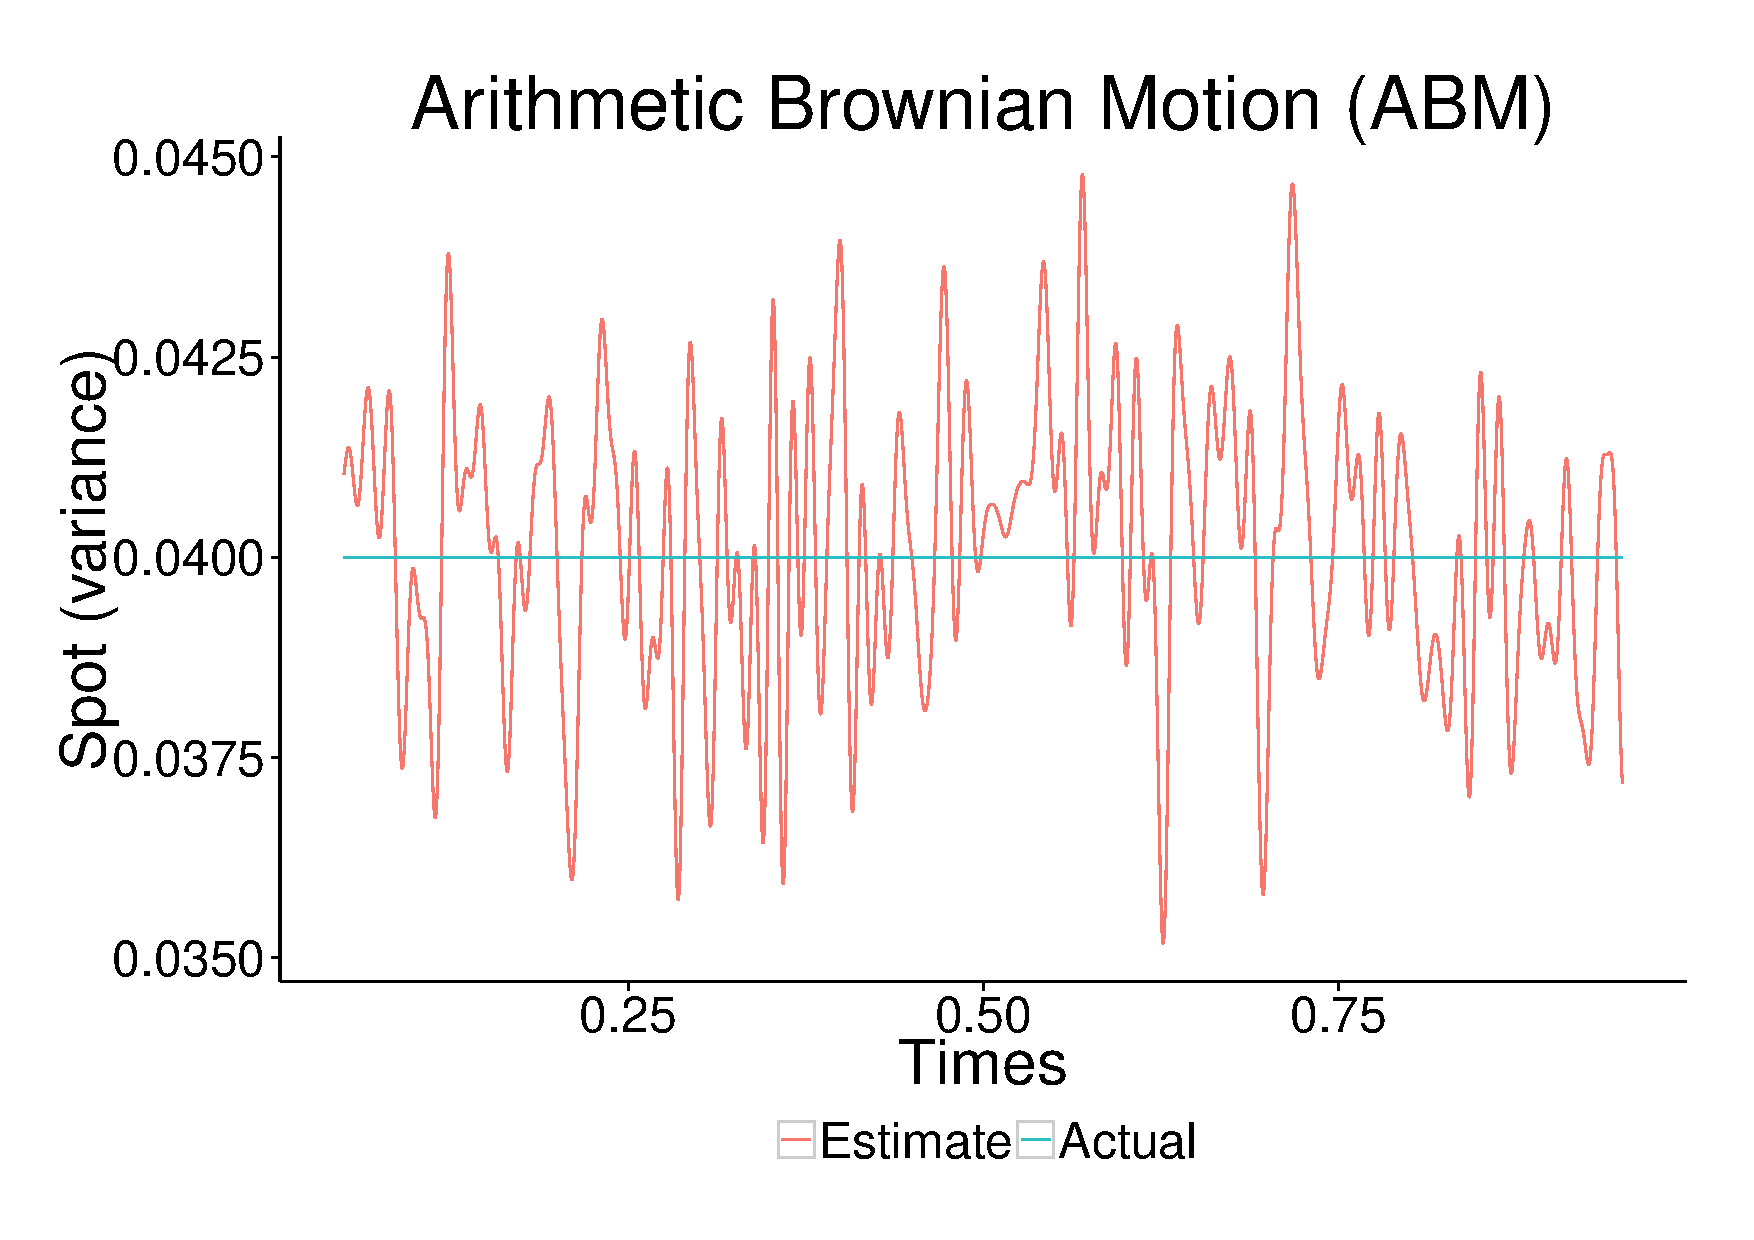
\includegraphics[angle=270,width=0.45\textwidth,totalheight=0.30\textheight]{Simulation/pa.pdf}}}
  \subfloat[GBM]{{ \includegraphics[width=0.45\textwidth]{/home/wale/Dropbox/Research/Paper3/pg.pdf}}}
  \qquad
  \subfloat[OU]{{ \includegraphics[width=0.45\textwidth]{/home/wale/Dropbox/Research/Paper3/po.pdf}}}
  \qquad
  \subfloat[ABM]{{ 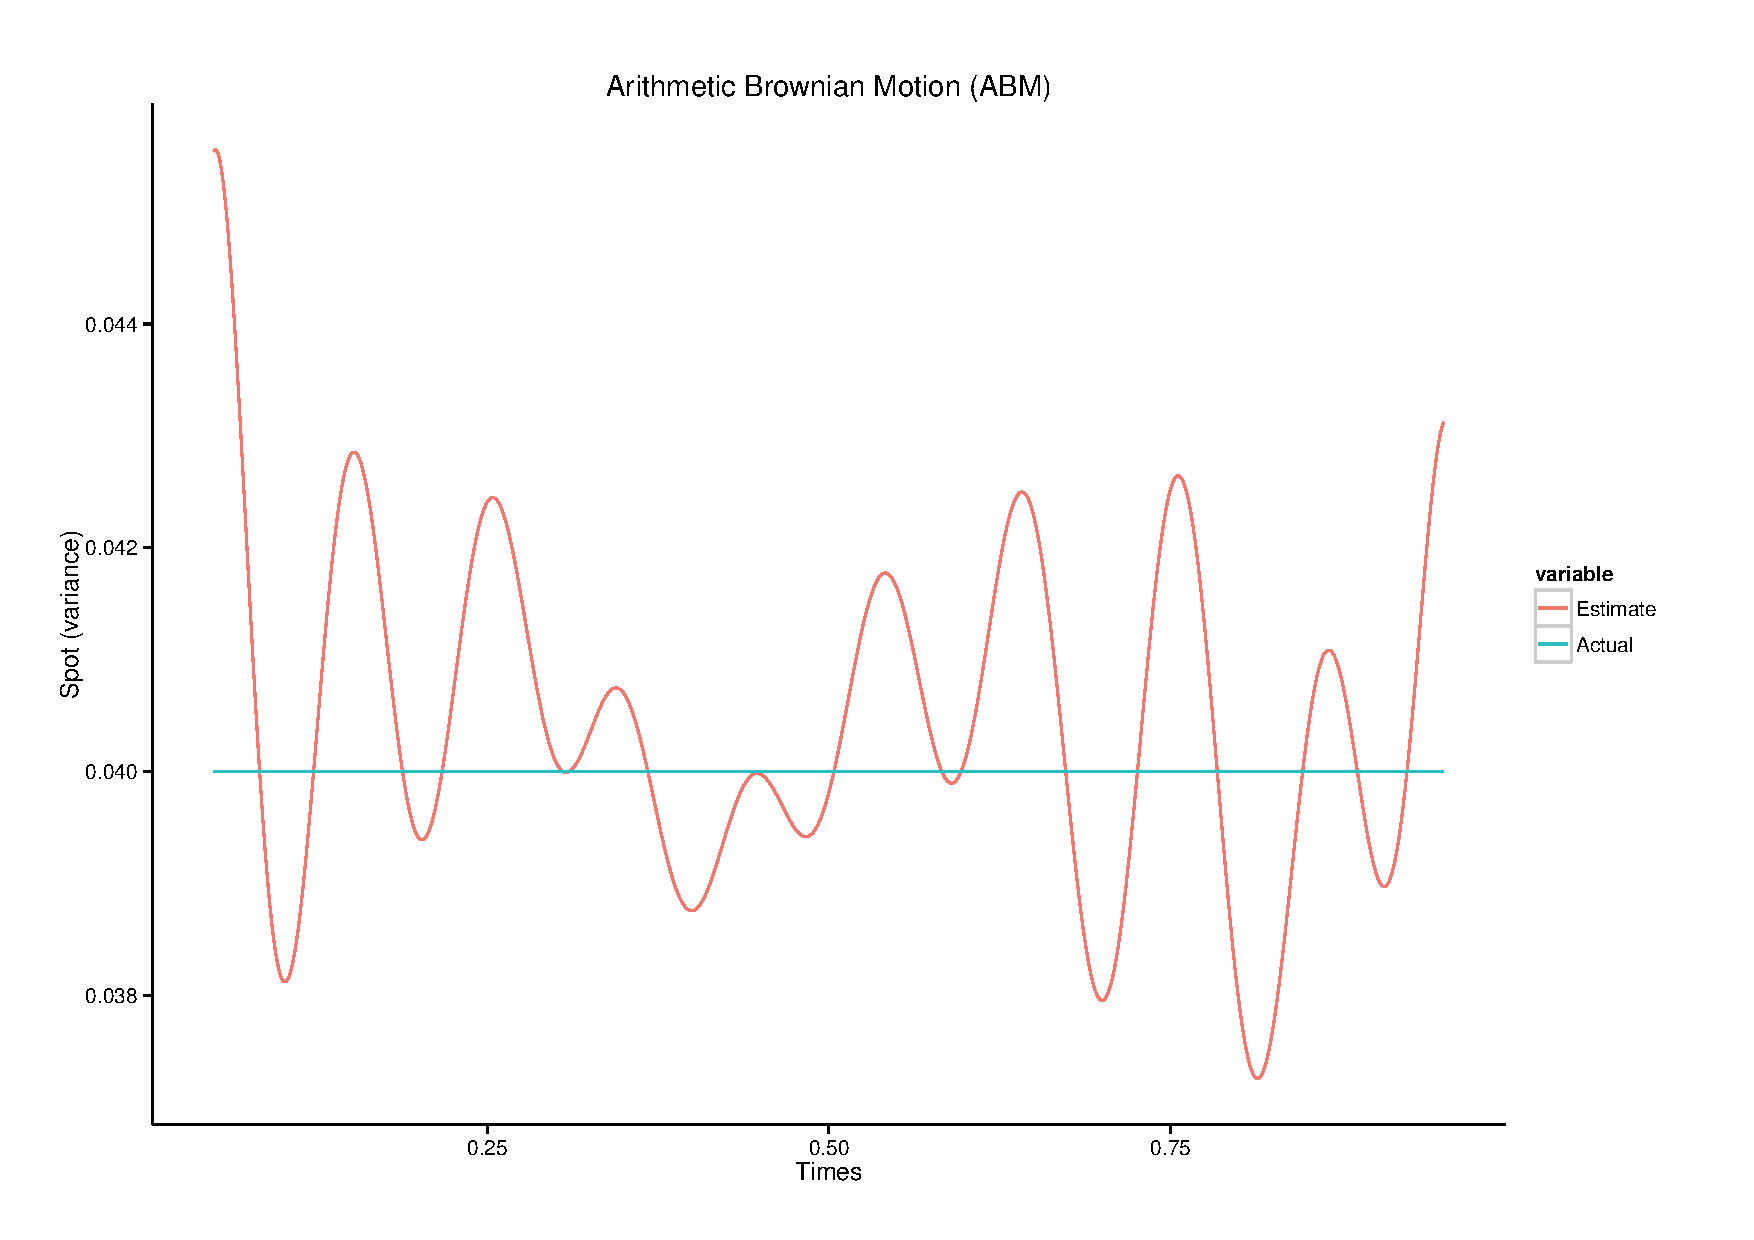
\includegraphics[width=0.45\textwidth]{/home/wale/Dropbox/Research/Paper3/pa.pdf}}}
  \subfloat[CIR]{{ 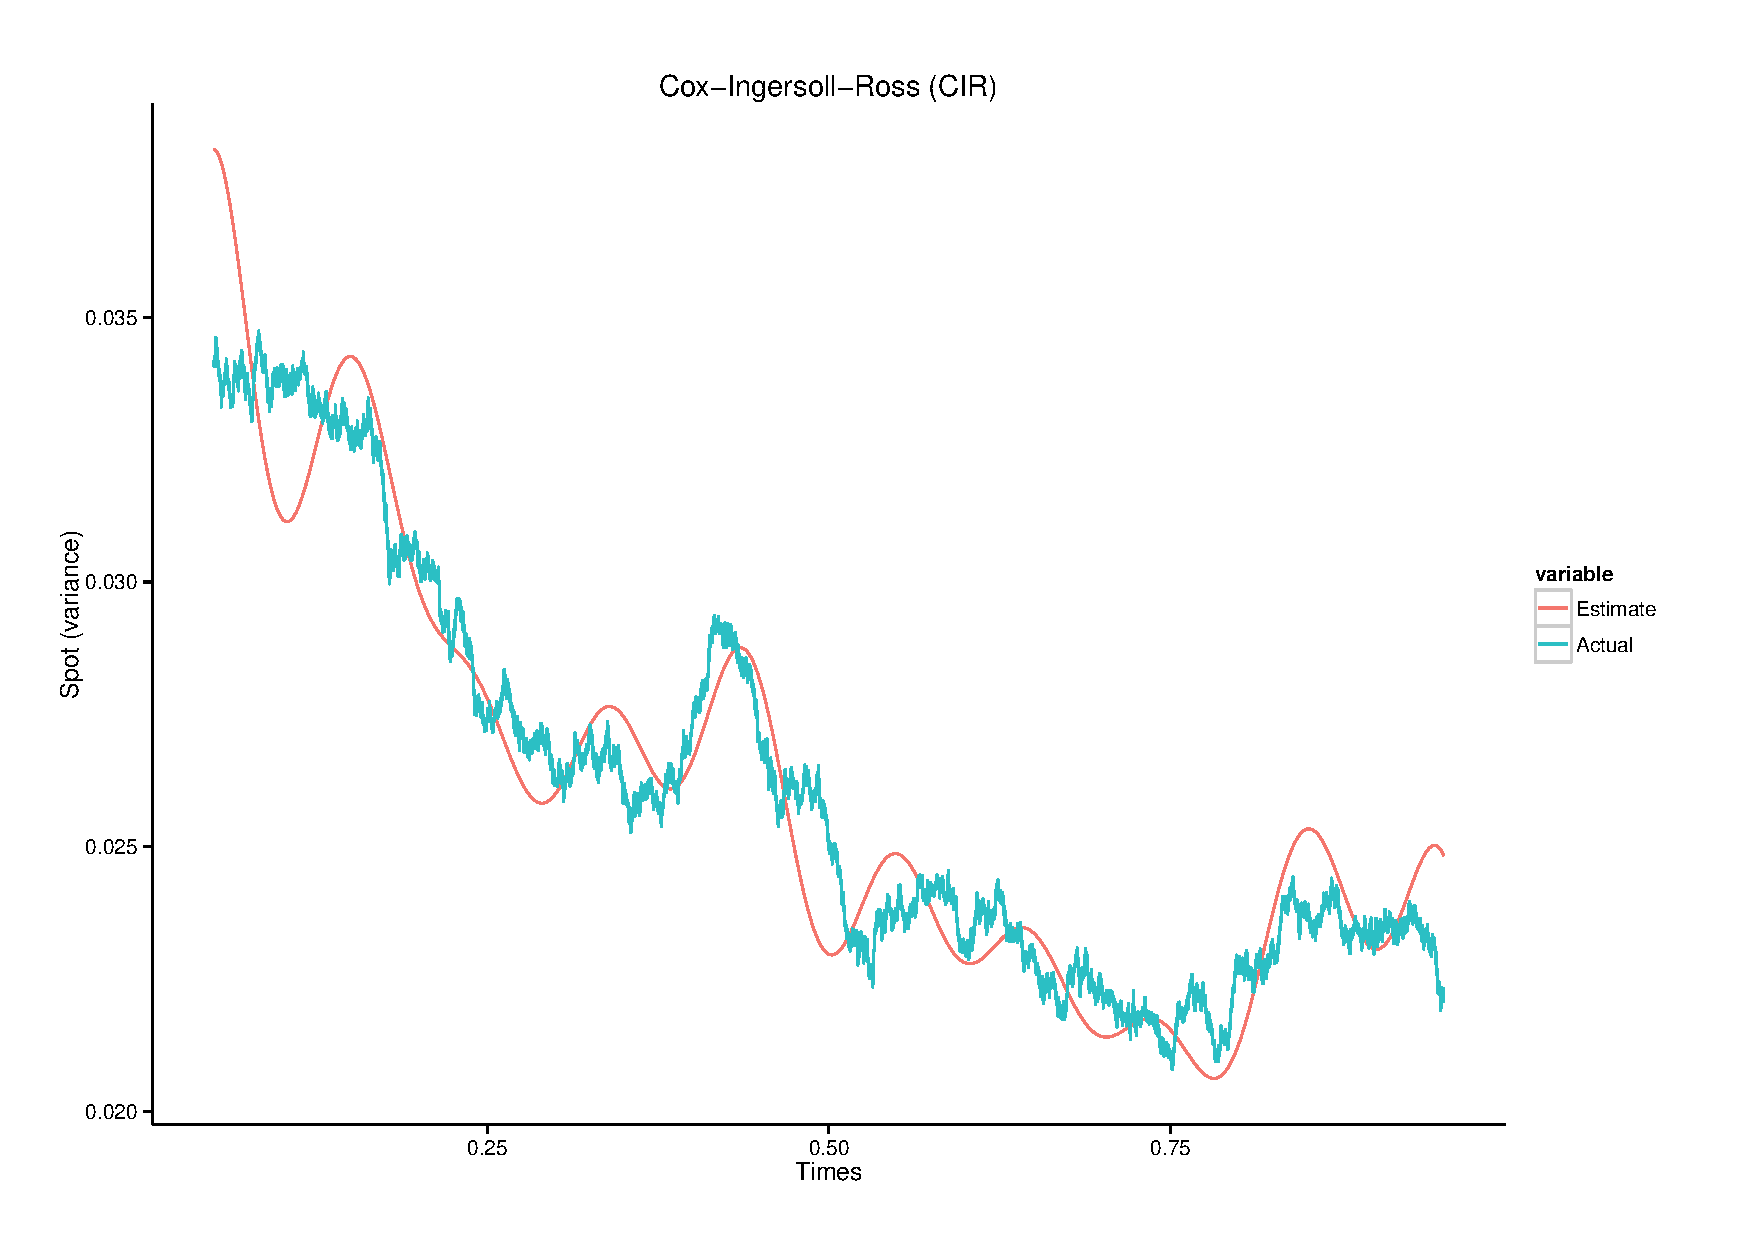
\includegraphics[width=0.45\textwidth]{/home/wale/Dropbox/Research/Paper3/pcir.pdf}}}
    \label{fig:path}
\end{figure}

\begin{landscape}
\begin{table}[ht]
  %\tabcolsep=0.11cm
\begin{threeparttable}
  %\footnotesize
%\centering
  \caption{Mean integrated square error (MISE) of $\svnx$.\label{tab:mise}}
  
\begin{tabular*} {\columnwidth}{@{\extracolsep{\stretch{1}}}*{8}{r}@{}}
    \toprule 
   & \multicolumn{3}{c}{ABM} & &\multicolumn{3}{c}{OU}\\
    \cmidrule{2-4} 
    \cmidrule{5-8} 
\multicolumn{1}{c}{$n$} & \multicolumn{1}{c}{MISE} & \multicolumn{1}{c}{Sq. Bias} & \multicolumn{1}{c}{Var} && \multicolumn{1}{c}{MISE}& \multicolumn{1}{c}{Sq. Bias} & \multicolumn{1}{c}{Var}\\
    \midrule
500 & \num[scientific-notation=true,round-precision=3,round-mode=figures]{ 0.000129690514378747 } & \num[scientific-notation=true,round-precision=3,round-mode=figures]{ 2.86098860978027e-06 } & \num[scientific-notation=true,round-precision=3,round-mode=figures]{ 0.000126829525768967 } & & \num[scientific-notation=true,round-precision=3,round-mode=figures]{ 0.000142657171197515 } & \num[scientific-notation=true,round-precision=3,round-mode=figures]{ 1.19241391058862e-05 } & \num[scientific-notation=true,round-precision=3,round-mode=figures]{ 0.000130733032091629 } \\
5000 &\num[scientific-notation=true,round-precision=3,round-mode=figures]{ 1.41480010731752e-05 } & \num[scientific-notation=true,round-precision=3,round-mode=figures]{ 1.11112511718854e-06 } & \num[scientific-notation=true,round-precision=3,round-mode=figures]{ 1.30368759559867e-05 } & & \num[scientific-notation=true,round-precision=3,round-mode=figures]{ 1.44713297500796e-05 } & \num[scientific-notation=true,round-precision=3,round-mode=figures]{ 1.62292548526195e-06 } & \num[scientific-notation=true,round-precision=3,round-mode=figures]{ 1.28484042648177e-05 } \\ 
50000 &\num[scientific-notation=true,round-precision=3,round-mode=figures]{ 2.32308652636521e-06 } & \num[scientific-notation=true,round-precision=3,round-mode=figures]{ 1.02395100012948e-06 } & \num[scientific-notation=true,round-precision=3,round-mode=figures]{ 1.29913552623573e-06 } & & \num[scientific-notation=true,round-precision=3,round-mode=figures]{ 2.35629081189399e-06 } & \num[scientific-notation=true,round-precision=3,round-mode=figures]{ 1.12403547001524e-06 } & \num[scientific-notation=true,round-precision=3,round-mode=figures]{ 1.23225534187875e-06 } \\
   \midrule
  \end{tabular*}
\end{threeparttable}
\begin{threeparttable}
  %\footnotesize
%\centering
\begin{tabular*} {\columnwidth}{@{\extracolsep{\stretch{1}}}*{8}{r}@{}}
    \midrule
   & \multicolumn{3}{c}{GBM} & &\multicolumn{3}{c}{CIR}\\
    \cmidrule{2-4} 
    \cmidrule{5-8} 
\multicolumn{1}{c}{$n$} & \multicolumn{1}{c}{MISE} & \multicolumn{1}{c}{Sq. Bias} & \multicolumn{1}{c}{Var} && \multicolumn{1}{c}{MISE}& \multicolumn{1}{c}{Sq. Bias} & \multicolumn{1}{c}{Var}\\
    \midrule
500 & \num[scientific-notation=true,round-precision=3,round-mode=figures]{ 0.000217858539705785 } & \num[scientific-notation=true,round-precision=3,round-mode=figures]{ 4.17515036941201e-06 } & \num[scientific-notation=true,round-precision=3,round-mode=figures]{ 0.000213683389336373 } && \num[scientific-notation=true,round-precision=3,round-mode=figures]{ 6.25847666534302e-05 } & \num[scientific-notation=true,round-precision=3,round-mode=figures]{ 8.51220421884097e-07 } & \num[scientific-notation=true,round-precision=3,round-mode=figures]{ 6.17335462315461e-05 } \\ 

5000 & \num[scientific-notation=true,round-precision=3,round-mode=figures]{ 2.32787518909845e-05 } & \num[scientific-notation=true,round-precision=3,round-mode=figures]{ 1.58307630511742e-06 } & \num[scientific-notation=true,round-precision=3,round-mode=figures]{ 2.16956755858671e-05 } && \num[scientific-notation=true,round-precision=3,round-mode=figures]{ 6.82420050132428e-06 } & \num[scientific-notation=true,round-precision=3,round-mode=figures]{ 5.99985785058558e-07 } & \num[scientific-notation=true,round-precision=3,round-mode=figures]{ 6.22421471626572e-06 } \\
50000 & \num[scientific-notation=true,round-precision=3,round-mode=figures]{ 4.6593085666358e-06 } & \num[scientific-notation=true,round-precision=3,round-mode=figures]{ 1.01842335658939e-06 } & \num[scientific-notation=true,round-precision=3,round-mode=figures]{ 3.64088521004641e-06 } && \num[scientific-notation=true,round-precision=3,round-mode=figures]{ 1.45783049273178e-06 } & \num[scientific-notation=true,round-precision=3,round-mode=figures]{ 6.05894054142823e-07 } & \num[scientific-notation=true,round-precision=3,round-mode=figures]{ 8.51936438588961e-07 } \\
    \bottomrule
\end{tabular*}
  \medskip
  \footnotesize
Note: The mean of the integrated square errors are obtained by taking an average over 100 sample paths generated  for each  model/number of observations pair.
\end{threeparttable}
\end{table}

\end{landscape}

From an implementation perspective, using a  B-spline  makes the construction of a \emph{dual}  frame generator a trivial matter. This is a consequence of Theorems 2.2 and 2.7 in \cite{Christensen2006}, which together specify a very simple rule for constructing  dual pairs: Let $a>0$ and $b>0$ denote  translation and modulation parameters, and let   $h$ be a B-spline of order $p$. Define the dilation operator  $\mcal{D}_c$ as follows:
\begin{align}
  \mcal{D}_c f(x) = c^{-1/2}f(x/c).  \label{eq:dilation}
\end{align}
If $0 < ab \le 1/(2 p -1)$ then  $\{\mcal{D}_a h, \mcal{D}_a\tilde{h}\}$, where 
\begin{align}
  \tilde{h}(x) = ab h(x) + 2 a b \sum^{p-1}_{n=1} h(x+n), \qquad \forall x \in \real, 
  \label{eq:gt}
\end{align}
is a pair of  dual Gabor  frame generators. So if we start with a B-spline $h$ then the dual generator will be a finite linear combination of scaled translates of $h$; consequently, the  dual generator will be a spline, with similar regularity properties.  For our simulation, we used a third-order B-spline. Our choice of the third order B-spline is motivated by a desire for a generator with a  Fourier transform that decays like a quadratic polynomial.   Specifically, we set
\begin{align}
  h(x) = \left\{
    \begin{array}{lr}
    x^2/2 & x \in (1,0]\\
  (-2x^2 + 6x - 3)/2 & x \in (2,1]\\
(3-x^2)/2 & x \in (3,2]\\
0 & x \not\in (3,0]
\end{array}\right. ,
  \label{eq:theh}
\end{align}
with  $\tilde{h}$ computed as in \eqref{eq:gt} above.
Our choice of the modulation and translation parameters is rather arbitrary. The only constraint is that $0 < ab \le 1/(2p -1) = 1/5$; from our experimentation with different values, performance seems to be about the same for different choices satisfying the inequality;  we settled on $a = 1/5$ and $b = 1/3$.  Ideally $H_n$, the order of the number of frequency domain shifts, would be selected optimally to minimize MISE while balancing integrated variance and integrated square  bias; we will turn our attention to this problem in future work. For the time being we  set $H_n$ naively equal to 50.

The simulation results indicate that the Gabor frame estimator performs satisfactorily. Figure~\ref{fig:path} displays, for each of the 4 price models (ABM, OU, GBM, and CIR), simulated  spot variance sample paths plotted against spot variance paths produced by the Gabor frame estimator.  A visual inspection shows that the estimator produces a relatively good fit even with the naive selection of $H_n$. This claim is further corroborated by the analysis of the the \mise (MISE), the \isqb, and the \ivar summarized in Table \ref{tab:mise}. 
The figures in the table are arrived at in the following manner: first,  100 price histories are simulated for each observation frequency and  model pair.  So, each history is the result of sampling $n$ price observations from  distribution $F$, where $n$ is the specified observation frequency and $F$ is the distribution implied by the stochastic differential equation. The resulting data is a matrix with 100 rows and $n$ columns.  Each row represents a price history from which integrated quatities may be obatined, and each column indexes an orbservation time. Going down a column, average quantities may be computed. 
For instance, to arrive at the integrated square bias figures, average spot variances were computed for each observation times; the figures were then squared, weighted by $\Delta_n$, and summed up. The integrated mean square error is computed similarly.
 We found that the variance, estimated in the foregoing manner,  is only approximately the difference between the MISE and the integrated square bias.  The reported figures for variance are  in fact the difference between the MISE and the integrated square bias. The discrepancy is rather slight and does not materially change the result. In all 4 model, an inverse relation between MISE, square bias, and variance may be read off from the table. As was established mathematically, we expect MISE to vanish if the number of price observations were made to grow without bound.    
 \subsection{Prices with jumps}
 In Propositions \eqref{pro:finite} and \eqref{pro:infinity}, we demonstrate analytically that $\jvn$ is consistent in term of the \Ltwo distance when prices contain jumps of finite and infinite activity, respectivey. These results, however, do not assert the convergence of the mean integrated squared error of the estimator. Nevertherless, the consistency results lead us to suspect that the MISE of the estimator is also convergent. We investigate this analysis by simulating for price prosesses with jumps:    
\begin{align}
  & X_t = 0.8 +  0.5  t + 0.2  W_t + \sum_{i = 1}^N Y_i,\notag & \text{(ABM + JMP)}\\
  & X_t = 0.8 -\int_0^t 4 X_s \D s + \int^t_0 0.2 \D W_s +  \sum_{i = 1}^N Y_i ,\notag & \text{(OU + JMP)}\\
  & X_t = 0.8 + \int_0^t 0.5 X_s \D s + \int^t_0 0.2 X_s \D W_s + \sum_{i = 1}^N Y_i,\notag & \text{(GBM + JMP)}\\
  & X_t = 0.8 + \int_0^t(0.1 - 0.5 X_s) \D s +\int^t_0  0.2 \sqrt{X_s} \D W_s + \sum_{i = 1}^N Y_i,\notag & \text{(CIR + JMP)}
  \label{}
\end{align}
wher $N$ is a Poisson random variable with intensity $5$ and $Y_i$, $1 \le  i\le N$, is a normal random variable with mean zero and standard deviation 0.4.  

We construct the dual  Gabor frames as in the previous subsection using the  third order B-Spline specified in \eqref{eq:theh}. With the introduction of jumps into the simulation, we found out that better results may be obtained by varying tha parameters $a,b,$ and $H_n$. We settled on $a = 1/7$, $b = 1/25$, and $H_n = 50$. The jump threshold is obtained by setting $u_n = n^{\alpha}$, where $\alpha = -0.45$. The results of the simulations are recorded in Table~\ref{tab:misej}. We also produce a graph of a single observations (paths) in Figure~\ref{fig:pathj}. It is apparent from this simulation study that, eventhough the analytical part of the analysis assumed that volatility is continuous, the estimator \jvn works fine in cases where volatiity is \cadlag. This is the case when we add jumps to the geometric Brownian  and the CIR processes. We defer an analytical study of this more general situation to future work.
\begin{figure}
  \caption{Estimated vs. actual spot volatility of common price models}
  \centering
  %\subfloat[ABM]{{ 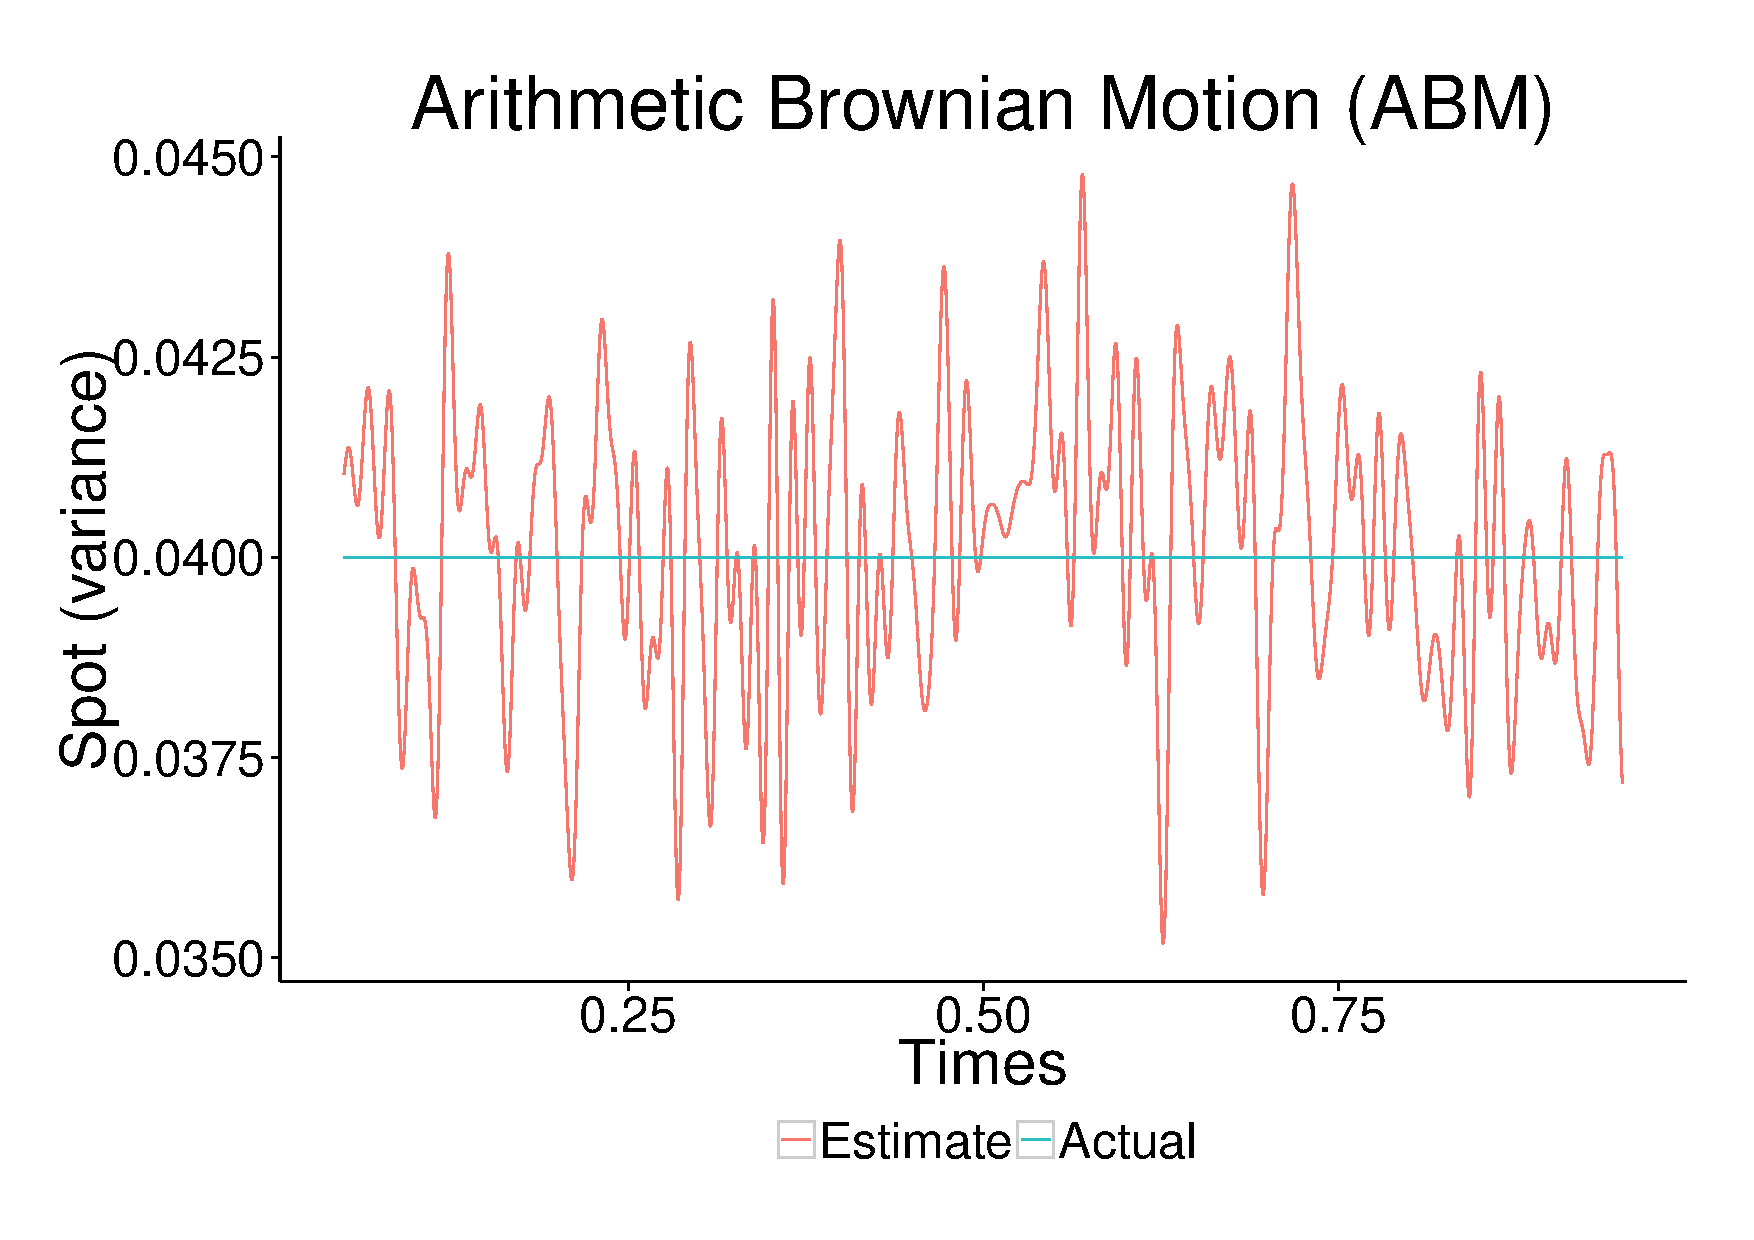
\includegraphics[angle=270,width=0.45\textwidth,totalheight=0.30\textheight]{Simulation/pa.pdf}}}
  \subfloat[GBM + JMP]{{ \includegraphics[width=0.45\textwidth]{/home/wale/Dropbox/Research/Paper3/Simulation/pg.pdf}}}
  \qquad
  \subfloat[OU + JMP]{{ \includegraphics[width=0.45\textwidth]{/home/wale/Dropbox/Research/Paper3/Simulation/po.pdf}}}
\qquad
  \subfloat[ABM]{{ 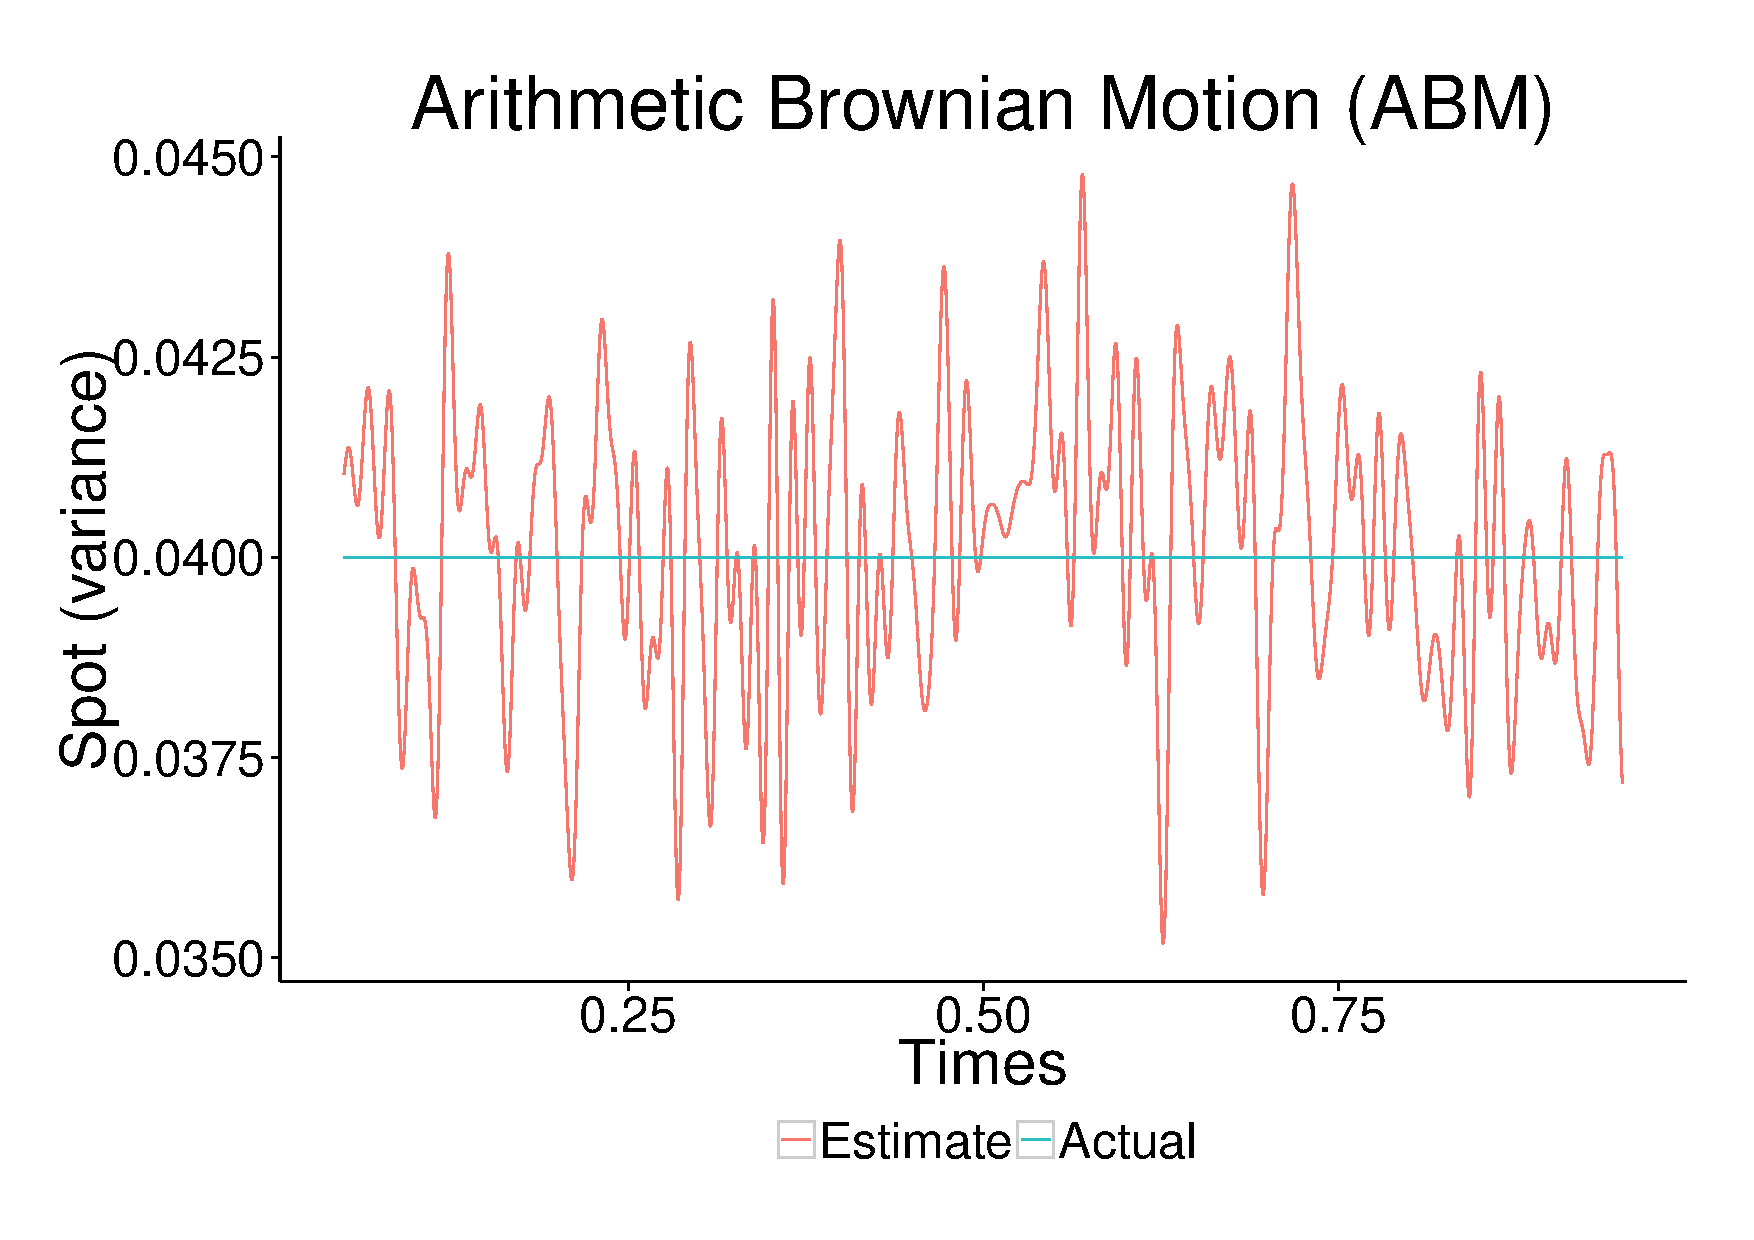
\includegraphics[angle=270,width=0.45\textwidth,totalheight=0.30\textheight]{Simulation/pa.pdf}}}
%  \subfloat[GBM+JUMP]{{ 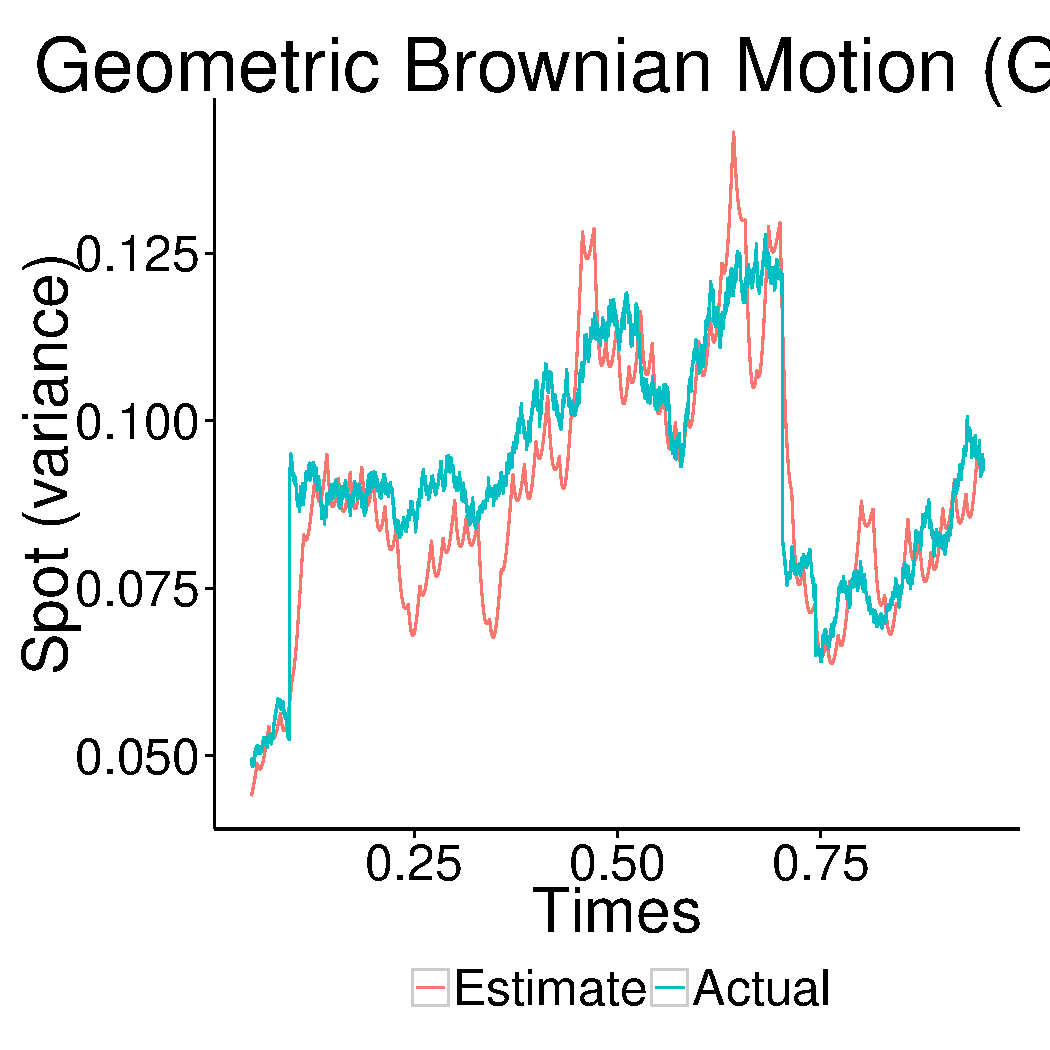
\includegraphics[width=0.45\textwidth]{/home/wale/Dropbox/Research/Paper3/Simulation/bpg.pdf}}}
  \qquad
  \subfloat[CIR+JUMP]{{ 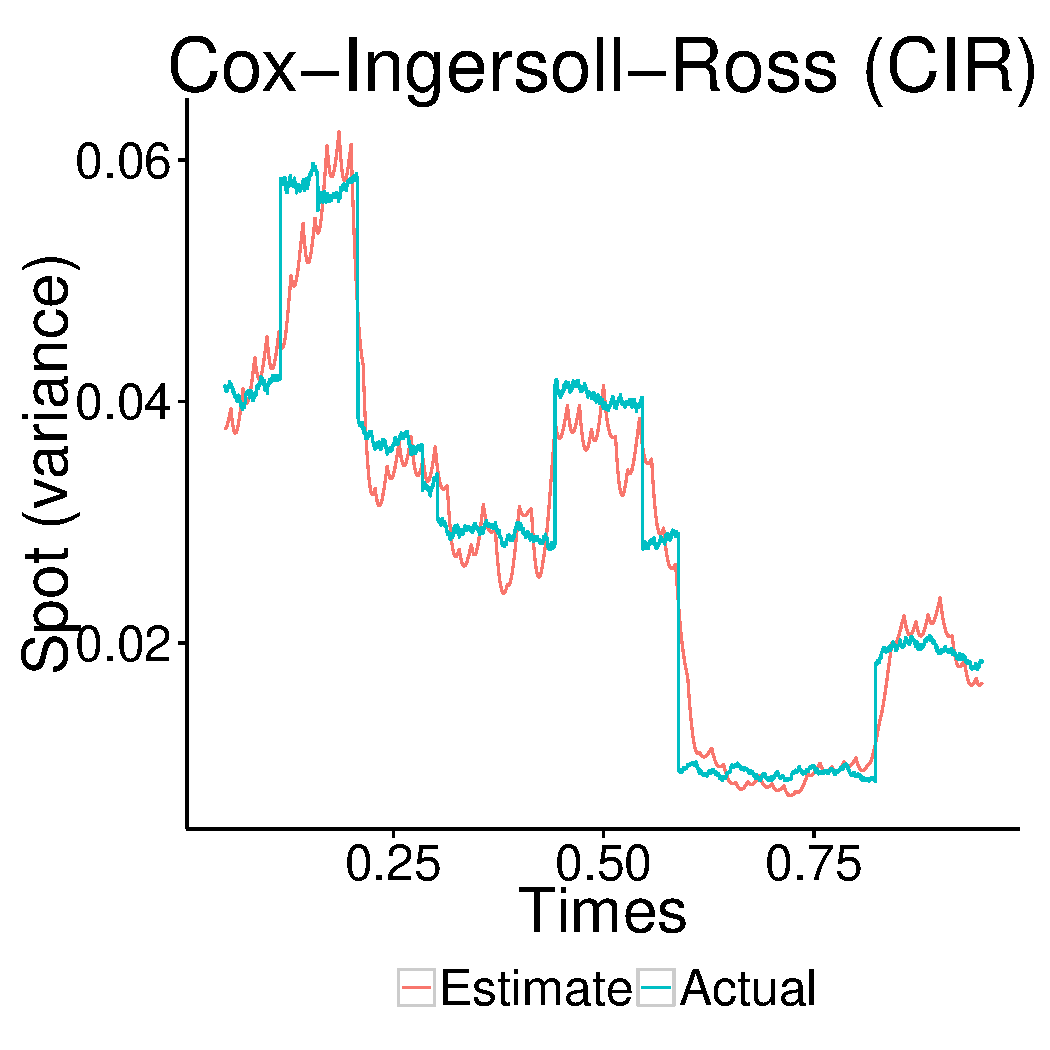
\includegraphics[width=0.45\textwidth]{/home/wale/Dropbox/Research/Paper3/Simulation/bpc.pdf}}}
    \label{fig:path}
\end{figure}

\begin{table}[ht]
  %\tabcolsep=0.11cm
\begin{threeparttable}
  %\footnotesize
%\centering
  \caption{Mean integrated square error (MISE) of the frame-based estimator $\hat{\sigma}_n^2$ for popular price models.\label{tab:mise}}
  
\begin{tabular*} {\columnwidth}{@{\extracolsep{\stretch{1}}}*{8}{r}@{}}
    \toprule 
   & \multicolumn{3}{c}{FP} & &\multicolumn{3}{c}{OU}\\
    \cmidrule{2-4} 
    \cmidrule{5-8} 
\multicolumn{1}{c}{$n$} & \multicolumn{1}{c}{MISE} & \multicolumn{1}{c}{Sq. Bias} & \multicolumn{1}{c}{Var} && \multicolumn{1}{c}{MISE}& \multicolumn{1}{c}{Sq. Bias} & \multicolumn{1}{c}{Var}\\
    \midrule
500 & \num[scientific-notation=true,round-precision=3,round-mode=figures]{ 0.000152943970286857 } & \num[scientific-notation=true,round-precision=3,round-mode=figures]{ 8.95426446735699e-06 } & \num[scientific-notation=true,round-precision=3,round-mode=figures]{ 0.0001439897058195 } && \num[scientific-notation=true,round-precision=3,round-mode=figures]{ 0.0008507085185364 } & \num[scientific-notation=true,round-precision=3,round-mode=figures]{ 0.000130637321821816 } & \num[scientific-notation=true,round-precision=3,round-mode=figures]{ 0.000720071196714584 } \\ 
5000 & \num[scientific-notation=true,round-precision=3,round-mode=figures]{ 2.18676452382767e-05 } & \num[scientific-notation=true,round-precision=3,round-mode=figures]{ 2.27386491244051e-06 } &  \num[scientific-notation=true,round-precision=3,round-mode=figures]{ 1.95937803258361e-05 } && \num[scientific-notation=true,round-precision=3,round-mode=figures]{ 5.47538962275779e-05 } & \num[scientific-notation=true,round-precision=3,round-mode=figures]{ 9.75968033436806e-06 } & \num[scientific-notation=true,round-precision=3,round-mode=figures]{ 4.49942158932098e-05 } \\ 
50000 & \num[scientific-notation=true,round-precision=3,round-mode=figures]{ 2.1312724152077e-06 } & \num[scientific-notation=true,round-precision=3,round-mode=figures]{ 8.9974544209342e-08 } & \num[scientific-notation=true,round-precision=3,round-mode=figures]{ 2.04129787099836e-06 } && \num[scientific-notation=true,round-precision=3,round-mode=figures]{ 6.6114774335773e-06 } & \num[scientific-notation=true,round-precision=3,round-mode=figures]{ 2.64501211826553e-06 } & \num[scientific-notation=true,round-precision=3,round-mode=figures]{ 3.96646531531177e-06 } \\
   \midrule
  \end{tabular*}
\end{threeparttable}
\begin{threeparttable}
  %\footnotesize
%\centering
\begin{tabular*} {\columnwidth}{@{\extracolsep{\stretch{1}}}*{8}{r}@{}}
    \midrule
   & \multicolumn{3}{c}{GBM} & &\multicolumn{3}{c}{CIR}\\
    \cmidrule{2-4} 
    \cmidrule{5-8} 
\multicolumn{1}{c}{$n$} & \multicolumn{1}{c}{MISE} & \multicolumn{1}{c}{Sq. Bias} & \multicolumn{1}{c}{Var} && \multicolumn{1}{c}{MISE}& \multicolumn{1}{c}{Sq. Bias} & \multicolumn{1}{c}{Var}\\
    \midrule


500 & \num[scientific-notation=true,round-precision=3,round-mode=figures]{ 0.00613398704893088 } & \num[scientific-notation=true,round-precision=3,round-mode=figures]{ 0.000870352351606066 } & \num[scientific-notation=true,round-precision=3,round-mode=figures]{ 0.00526363469732481 } && \num[scientific-notation=true,round-precision=3,round-mode=figures]{ 0.000374450452612452 } & \num[scientific-notation=true,round-precision=3,round-mode=figures]{ 0.000231573404584565 } & \num[scientific-notation=true,round-precision=3,round-mode=figures]{ 0.000142877048027886 } \\ 
5000 & \num[scientific-notation=true,round-precision=3,round-mode=figures]{ 0.000342385006317484 } & \num[scientific-notation=true,round-precision=3,round-mode=figures]{ 4.07189648661911e-05 }  &\num[scientific-notation=true,round-precision=3,round-mode=figures]{ 0.000301666041451293 } && \num[scientific-notation=true,round-precision=3,round-mode=figures]{ 1.12423351227354e-05 } & \num[scientific-notation=true,round-precision=3,round-mode=figures]{ 8.2888360643758e-06 } & \num[scientific-notation=true,round-precision=3,round-mode=figures]{ 2.95349905835962e-06 } \\ 
50000 & \num[scientific-notation=true,round-precision=3,round-mode=figures]{ 7.10632627767849e-05 } & \num[scientific-notation=true,round-precision=3,round-mode=figures]{ 6.36155753555274e-06 } & \num[scientific-notation=true,round-precision=3,round-mode=figures]{ 6.47017052412321e-05 } && \num[scientific-notation=true,round-precision=3,round-mode=figures]{ 7.04582898194268e-06 } & \num[scientific-notation=true,round-precision=3,round-mode=figures]{ 5.64425630312442e-06 } & \num[scientific-notation=true,round-precision=3,round-mode=figures]{ 1.40157267881827e-06 } \\
    \bottomrule
\end{tabular*}
  \medskip
  \footnotesize
Note: The mean of the integrated square errors are obtained by taking an average over 50 sample paths generated  for each  model/number of observations pair.
\end{threeparttable}
\end{table}



\section{Volatility estimation: discontinuous prices} 
In this section we specify a global spot volatility estimator for possibly discontinuous \ito semimartingale price processes. That is, for $t \ge 0$,
  \begin{align}
    &X_t = X_0 + \int^t_0 b_s ds + \int^t_0 \sigma_s d W_s  + x  I_{\{\vert x \vert > 1\}} \ast \mu_t  + x  I_{\{\vert x \vert \le  1\}} \ast (\mu - \nu)_t 
  \notag \end{align}
with  $\nu(dt, dx) = F(dx) dt$ for a determinsistic  and constant-in-time $\sigma$-finite measure $F$. We assume $\sigma$ and $b$ satisfy the requirements of Assumption \ref{as:vol}, and we further restrict the \levy system of $X$ as follows:
\begin{ass} \label{as:nu}
  \mbox{}
 %   \item  There is a sequence of stopping times $T_m \uparrow \infty$, a.s., and a sequence $\{F^m\}$ of deterministic $\sigma$-finite measures  on the real line satisfying 
  %    \begin{align} 
   %     \int_\real (x^2 \wedge \vert x \vert)  F^m(dx) <\infty\end{align}
   %     such that $\sup_{t \wedge T_m} F_t (B) \le F^m(B)$ almost surely for all Borel sets $B$.
    %\item $x^2  \ast \nu_t = \int_0^t \int_\real x^2 F_t(dx) dt < \infty$,
  The \levy measure $F$ satisfies the following condition
  $(x^2I_{\{\vert x \vert \le u\}})\ast \nu_t = \int_0^t \int_{-u}^{u} x^2 F( \D x) \D t = O(u)$ as $u \to 0$.
\end{ass}
\begin{remark}
% The first requirement implies the existence of $T_m \uparrow \infty$, a.s., such that $X_{t \wedge T_m} - X_0$ has square integrable small jumps and large jumps  of integrable variataion for each $m$.  The requirement is met by price processes with locally bounded jumps. %It also implies that the jumps of $X$  in excess of one are of locally integrable varaition, so that $X$ is a special martingale.

  The  requirement  is satisfied if $F$ is absolutely continuous with bounded density $f$, as is the case with the Gaussian distribution; more generally, it is satisfied  if  $f(x) = O(x^{-2})$ as $x \to 0$; these include the \levy$(\gamma, \delta)$ distribution with density 
  \begin{align}
    f(x) = (\gamma/2 \pi)^{1/2} (x - \delta)^{-3/2} \exp(-\gamma/ 2(x - \delta)),  \qquad x \in \real, \notag
    \label{}
  \end{align}
  and the Cauchy$(\gamma, \delta)$ distribution with density
  \begin{align}
    f(x) = (\gamma/\pi) (\gamma^2 + (x - \delta)^2)^{-1}, \qquad x > \delta.\notag
    \label{}
  \end{align}

  We also remark that for general semimartingales $(x^2 \wedge 1)\ast  \nu_t$ is increasing and locally integrable. By the \levy assumption, we simply have that  $(x^2 \wedge 1) *  \nu$ is finite. In addition, it is a consequence of the \levy assumption that the price process has no fixed time of discontinuity \citep[II.4.3]{Jacod2003}. Hence, by \ito's integration by parts formula 
  \begin{align}
    \e((x^2\wedge 1)\ast \mu_t) = t(x^2 \wedge 1) *  \nu = O(t), \qquad t \ge 0. \label{eq:secmo}
  \end{align}
\end{remark}

\begin{comment}
 Let $\tau: \real \to \real$ be bounded and satisfy $\tau(x) = x$ in a neighborhood of 0.  Let $\iota$ be the identity  function on the real line, i.e.  $\iota(x) = x$ for $x \in \real$. The price process $X$ admits the following  representation:
\begin{align}
  X_t & = X_0 + \int_0^t b_s \D s + \int_0^t \sigma_s \D W_s +  \tau(x)\ast (\pme  - \nu)_t  + (\iota - \tau)(x)\ast \pme_t ,   
  \label{eq:generalsemimartingale}
\end{align}
for $t \ge 0$  where  \sbm is a standard Brownian motion;  $X_0$ is either known or observable at time 0;  both $b$ and $\sigma$ are adapted; $b$ is \cadlag, and $\sigma$ is continuous;  \pme is a Poisson random measure on $\real_+ \times \real$ with intensity $\nu$, where $\nu$ is a  $\sigma$-finite L\'evy  measure on $\real_+ \times \real$. Note that because $\mu$ is a Poisson measure, if $A$ and $B$ are disjoint Borel sets on $\real_+ \times \real$, then the random measures $\mu(A)$ and $\mu(B)$ are Poisson distributed, independent, and  and have intensity, $\nu(A)$ and $\nu(B)$, respectively. Moreover, because of the \levy assumption on $\nu$, it is the case that $\nu$ does not charge 0 and 
\begin{align}
  (x^2 \wedge 1) \ast\nu_t < \infty, \qquad t \in [0,1],\notag
  \label{}
\end{align}
where $a \wedge b$, with  $a,b \in \real$, denotes the minimum of $a$ and $b$. The  notation $``\ast"$ denotes integration with respect to a random measure. So that 
\begin{align}
  &J_{t}^l :=  \tau\ast (\pme  - \nu)_t = \int_0^t\int_\real \tau(x) [\pme(\D s, \D x)   -  \nu(\D s,\D x)], \notag\\
  & J_{t}^s:= (\iota - \tau)\ast \pme_t = \int_0^t\int_\real [\iota(x) - \tau(x)] \pme(\D s, \D x), \notag
  \label{}
\end{align}
for $t \ge 0$. Both  $J^l$ and $J^s$ are purely discontinuous in the sense that they are orthogonal to all continuous semimartingales. $J^s$ accounts for  small jumps; it is a square-integrable martingale with possibly infinite activity. $J^l$ accounts for large jumps, i.e. jumps with magnitude exceeding the bound on $\tau$; it neccessarily has finite activity so it is a process with finite variation. In the sequel, we will specify $\tau$ as follows:
\begin{align}
  \tau(x) = xI_{\{\vert x \vert \le 1\}}, \qquad x \in \real. \notag
  \label{}
\end{align}
\end{comment}
As in the preceeding section, we observe a realization of the price process at $n + 1$ equidistant points $t_i$,  $i = 0, 1, \cdots, n$. The observation interval is normalized to \domain with  no loss of generality.  The estimator proposed in the previous section, where there is no jump activity, will not do here. It is inconsistent on account of the presence of jumps; its quality deteriorates as a function of how active the jumps of $X$ are. We will counter this phenomenon with a modified spot variance estimator, but first we introduce the following notation. Let $\dx$ denote $X_{t_{i+1}} - X_{t_i}$ for $i = 0, 1,\cdots, n-1$, and let $u_n$  be a positive decreasing sequence such that 
\begin{align}
  u_n  = O(\Delta_n^\beta), \text{ where }\quad 0< \beta < 1.  
  \label{}
\end{align}
 We specify the jump-robust global estimator of  spot volatility as follows: 
\begin{align}
  \label{eq:jumpvolestimator}
  &\jvn(t) := \sum_{(h,k) \in \Theta_n} \anhk\;g_{h,k}(t), \qquad \forall t \in [0,1], \text{ where}\\
  &\anhk := \sum_{i =0}^{n-1} \btghki (\dx)^2 \indx,
\end{align}
where $\{\ghk, \tghk\}$ is a pair of dual Gabor frames constructed as in Lemma \eqref{le:gabor}; $\Theta_n$ retains its meaning from \eqref{eq:theta}; and \indx is one if $(\dx)^2$ is less than or equal to  $u_n$ and zero otherwise.  


There are obvious similarities between \svnx, defined at  \eqref{eq:contvolestimator},  and \jvn with the key difference being that \jvn discards realized squared increments over intervals that likely contain jumps; $u_n$ determines the threshold for what is included in the computation and what is not. This determination becomes more accurate as the observation interval becomes infinitessimally small. Clearly it makes sense to use \svnx if we have reason to believe that the price process is not subject to jumps; \svnx will always employ   all available data and therefore may be assumed to produce more accurate results.  



\section{Extensions}
\subsection{Estimating the spot co-volatility matrix}
We propose the following extension to \svn from Chapter 1 to a multivariate setting. Let $\{X\}_{t \ge 0}$ be a $d$-dimensional vector of log-prices satisfying the stochastic integral equation:
\begin{align}
  X_t = X_0 + \int^t_0 \mu(t, X_s) \D s + \int^t_0 \sigma(t) \D W_s, \qquad  t \ge 0,\notag
  \label{}
\end{align}
where $\{W_s\}_{t \ge 0}$ is an $m$-dimensional standard Brownian motion; $\mu$ is  $\real^d$-valued, continuous, and locally bounded in both variables; $\sigma$ is $\real^d \times \real^m$-valued, continuous and locally bounded in time.   Let 
\begin{align}
  \Sigma (t) := \sigma(t)\sigma'(t), \qquad t \ge  0\notag
  \label{}
\end{align}
where $\sigma'(t)$ is the transpose of $\sigma(t)$. Our aim is to obtain an estimate for $\Sigma$ on the basis of $n$ discretely and synchronously  observed price vectors $\{X_1,\cdots,X_n\}$ in some fixed time interval $[0,T]$, where $T < \infty$. With very little loss of generality we assume that the prices are observed at equidistant intervals given by 
\begin{align}
\Delta_n : = T/n.
\end{align}
Let $\{g_{h,k}, \tghk\}_{h,k \in \ints}$ be a pair of dual Gabor frames generated as in Lemma \eqref{le:gabor}, and $\Theta_n := \{(h,k) \in \ints^2 : |h| \le H_n \text{ and }|k| \le K_0\}$ with $H_n$ an increasing sequence $n$ and $K_0= \lceil (T + |s| + |r|)/b \rceil$. 
We propose to estimate the spot co-volatility matrix in $[0,T]$ using $\hat{\Sigma}_n$ defined component-wise for $1 \le u,v \le d$ as follows:
\begin{align}
  &\Svn^{u,v}(t) = \sum_{(h,k) \in \Theta_n} \cnhk^{u,v}\;g_{h,k}(t), \text{ where}\label{eq:Sigma}\\
  &\cnhk^{u,v} = \sum_{i =0}^{n-1} \btghki (X_u(t_{i+1}) - X_u(t_i))(X_v(t_{i+1}) - X_v(t_i)).
  \label{}
\end{align}
We conjecture that \Svn is consistent for $\Sigma$ and that it converges in the mean integrated error sense at the same rate of convergence as \svn (more precisely, the same order of convergence. So actual rate modulo a constant factor which we conjecture to be equal to the number $m$ of driving Brownian motions). A rigorous proof of this conjecture will be given and further substantiated with simulations.

\begin{comment}
\section{Conclusion} \label{sec:conclusion}
We proposed an estimator for the spot volatility function using Gabor frame methods. We showed that the estimator converges in a MISE sense and obtained an explicit convergence rate.  The evidence for the validity of the proposed estimator will be further reinforced in a simulation study. We will also take the estimator to task using data from the Forex and bond market. 
\end{comment}
%\appendix
\section{Appendix}
%  \section{Proofs}\label{ap:proof}

\begin{lem} \label{lem:modtg}
  Let the dual Gabor frame generator $\tilde{g}$ be constructed as in \eqref{eq:dualg}. If $\modc{g}{\delta}$ denotes the modulus of continuity of $g$, i.e. $\modc{g}{\delta} := \sup \{|g(t) - g(t')| : t,t' \in \real \text{ and } |t -t'| < \delta\}$,  then   
  \begin{align}
    \modc{\tilde{g}_{j,k}}{\delta} \le C \modc{g}{\delta} \qquad  \hkints\notag,
    \label{}
  \end{align}
  where $C$ is a positive constant.
\end{lem}
\begin{comment}
  \begin{proof}
   $G$ is bounded away from zero. To see this, note that since $g$ has support in  $[r,s]$, the series on the left hand side of \eqref{eq:capg} has finitely many terms for each $t$.  In addition, it is straight forward to verify that $G(t) = G(t+b)$ for all $t$; so,  $G$ is periodic with period $b$. It is also clear that because $g$ is continuous, so is $G$. It follows that $G$ attains its min and max on any interval of length $b$. Let $I_b := [(s+r -b)/2, (s+r +b)/2]$, then
  \begin{align}
    \min_{t\in\real} G(t) &=  \min_{t \in I_b} G(t) \notag\\
    & \ge \min_{t \in I_b}\vert g(t)\vert^2/a.\notag
    \label{}
  \end{align}  
  Because $g$ is continuous and $g$ doesn't vanish in $(r,s)$, we conclude that $G_*:=\min_{t \in \real}G(t) > 0$. It is also straight forward that $G^* := \max_{t \in \real}G(t) < \infty$. Now, let $t, t' \in \real$ such that $\vert t - t' \vert \le \delta$, then 
  \begin{align}
    \vert \tg(t) - \tg(t')\vert & = \vert (G(t)G(t'))^{-1}(g(t)G(t') - g(t')G(t))\vert  \notag\\
    & \le (G_*^{-2})\{\vert g(t)\vert \vert G(t) - G(t') \vert + \vert G(t)\vert \vert g(t) - g(t')\vert\}. 
    \label{eq:difftg}
  \end{align}
Let $\tau := r +  (t \bmod {b})$, and $\tau':=r + (t' \bmod{b})$. It is straight forward to verify that if  $\vert \tau - \tau' \vert \le \delta$, then
\begin{align}
  \vert G(t) - G(t') \vert & \le  \sum_{j = 0}^{\lfloor (s + r)/b \rfloor} \vert g(\tau + j b)^2 - g(\tau' + j b)^2\vert\notag\\
  & \le \sum_{j = 0}^{\lfloor (s + r)/b \rfloor} \vert g(\tau + j b) - g(\tau' + j b) \vert \vert g(\tau + j b) + g(\tau' + j b)\vert\notag\\
  & \le 2 \lceil (s + r)/b\rceil g^*\omega_g(\delta),
  \label{}
\end{align}
where $g^* := \max_{t \in \real} \vert g(t)\vert $. On the other hand, if $\vert \tau - \tau'\vert > \delta$, then 
\begin{align}
  &\vert G(t) - G(t') \vert \notag \\
  &\quad \le \vert g(\tau')^2 - g(r)^2\vert +   \vert g(s)^2 - g(\tau + c)^2 \vert\notag \\
  &\qquad +\sum_{j = 1}^{\lfloor (s + r)/b \rfloor} \{\vert g(\tau + (j-1) b)^2 - g(\tau' + j b)^2\vert\}.  \notag
  \label{}
\end{align}
where $c = \lfloor (s + r)/b \rfloor b $. It follows as above that 
\begin{align}
\vert G(t) - G(t') \vert \le 2 (\lceil (s + r)/b\rceil +1)g^*\omega_g(\delta, T).
\end{align}
Returning to \eqref{eq:difftg}, we see that
\begin{align}
  \vert \tg(t) - \tg(t')\vert \le C_{\tg} \omega_g(\delta),\notag
  \label{}
\end{align}
where $C_{\tg} = G_*^2(2 (\lceil (s + r)/b\rceil +1)(g^*)^2 + G^*)$. Now let \hkints, then
\begin{align}
  \vert \tghk(t) - \tghk(t')\vert & = \vert e^{\i h a t} (\tg(t - kb) -\tg(t'-kb) \vert\notag\\
  &\le \vert (\tg(t - kb) -\tg(t'-kb) \vert \le C_{\tg} \omega_g(\delta).
  \label{}
\end{align}
The last inequality follows because translating a function leaves its modulus of continuity unchanged.\\
\end{proof}
\end{comment}
  \begin{proof}
   $G$ is bounded away from zero. To see this, note that since $g$ has support in  $[r,s]$, the series on the left hand side of \eqref{eq:capg} has finitely many terms for each $t$.  In addition, it is straight forward to verify that $G(t) = G(t+b)$ for all $t$; so,  $G$ is periodic with period $b$. It is also clear that because $g$ is continuous, so is $G$. It follows that $G$ attains its min and max on any interval of length $b$. Let $I_b$ denote the interval $[(s+r -b)/2, (s+r +b)/2]$, then
  \begin{align}
    \min_{t\in\real} G(t) &=  \min_{t \in I_b} G(t) \notag\\
    & \ge  a^{-1}\min_{t \in I_b}\vert g(t)\vert^2.\notag
    \label{}
  \end{align}  
  Because $g$ is continuous and $g$ doesn't vanish in $(r,s)$, we conclude that $G_*:=\min_{t \in \real}G(t) > 0$. It is also straight forward that $G^* := \max_{t \in \real}G(t) < \infty$. Now, let $t, t' \in \real$, $ t > t'$,  such that $\vert t - t' \vert \le \delta$, then 
  \begin{align}
     \vert \tg(t) - \tg(t')\vert & = \vert (G(t)G(t'))^{-1}(g(t)G(t') - g(t')G(t))\vert  \notag\\
    & \le (G_*^{-2})\{\vert g(t)\vert \vert G(t) - G(t') \vert + \vert G(t)\vert \vert g(t) - g(t')\vert\}. 
    \label{eq:difftg}
  \end{align}
For a real number  $x$, denote $\lfloor x \rfloor$  the largest integer less than or equal to $x$ and $\lceil x \rceil$  the smallest integer that is greater  than or equal to $x$. Now,
Let $A$ denote the set of integers $i$ such that $r < t - ib < s$. By definition of $g$, $g(t - j b) = 0$, whenever $j \not\in A$. Since $b > 0$, $A$ contains at most $\lceil( 1 + \vert s \vert + \vert r \vert)/b \rceil$ number of elements.  Let $\tau := \min \{t - ib: i \in A\}$, i.e. $\tau$ is the smallest $t - ib$ such that $i \in A$. Because $A$ contains at most a finite number of elements, there exists an integer $k$ such that $\tau = t - kb$. Set $\tau' := t'-kb$.   
  
   It is straight forward to verify that  $\vert \tau - \tau' \vert \le \delta$ and 
\begin{align}
a  \vert G(t) - G(t') \vert & \le  \sum_{j = 0}^{\lceil ( 1 + \vert s \vert  +\vert r \vert )/b \rceil} \vert g(\tau + j b)^2 - g(\tau' + j b)^2\vert\notag\\
  & \le \sum_{j = 0}^{\lceil (1 + \vert s \vert  +\vert r\vert )/b \rceil} \vert g(\tau + j b) - g(\tau' + j b) \vert \vert g(\tau + j b) + g(\tau' + j b)\vert\notag\\
  & \le 2 \lceil (1 + \vert s \vert  + \vert r \vert)/b\rceil g^*\modc{g}{\delta},
  \label{}
\end{align}
where $g^* := \max_{t \in \real} \vert g(t)\vert $.
Returning to \eqref{eq:difftg}, we see that
\begin{align}
  \vert \tg(t) - \tg(t')\vert \le C_{\tg} \modc{g}{\delta},\notag
  \label{}
\end{align}
where $C_{\tg} = G_*^2(2a (\lceil ( 1 + \vert s \vert  +\vert r\vert)/b\rceil)(g^*)^2 + G^*)$. Now let \hkints, then
\begin{align}
  \vert \tghk(t) - \tghk(t')\vert & = \vert \mathrm{e}^{2 \pi \i h a t} (\tg(t - kb) -\tg(t'-kb)) \vert\notag\\
  &\le \vert \tg(t - kb) -\tg(t'-kb) \vert \le C_{\tg} \modc{g}{\delta}.
  \label{}
\end{align}
The last inequality follows because translating a function leaves its modulus of continuity unchanged.\\
\end{proof}




\begin{comment}
Next, we provide a proof of Proposition \eqref{pr:consistency}. \\\\
\begin{proof}
  We begin with $B^2_n$, the bias component of the integrated mean square error. Using \ito's product formula \citep[p. 257]{Applebaum2009}, we may express, using \ito's isometry theorem, the average deviation at time $t$ as follows:
\begin{align}
  &\e[\svn(t) - \bsv(t)] = B_{1,n}(t) + B_{2,n}(t) + B_{3,n}(t), \notag
\end{align}
where
\begin{align}
  &B_{1,n}(t) :=  \sumt g_{h,k}(t) \left\{\sum_{i=0}^{n-1} \btghki \int_{t_i}^{t_{i+1}}\sigma^2(s) \D s -\chk\right\}, \notag\\
  &B_{2,n}(t) := 2 \sumt g_{h,k}(t)\left\{ \sum_{i=0}^{n-1} \btghki \e\left[\int_{t_i}^{t_{i+1}}(X_s - X_{t_i}) \mu(s,X_s) \D s\right] \right\}, \notag\\
  &B_{3,n}(t) := - \sum_{\substack{(j,k) \not\in \Theta_n }}g_{h,k}(t)\chk. 
  \label{}
\end{align}
The first two components, $B_{1,n}(t)$ and  $B_{2,n}(t)$, result from the fact that   $X$ is being observed discretely; whereas  $B_{3,n}$ results because only a finite number of the frame elements are being used in the approximation. We refer to Theorem 4.1 in  \cite{Zhang2008} for an estimate of  $B_{3,n}$:
\begin{align}
  B_{3,n} = O(\omega_{\bsv}(1/H_n)\log H_n)\notag.
  \label{}
\end{align}
So, the smoother the volatility coefficient the smaller the number of frame elements needed to obtain a decent approximation. We obtain a bound on $B_{1,n}$  by noting that 
\begin{align}
 \sum_{i=0}^{n-1} \btghki\int_{t_i}^{t_{i+1}}\sigma^2(s) \D s -\chk\notag
  & = \sum_{i=0}^{n-1}\int_{t_i}^{t_{i+1}}\sigma^2(s)\{\btghki - \btghks\} \D s\notag \\
  &\le C_\beta\omega_{\tghk} (\Delta_n), \notag
  \label{}
\end{align}
where  $C_\beta = \int^T_0 \sigma^2(s) \D s < \infty$. It follows from Lemma \eqref{lem:modtg} that  
\begin{align}
  B_{1,n}(t) \le C_B H_n\omega_{g}(\Delta_n)\notag 
  %\label{in:b1}
\end{align}
with $C_B = 2(2K_0 + 1)g^*\tg^* C_\beta C_{\tg}$. 
Next, we estimate $B_{2,n} (t)$. Note that
\begin{align}
  X_s - X_{t_i} = \int_{t_i}^s \mu(u,X_u) \D u + \int^s_{t_i} \sigma(u)\D W_u. \notag
  \label{}
\end{align}
So, we may write
\begin{align}
  &\e\left[\int_{t_i}^{t_{i+1}}(X_s - X_{t_i}) \mu(s,X_s) \D s\right]\notag\\
  &\quad = \e\left[\int_{t_i}^{t_{i+1}}\left( \int_{t_i}^s \mu(u,X_u) \D u\right)\mu(s,X_s) \D s\right] \notag \\
  &\qquad + \e\left[\int_{t_i}^{t_{i+1}}\left( \int_{t_i}^s \sigma(u) \D W_u\right)\mu(s,X_s) \D s\right]\notag \\
  &\quad =: \beta_{2,i} + \beta_{3,i}. \notag
\end{align}
By Fubinni's theorem,  the Cauchy-Schwarz inequality,  \ito's isometry theorem, and the linear growth condition on the drift, we have
\begin{align}
  \beta_{3,i} &\le C_T\int_{t_i}^{t_{i+1}}\left( \int_{t_i}^s \sigma^2(u) \D u\right)^{1/2}\e[(1+\vert X_s\vert)^2]^{1/2} \D s\notag\\
& \le C_3 \Delta_n^{3/2}.
  \label{}
\end{align}
Similarly, it may be verified that $\beta_{2,i} \le C_2 \Delta_n^2$. Now we may write
\begin{align}
  B_{2,n}(t) &\le \Delta_n^{1/2}\sumt g_{h,k}(t)\left\{ \sum_{i=0}^{n-1} \btghki C_4 \Delta_n \right\} \notag \\
  & \le ( (2K_0+1)C_4 g^*\tg^* T) (2H_n + 1)\Delta^{1/2}_n\notag\\
  & = O(H_n \Delta^{1/2}_n).
  \label{}
\end{align}
Thus the square bias is bounded as follows:
\begin{align}
  B^2_n &= \int_R (B_{1,n}(t) + B_{2,n}(t)+  B_{3,n}(t))^2 \lambda(t) \D t \notag\\
  &= O(H_n^2 \Delta_n + H^2_n\omega^2_g(\Delta_n)  + \omega^2_{\bsv}(1/H_n)\log^2H_n).
  \label{}
\end{align}
Next, we obtain a  bound for the variance term $V_n$. Recall from \eqref{eq:ivar} that
\begin{align}
V_n :=  \int_\real \e[\{\svn(t) - \e[\svn(t)]\}^2] \lambda(t) \D t \notag
\end{align}
and note that $V_n$ may be expressed as follows:
\begin{align}
  V_n & = V_{1,n} + V_{2,n} \notag
\end{align}
with
\begin{align}
  & V_{1,n} := \sum_{(h,k) \in \Theta_n}\var[\cnhk]\gamma_{h,k}^2,\text{ and} \notag\\ 
& V_{2,n} := \mathop{\sum}_{\substack{(h,k),(h',k') \in \Theta_n\\(h,k) \ne (h',k')}} \cov[\cnhk, \hat{c}_{h',k'}] \gamma_{h,k} \gamma_{h',k'},\notag
  \label{}
\end{align}
where $\gamma_{h,k} : = \int_0^T g_{h,k}(t) \D t$.  We start with $V_{1,n}$. If we set 
\begin{align}
  &Y_i := \left(\int^{t_{i+1}}_{t_i} \sigma(s) \D W_s\right)^2  \qquad \text{and} \notag\\
  &Z_i := \left(\int^{t_{i+1}}_{t_i} \mu(s, X_s) \D s\right)^2 + 2\left(\int^{t_{i+1}}_{t_i} \mu(s,X_s) \D s\right)\left(\int^{t_{i+1}}_{t_i} \sigma(s) \D W_s\right), \notag 
  \label{}
\end{align}
then we may write 
\begin{align}
  \cnhk = \sum_{i = 0}^{n-1} g_{h,k}(t_i) (Y_i + Z_i).\notag
  \label{}
\end{align}
Furthermore, setting
\begin{align}
  \alpha_{1,i} := \sum_{(h,k) \in \Theta_n} g^2_{h,k}(t_i)\gamma_{h,k}^2,\notag
  \label{}
\end{align}
allows us to write 
\begin{align}
  V_{1,n} := \sum_{i = 0}^{n-1} \alpha_{1,i} (\var[Y_i] + \var[Z_i] + 2 \cov[Y_i,Z_i]). \notag
  \label{}
\end{align}
Using the Cauchy-Schwarz inequality, we obtain 
\begin{align}
    &\var[Y_i] = \left(\int^{t_{i+1}}_{t_i} \sigma^2(t_i) \D s\right)^2 = O(\Delta_n^2);\\
    &\var[Z_i] \le \e[Z_i^2] = O(\Delta_n^3); \\
    &\cov[Y_i, Z_i] \le (\var[Z_i] \var[Y_i])^{1/2} = O(\Delta_n^{5/2}).
\end{align}
Since $\alpha_{1,i} = O(H_n)$, we conclude that  $V_{1,n} = O(H_n\Delta_n)$. It is clear that $V_{2,n}$ may be bounded in a similar fashion. Indeed, let
\begin{align}
  \alpha_{2,i} := \sum_{\substack{(h,k) \in \Theta_n\\ (h,k) \ne (h',k')}} g_{h',k'}(t_i)g_{h,k}(t_i)\gamma_{h',k'}\gamma_{h,k},\notag
  \label{}
\end{align}
then we may write
\begin{align}
  V_{2,n} := \sum_{i = 0}^{n-1} \alpha_{2,i} (\var[Y_i] + \var[Z_i] + 2 \cov[Y_i,Z_i]). \notag
  \label{}
\end{align}
Since $ \alpha_{2,i} = O(H_n^2)$, it follows that $V_{2,n} := O(H^2_n\Delta_n)$. 
\end{proof}
%\chapter{Extensions} \label{ap:ext}
\begin{appendices}
  \chapter{Proofs}\label{ap:proof}
  We now give the proof of Lemma \eqref{lem:modtg}. \\ \\
  \begin{proof}
   $G$ is bounded away from zero. To see this, note that since $g$ has support in  $[r,s]$, the series on the left hand side of \eqref{eq:capg} has finitely many terms for each $t$.  In addition, it is straight forward to verify that $G(t) = G(t+b)$ for all $t$; so,  $G$ is periodic with period $b$. It is also clear that because $g$ is continuous, so is $G$. It follows that $G$ attains its min and max on any interval of length $b$. Let $I_b := [(s+r -b)/2, (s+r +b)/2]$, then
  \begin{align}
    \min_{t\in\real} G(t) &=  \min_{t \in I_b} G(t) \notag\\
    & \ge (2\pi/a) \min_{t \in I_b}\vert g(t)\vert^2.\notag
    \label{}
  \end{align}  
  Because $g$ is continuous and $g$ doesn't vanish in $(r,s)$, we conclude that $G_*:=\min_{t \in \real}G(t) > 0$. It is also straight forward that $G^* := \max_{t \in \real}G(t) < \infty$. Now, let $t, t' \in \real$ such that $\vert t - t' \vert \le \delta$, then 
  \begin{align}
    \vert \tg(t) - \tg(t')\vert & = \vert (G(t)G(t'))^{-1}(g(t)G(t') - g(t')G(t))\vert  \notag\\
    & \le (G_*^{-2})\{\vert g(t)\vert \vert G(t) - G(t') \vert + \vert G(t)\vert \vert g(t) - g(t')\vert\}. 
    \label{eq:difftg}
  \end{align}
Let $\tau := r +  (t \bmod {b})$, and $\tau':=r + (t' \bmod{b})$. It is straight forward to verify that if  $\vert \tau - \tau' \vert \le \delta$, then
\begin{align}
  \vert G(t) - G(t') \vert & \le  \sum_{j = 0}^{\lfloor (s + r)/b \rfloor} \vert g(\tau + j b)^2 - g(\tau' + j b)^2\vert\notag\\
  & \le \sum_{j = 0}^{\lfloor (s + r)/b \rfloor} \vert g(\tau + j b) - g(\tau' + j b) \vert \vert g(\tau + j b) + g(\tau' + j b)\vert\notag\\
  & \le 2 \lceil (s + r)/b\rceil g^*\modc{g}{\delta},
  \label{}
\end{align}
where $g^* := \max_{t \in \real} \vert g(t)\vert $. On the other hand, if $\vert \tau - \tau'\vert > \delta$, then 
\begin{align}
  &\vert G(t) - G(t') \vert \notag \\
  &\quad \le \vert g(\tau')^2 - g(r)^2\vert +   \vert g(s)^2 - g(\tau + c)^2 \vert\notag \\
  &\qquad +\sum_{j = 1}^{\lfloor (s + r)/b \rfloor} \{\vert g(\tau + (j-1) b)^2 - g(\tau' + j b)^2\vert\}.  \notag
  \label{}
\end{align}
where $c = \lfloor (s + r)/b \rfloor b $. It follows as above that 
\begin{align}
\vert G(t) - G(t') \vert \le 2 (\lceil (s + r)/b\rceil +1)g^*\modc{g}{\delta}.
\end{align}
Returning to \eqref{eq:difftg}, we see that
\begin{align}
  \vert \tg(t) - \tg(t')\vert \le C_{\tg} \modc{g}{\delta},\notag
  \label{}
\end{align}
where $C_{\tg} = G_*^2(2 (\lceil (s + r)/b\rceil +1)(g^*)^2 + G^*)$. Now let \hkints, then
\begin{align}
  \vert \tghk(t) - \tghk(t')\vert & = \vert e^{\i h a t} (\tg(t - kb) -\tg(t'-kb) \vert\notag\\
  &\le \vert (\tg(t - kb) -\tg(t'-kb) \vert \le C_{\tg} \modc{g}{\delta}.
  \label{}
\end{align}
The last inequality follows because translating a function leaves its modulus of continuity unchanged.\\
\end{proof}
The proof of Proposition \eqref{pr:consistency} depends in a crucial  way on Theorem 4.1 in \cite{Zhang2008}. We recall it here for convenience.

\begin{thm} \label{th:fourone}
  Let $\{\ghk, \tghk\}$ be a pair of compactly supported dual Gabor frames satisfying the conditions of Lemma \eqref{le:gabor}. If $f \in \LtwoR$ is bounded and continuous on \real then for any positive integer $l$, if $K > (l + \vert s \vert + \vert r \vert)/ b$ and $H$ is a positive integer then  the partial sums 
  \begin{align}
    S_{H,K} (t) := \sum_{\vert h \vert \le H} \sum_{\vert k \vert \le K} \inner{f}{\ghk} \tghk(t)  \notag
    \label{}
  \end{align}
  satisfies
  \begin{align}
    S_{H,K} (t) - f(t) = O({\Vert g \Vert_{\infty}}/{ab}) ( \Vert g \Vert_{\infty}\modc{f}{1/aH} + \Vert f \Vert_{\infty} \modc{g}{1/aH}) \log H\notag, 
    \label{}
  \end{align}
for all $t$ such that $\vert t\vert \le l$.
\end{thm}
\noindent Now we prove Proposition \eqref{pr:consistency}.\\\\
\begin{proof}
Without loss of generality let $X_0 = 0$, and  take $\alpha  \in (0, 1]$ and $c > 0$ as given. We begin with $B^2_n(\alpha, c)$, the integrated square bias component of $R_n(\alpha,c)$, which is defined as:
\begin{align}
  B^2_n(\alpha, c) = \int_0^1 \e[ (\svn(t) - \sigma^2(t))\indvol]^2 \D t. \label{eq:sqbapp}
\end{align}
We make the following notational simplification:
\begin{align}
  \eind [ X] := \e[ X \indvol], \notag
  \label{}
\end{align}
for all random variables $X$. We proceed by first obtaining an  upper bound  for the integrand in \eqref{eq:sqbapp}, i.e. the square bias at each fixed point $t$. To that end, let $t \in \domain$, and note that 
\begin{align}
  \eind[ \svn(t) - \sigma^2(t)] & = \sum_{(h,k) \in \Theta_n} \eind[\cnhk\ - \chk]\;g_{h,k}(t)\notag\\
  & \quad -\sum_{(h,k) \not\in \Theta_n} \eind[\chk]\;g_{h,k}(t),\label{eq:rone} 
\end{align}
  where 
\begin{align}  
  \cnhk &= \sum_{i =0}^{n-1} \btghki (X_{t_{i+1}} - X_{t_i})^2 \text{ and }\notag\\  
  \chk &= \int^1_0 \btghks \sigma^2(s) \D s. \notag
\end{align}
We tackle the summands in \eqref{eq:rone} in turn starting with the first one. But first let 
\begin{align}
  M_i := \int_{t_i}^{t_{i+1}} \mu(s) \D s, \quad \text{and} \quad  S_i := \int_{t_i}^{t_{i+1}} \sigma(s) \D W_s, \notag
\end{align}
and note that since $X_{t_{i+1}} - X_{t_i} = M_i + S_i$, it follows that
\begin{align}
  \eind[(X_{t_{i+1}} - X_{t_i})^2] &= \eind[M_i^2]  
  + 2\eind[M_iS_i] \notag\\ & \quad+ \eind[S_i^2].\notag 
\end{align}
So, \eqref{eq:rone} may be written as 
\begin{align}
  &\eind[\svn(t) - \sv(t)] = B_{1,n}(t) + B_{2,n}(t) + B_{3,n}(t) + B_{4,n}(t), \notag
\end{align}
where
\begin{align}
  &B_{1,n}(t) :=  \sumt g_{h,k}(t) \left(\eind\left[ \sum_{i=0}^{n-1} \btghki S_i^2  - \chk\right]\right), \notag\\
  &B_{2,n}(t) := 2 \sumt g_{h,k}(t)\left(\sum_{i=0}^{n-1} \btghki \eind\left[S_i M_i\right] \right), \notag\\
  &B_{3,n}(t) := \sumt g_{h,k}(t)\left( \sum_{i=0}^{n-1} \btghki \eind\left[M_i^2\right] \right), \notag\\
  &B_{4,n}(t) := - \sum_{\substack{(h,k) \not\in \Theta_n }}g_{h,k}(t)\eind[\chk]. 
  \label{}
\end{align}
We will estimate the summands starting with $B_{4,n}(t)$. Note the following:
\begin{align}
  \sum_{\substack{(h,k) \not\in \Theta_n }}g_{h,k}(t)\eind[\chk] &=  \sum_{\substack{(h,k) \not\in \Theta_n }}g_{h,k}(t)\e[\inner{\sigma^2}{ \tghk}\indvol] \notag\\ 
&\le  \e\left\vert\sum_{\substack{(h,k) \not\in \Theta_n }}g_{h,k}(t)\inner{\sigma^2 \indvol}{ \tghk}\right\vert \notag\\
&\le c\e[\modc{\tghk}{1/H_n}\log H_n] \notag \\
&\quad + c\e[\modc{\sigma^2\indvol}{1/H_n} \log H_n]\notag,
\end{align}
where the last  line follows from Theorem \eqref{th:fourone}. But since  $\sigma^2 \indvol$ is bounded by $c$ if it is in the \holder ball \hball{\alpha}{c}  and $0$ otherwise, it follows that $\modc{\sigma^2\indvol}{1/H_n} \le c H_n^{-\alpha}$. Furthermore, by Lemma \eqref{lem:modtg} and the Lipschitz continuity of $g$ we have $\modc{\tghk}{1/H_n} \le c H^{-1}$.  So,  
\begin{align}
 B_{4,n}(t) =  O( H_n^{-\alpha}\log H_n).
  \label{eq:B4}
\end{align}
Note the generic use of the constant  $c$. In the sequel, we will use $c$ to denote the amalgamation of various constants resulting from multiple steps; this should be harmless since  constants are not asymptotically relevant. 

We now obtain an estimate for  $B_{3,n}(t)$. Note the following:
\begin{align}
  \eind[ M_i^2] & = \e\left[\left(\int_{t_i}^{t_{i+1}} \mu(s) \D s\right)^2\indvol\right] \notag\\
  & = \e\left[\left(\int_{t_i}^{t_{i+1}} \mu(s)\indvol \D s\right)^2\right] \notag\\
& \le \e\left[\left(\int_{t_i}^{t_{i+1}}\vert \mu(s)\indvol\vert \D s\right)^2\right] \notag
  \label{}
\end{align}
Note that $\vert\mu(s)\indvol\vert$ is either 0 or less than $c$, so   
\begin{align}
 \eind[ M_i^2] \le c \Delta_n^2. 
  \label{eq:msq}
\end{align}
 Now since  $g_{h,k}$ and \tghk  are bounded independently of $h$ and $k$, and $n\Delta_n = 1$, we have
\begin{align}
  B_{3,n}(t) = O( H_n \Delta_n).
  \label{}
\end{align}
We obtain an estimate for $B_{2,n}(t)$ next, but first let 
\begin{align}
&T_{\sigma^2}(c)   := \inf\{t \in  (0,1]: \sigma^2(t) > c\}, \\ 
  &T_{\mu}(c)  := \inf\{t \in (0,1]: \mu(t) > c\}. \notag
  \label{}
\end{align}
So, $T_{\sigma^2}(c)$ and $T_{\mu}(c)$ are the hitting times of the open set $(c, \infty)$ by $\mu$ and $\sigma^2$, respectively; and they record the instant just before these coefficients exceed $c$. Because both processes are adapted and at least \cadlag, both hitting times  are stopping times. Now, set 
\begin{align}
T_i(c)  :=  T_{\sigma^2}(c) \wedge  T_{\mu}(c) \wedge  t_i, \qquad i= 1, \cdots, n. \notag
\end{align}
Because  $T_{\sigma^2}(c)$ and   $T_{\mu}(c)$ are stopping times, so are the  $T_i(c)$'s. The important thing to note is that at all times before  $T_i(c)$, both $\mu$ and $\sigma^2$ are bounded by $c$.  

Returning to $B_{2,n}(t)$ note that $\indvol^2 = \indvol$ so that
$\eind[M_iS_i] = \e[(M_i \indvol) (S_i \indvol)]$. By the Cauchy-Schwarz inequality, 
\begin{align}
  \e[(M_i \indvol) (S_i \indvol)]\le \e[(M_i \indvol)^2]^{1/2}\e[ (S_i \indvol)^2]^{1/2}\label{eq:rfour}
\end{align}
Now, by repeating the same steps as in the case of  $B_{3,n}(t)$ above, we  may conclude that 
\begin{align} 
  \e[(M_i \indvol)^2]^{1/2} \le  c \Delta_n \label{eq:rtwo}.
\end{align}
Now consider the following: if $\omega \in \eball{\alpha}{c}$ then $\sigma^2(\omega) \in \hball{\alpha}{c}$ and $\Vert \sigma^2(\omega) \Vert_\infty \le \Vert \sigma^2(\omega)\Vert_\alpha \le c$ so  that $T_{\sigma^2(\omega)}(c) = 1$. Similarly $T_{\mu(\omega)}(c) = 1$ so that $T_i(c) = t_i$.  Hence, 
\begin{align}
  \e[ (S_i \indvol)^2] &= \e\left[\left(\int_{t_i}^{t_{i+1}} \sigma(s) \D W_s\right)^2\indvol\right]\notag\\
&= \e\left[\left(\int_{t_i}^{T_{i+1}(c)} \sigma(s) \D W_s\right)^2\indvol\right]\notag\\
&\le \e\left[\left(\int_{t_i}^{T_{i+1}(c)} \sigma(s) \D W_s\right)^2\right],
\end{align}
Note the role played by the $T_i(c)$'s; they serve to eliminate the factor $\indvol$ from the computations.  An application of the Burkholder-Davis-Gundy (BDG) inequality now has the effect of eliminating the Wiener process $W$. So,
\begin{align}
  \notag\e[ (S_i \indvol)^2]^{1/2} &\le c\e\left[\left(\int_{t_i}^{T_{i+1}(c)} \sigma^2(s) \D s\right)\right]^{1/2}\notag \\
  &\le (c \Delta_n)^{1/2}.\label{eq:rthree}
\end{align}
 Now, substituting \eqref{eq:rtwo} and \eqref{eq:rthree} into \eqref{eq:rfour} yields the estimate
\begin{align}
  \eind[M_i S_i] \le (c\Delta_n)^{3/2}.\label{eq:ms}
\end{align}
Since  $g_{h,k}$ and \tghk  are bounded independently of $h$ and $k$, and $n\Delta_n = 1$, we have
\begin{align}
  B_{2,n}(t) = O( H_n \Delta_n^{1/2}).
  \label{}
\end{align}
Now we tackle the final piece $B_{1,n}(t)$. Let 
\begin{align}
  A  := \eind\left[\sum_{i=0}^{n-1}\btghki S_i^2 -\int_{0}^{1} \sigma^2(s) \btghks \D s\right].
\end{align}
We will first obtain an upper bound for $A$; we proceed by adding and subtracting $\eind [\sumin\int_{t_i}^{t_{i+1}}\btghki \sigma^2(s)  \D s]$  from  $A$ to yield: 
\begin{align}
  A & = \eind\left[\sumin\btghki \left(S_i^2 -\int_{t_i}^{t_{i+1}} \sigma^2(s) \D s\right)\right ]\notag \\
  &\quad +  \eind\left[\sumin\left(\int_{t_i}^{t_{i+1}} \sigma^2(s) \{\btghki - \btghks\} \D s\right) \right]\notag\\
  &=:A_{1} + A_{2} \notag.
  \label{}
\end{align}
We obtain estimates in turn for the summands. By linearity of expectation 
\begin{align}
  A_{2} &= \sumin \int_{t_i}^{t_{i+1}} \e[\sigma^2(s) \indvol] \{\btghki - \btghks\} \D s\notag\\
  &\le c\modc{\tghk}{\Delta_n},\notag
  \label{}
\end{align}
where $\modc{\tghk}{\Delta_n}$ is the modulus of continuity of $\tghk$ on an interval of length $\Delta_n$. By  Lemma \eqref{lem:modtg} and the Lipschitz continuity of $g$ we have, 
\begin{align}
  A_{2} \le c\modc{g}{\Delta_n} \le c \Delta_n.\notag \\
  \label{}
\end{align}
Now, we obtain an estimate for $A_{1}$. First, let $D_i: \Omega\times[0,1] \to \real$ for $i = 0, \cdots, n-1$ be defined as follows:  
\begin{align}
&D_{i}(t) := \btghki\left(\int_{t_i}^{t} \sigma(u)\D W_u\right)\mathbbm{1}_{(t_i, t_{i+1}]}(t).
  \label{eq:Di}\\
&D_0(0) := 0.
\end{align}
So, $D_i(t)$ is 0 on $[0,1]$ except when $t$ is in $(t_i, t_{i+1}]$. Now, using the integration by parts formula for semimartingales, we may write
\begin{align}
  S^2_i - \int^{t_{i+ 1}}_{t_i} \sigma^2(s) \D W_s = 2\int_{t_i}^{t_{i+1}}\left(\int_{t_i}^{s} \sigma(u)\D W_u\right)\sigma(s) \D W_s\notag
  \label{}
\end{align}
so that 
\begin{align}
  A_1 &= 2\,\eind\left[\sumin\int_{t_i}^{t_{i+1}}\btghki\left(\int_{t_i}^{s} \sigma(u)\D W_u\right)\sigma(s) \D W_s\right ]\notag \\
  &=2\,\eind\left[\int_0^1\sumin D_i(s) \sigma(s) \D W_s \right]\notag\\
  &=2\,\e\left[\left(\int_0^1\sumin D_i(s) \sigma(s) \D W_s\right)\indvol \right]\notag.
  \label{}
\end{align}
Using the same stopping time argument as above, we may replace the upper limit of integration with $T_n(c)$ so that 
\begin{align}
  A_1 & \le 2\,\e\left[\left(\int_0^{T_n(c)}\sumin D_i(s) \sigma(s) \D W_s\right)\indvol \right]\notag\\ 
  & \le 2\,\e\left[\left\vert\int_0^{T_n(c)}\sumin D_i(s) \sigma(s) \D W_s\right\vert \right].\notag 
  \label{}
\end{align}
Now using the fact that $\int_0^{T_n(c)}\sumin D_i(s) \sigma(s) \D W_s$ is a  martingale, we may make another appeal to the BDG inequality to yield:
\begin{align}
  A_1 & \le c\e\left[\left\vert\int_0^{T_n(c)}\left(\sumin D_i(s) \sigma(s)\right)^2 \D s\right\vert^{1/2} \right]\notag \\
  & \le c\e\left[\left\vert\int_0^{T_n(c)}\sumin \{D_i(s) \sigma(s)\}^2 \D s\right\vert^{1/2} \right]\notag,
  \notag
  \label{}
\end{align}
where the last line follows because $D_i (s) D_j(s) = 0$ whenever $i \not= j$. Now if  we define $D^*_i := \sup_{t_i <s \le T_n(c)} D_i(s)$, and use the fact that $\sigma$ is less than  $c$ before $T_n(c)$ then
\begin{align}
  A_1 & \le c\e\left[\left\vert\sumin \Delta_n(D_i^*)^2 \right\vert^{1/2} \right] \notag\\
  & \le c\e\left[\left\vert\sumin \Delta_n(D_i^*)^2 \right\vert \right] \notag\\
  & \le c\Delta_n\sumin\e[(D_i^*)^2]   
  \label{eq:ra1}
\end{align}
where $c$ is a generic constant representing the bound on $\sigma^2$ and the BDG constant.  Note  from the definition of  $D_i$ \eqref{eq:Di} that it  is itself a martingale, so we may bound  $D^*_i$  with yet another application of the BDG inequality. That is
\begin{align}
  D^*_i &\le \left(\int^{T_{i+1}(c)}_{t_i} \sigma^2(s) \D s\right)^{1/2} \notag\\
  &\le c \Delta_n^{1/2}. 
  \label{}
\end{align}
Plugging the above into the estimate in \eqref{eq:ra1} yields: $A_1 \le c \Delta_n $. Combining  the estimates for $A_1$ and $A_2$,  it may be seen that
\begin{align}
  B_{1,n}(t) = O(H_n\Delta_n ).
  \label{}
\end{align}
Collecting the estimates for $B_{j,n}(t)$ for $j =1,\cdots,4$, it is easily seen that $\e[\svn(t) - \sigma^2(t)] = O(H_n \Delta_n^{1/2}  +H_n^{-\alpha}\log H_n)$ for all $t \in \domain$. So that 
\begin{align}
  B^2(\alpha,c) =  O(H_n^2 \Delta_n  + H_n^{-2\alpha}\log^2 H_n).\notag
  \label{}
\end{align}
Next, we obtain a  bound for the variance term $V_n(\alpha, c)$. Recall that
\begin{align}
V_n(\alpha,c)  & =  \int_0^1 \eind[\{\svn(t) - \eind[\svn(t)]\}^2]  \D t.
\notag
\end{align}
So that by the definition of the estimator, we may write
\begin{align}
 V_n(\alpha,c) & =   \int_0^1\eind\left[\left\{\sumt (\chk -\eind[\chk])\ghk(t)\right\}^2 \right]\D t \notag\\
& =\sum_{(h,k) \in \Theta_n}\varind[\cnhk]\left( \int_0^1 g_{h,k}^2(t) \D t\right)\notag \\
& \quad + \sum_{(h,k) \ne (h',k') \in \Theta_n} \covind[\cnhk, \hat{c}_{h',k'}]\left( \int_0^1 g_{h,k}(t) g_{h',k'}(t)\D t\right) \notag\\
& =: V_1 + V_2,
\end{align}
 We will estimate these quantities in turn starting with $V_1$, but first let  
\begin{align}
  &Y_i := \left(\int^{t_{i+1}}_{t_i} \sigma(s) \D W_s\right)^2 ,\notag\\
  &Z_i := \left(\int^{t_{i+1}}_{t_i} \mu(s) \D s\right)^2 + 2\left(\int^{t_{i+1}}_{t_i} \mu(s) \D s\right)\left(\int^{t_{i+1}}_{t_i} \sigma(s) \D W_s\right), \notag\\ 
  &\beta_{1,i} := \sum_{(h,k) \in \Theta_n} g^2_{h,k}(t_i)\left( \int_0^1 g_{h,k}^2(t) \D t\right),\notag
  \label{}
\end{align}
for $i = 0,\cdots, n-1$. Now note that 
\begin{align}
  \cnhk = \sumin \ghk(t_i) (X_{t_{i=1}} - X_{t_i})^2 = \sum_{i = 0}^{n-1} g_{h,k}(t_i) (Y_i + Z_i),\notag
  \label{}
\end{align}
and  since  increments of the Brownian motion are independent, we have
\begin{align}
  V_{1} = \sum_{i = 0}^{n-1} \beta_{1,i} (\varind[Y_i] + \varind[Z_i] + 2 \covind[Y_i,Z_i]). \notag
  \label{}
\end{align}
We will estimate the first two moments of $Y_i$ and $Z_i$ in turn. Note that  
\begin{align}
  \eind[Y_i] &= \e[Y_i \indvol] = \e\left[ \left(\int^{t_{i+1}}_{t_i} \sigma(s) \D W_s\right)^2\indvol\right]\notag\\
&=\e\left[ \left(\int^{T_i(c)}_{t_i} \sigma(s) \D W_s\right)^2\indvol\right] \notag\\
&\le\e\left[ \left(\int^{T_i(c)}_{t_i} \sigma(s) \D W_s\right)^2\right]\notag\\
&\le c \e\left[ \left(\int^{T_i(c)}_{t_i} \sigma^2(s) \D s\right)\right]\notag\\
&\le c\Delta_n.
  \label{}
\end{align}
where the fourth line results from an application of the BDG inequality.  Repeating the exact same steps, it may be seen that $\eind[Y^2] \le c \Delta_n^2$. Thus,
\begin{align}
  \varind[Y_i] = \eind[Y_i^2] - \eind[Y_i]^2 \le c \Delta_n^2.
\end{align}
Next we obtain estimates for $Z_i$. From \eqref{eq:msq} and \eqref{eq:ms} we may conclude
\begin{align}
  \eind[Z_i] = \eind[M_i^2] + 2 \eind[M_i S_i] \le c \Delta_n^{3/2}. \notag
  \label{}
\end{align}
Using similar computations as above, it may be seen that $\eind[Z_i^2] \le c\Delta^3_n$ so that 
\begin{align}
  \varind[Z_i] \le c \Delta_n^3.\notag
  \label{}
\end{align}
Now by  the Cauchy-Schwarz inequality  we may write
\begin{align}
    \covind[Y_i, Z_i] \le (\varind[Z_i] \varind[Y_i])^{1/2} \le c \Delta_n^{5/2}. \notag
\end{align}
Now because \ghk is bounded, it follows that $\beta_{1,i} = O(H_n)$ so  
\begin{align}
  V_{1} = O(H_n\Delta_n)\notag
  \label{}
\end{align}
It is  straight forward to see  that $V_{2}$ may be estimated in a similar fashion. Indeed, let
\begin{align}
  \beta_{2,i} := \sum_{ (h,k) \ne (h',k') \in \Theta_n} g_{h',k'}(t_i)g_{h,k}(t_i)\left( \int_0^1 g_{h,k}(t) g_{h',k'}(t)\D t\right),\notag
  \label{}
\end{align}
then we may write
\begin{align}
  V_{2} = \sum_{i = 0}^{n-1} \beta_{2,i} (\varind[Y_i] + \varind[Z_i] + 2 \covind[Y_i,Z_i]), \notag
  \label{}
\end{align}
the computations will then proceed identically as before from this point. Again, by the boundedness of \ghk, it follows that   $ \beta_{2,i} = O(H_n^2)$ so that
\begin{align}
  V_{2} = O(H^2_n\Delta_n).\notag
  \label{}
\end{align}
Therefore,
\begin{align}
  V(\alpha,c)  = O(H^2_n\Delta_n).\notag
  \label{}
\end{align}
\end{proof}
\begin{comment} \subsection{Finite activity \levy jumps}
In order to demonstrate that the global estimator of spot volatility is consistent, we will proceed in stages.  First suppose the price process specified in all generality in \eqref{eq:generalsemimartingale} experiences at most a finite number of \levy jumps in any finite time interval. That is we assume that $X$ has finite activity  \levy jumps, which is equivalent to $\nu$ being finite on the complement of   $\{0\}$. The finite activity assumption  also implies that the price process may be expressed as  
\end{comment}
We now proceed to prove the consistency of the estimator. First we introduce the following notation and prove an intermediate lemma. Set 
\begin{align}
  &X_t^c :=  X_0 + \int_0^t b_s \D s + \int_0^t \sigma_s \D W_s, \notag\\ 
  &A_t :=  xI_{\{\vert x \vert > 1 \}} \ast \mu_t, \notag \\
  &X^f_t := X^c_t + A_t.
  \label{jumpfa}
\end{align}
We now prove the following:
\begin{comment}
for $t \in \domain$ where the $Y_i$'s are  \iid jump sizes; $N$ is a Poisson process with intensity $\lambda$, independent of each $Y_i$. Under this conditions, we have the following:
\end{comment}
\begin{lem}\label{lem:finite}
  Let $X^f$ be specified as in \eqref{jumpfa} with $\sigma$ and $b$ satisfying Assumption \ref{as:vol}. Let $\{g, \tg\}$ be pair of dual Gabor generators satisfying the conditions of Lemma \eqref{le:gabor} such that $g$ is Lipschitz continuous on the unit interval. If 
  \begin{comment}
  \begin{enumerate}[label=\emph{(}\roman*\emph{)}]
    \item 
  the drift of $X$ satisfies with probability 1:
  \begin{align}
    \limsup_{\Delta_n \to 0} \frac{M^*}{(\Delta_n \log(1/\Delta_n))^{1/2}} \le  C< \infty, \notag
    \label{}
  \end{align}
where $M^* : = \sup_{1 \le i <n} \vert \int^{t_{i+1}}_{t_i} b(s) \D s\vert$;
\item the diffusion coefficient satisfies with probability 1:  $\int^1_0 \sigma^2(s) \D s < \infty$ and 
  \begin{align}
\limsup_{\Delta_n \to 0} \frac{S^*}{\Delta_n} \le B <\infty, \notag
    \label{}
  \end{align}
  where $S^* := \sup_{1 \le i <n} \vert \int^{t_{i+1}}_{t_i} \sigma^2(s) \D s\vert$;
  \end{enumerate}
  \end{comment}
 $u_n = O(\Delta_n^\beta), 0 <\beta <1,$ and $H_n \uparrow \infty$ are sequences satisfying  
\begin{align}
  u_n^{-1/2} (H^n)^2 \Delta_n^{1/2} = o(1),\notag
    \label{}
  \end{align}
  then
  $V_n(X^f, t)$ as defined in \eqref{eq:jumpvolestimator}  converges in \Ltwo in probability to \sv.
\end{lem}
\begin{proof} 
We have
\begin{align}
V_n(X^f,t)  - \sv(t) & = \{V_n(X^f,t)  - V_n(X^c, t)\}  + \{V_n(X^c,t)  - \svn{X^c}\} \notag \\
& \quad +  \{ \svn{X^c} - \sv(t)\}. \label{eq:now}
\end{align}
That the third summand on the right converges to 0 in \Ltwo in  probability is the content of Proposition \ref{pro:finite}. 
Set
    $\hat{b}_{h,k} := \sum_{i =0}^{n-1} \btghki (\dxc)^2I_{\{(\dxc)^2 \le  u_n\}}$ and  
  $\dnhk := \sum_{i =0}^{n-1} \btghki (\dxc)^2$.
Now note that
$V_n(X^c,t)  - \svn{X^c} = \sum_{(h,k) \in \Theta_n} (\hat{b}_{h,k}  - \dnhk)\;g_{h,k}(t)$ 
with 
\begin{align}
  \hat{b}_{h,k}  - \dnhk &= \sum_{i =0}^{n-1} \btghki\{ (\dxc)^2 \indxc- (\Delta_i X^c)^2\}\notag\\
  &= \sum_{i =0}^{n-1} \btghki (\dxc)^2 \indxcn \notag.
  %& = \sum_{i =0}^{n-1} \btghki\{ (\dxc)^2 (\indxc- I_{\{(\dxc)^2 \le 4 u_n\}}\}\notag \\
  %& \quad +\sum_{i =0}^{n-1} \btghki\{(\dxc)^2 I_{\{(\dxc)^2 \le 4 u_n\}} - (\Delta_i X^c)^2\}\notag\\
  %& =: E^1_n + E_n^2.
  \label{}
\end{align} 
Without loss of generality, suppose $b_0 = \sigma_0 = 0$; let $\{T_m\}$ be a localizing sequence for $b$ and $\sigma$.   
Set $\Delta_i M_m := \int_{t_i}^{t_{i+1}} \sigma_{s\wedge T_m} \D W_s$, $\Delta_i S_m := \int_{t_i}^{t_{i+1}} b_{s\wedge T_m} \D s$, and $\dxc_m :=  \Delta_i M_m + \Delta_i S_m$. Define $\hat{b}^m_{h,k}  - \dnhk^m$ as above by substituting $\dxc_m$ for \dxc. Now note the following
\begin{align}
  \e(\vert \hat{b}^m_{h,k}  - \dnhk^m \vert ) &\le c n \e( (\dxc_m)^2 I_{\{( \dxc_m)^2 > u_n\}})\notag\\
  & \le c n \e( (\dxc_m)^4)^{1/2}  \p(( \dxc_m)^2 > u_n)^{1/2}\notag\\
  & \le c n u_n^{-1/2} \e( (\dxc_m)^4)^{1/2}  \e(( \dxc_m)^2)^{1/2}\notag.
  \label{}
\end{align}
Arguing as in Proposition \ref{pro:finite}, it is easily verified that $\e( (\dxc_m)^4) \le  c (\Delta_n^4 + \Delta_n^3 + \Delta_n^2)$ and $ \e( (\dxc_m)^2)  \le  c(\Delta_n^2 + \Delta_n^{3/2} + \Delta_n)$. Hence, $\e(\vert \hat{b}^m_{h,k}  - \dnhk^m \vert ) \le c n u_n^{-1/2}\Delta^{3/2}_n = c u_n^{-1/2}\Delta^{1/2}_n $. Because \tghk is bounded, this allows us to conclude by way of Markov's inequality that given $\eta > 0$, 
\begin{align}
  \p(\sup_{t \in \domain} \vert V_n(X^c,t)  - \svn{X^c} \vert > \eta) \le \p(T_m \le 1) + c u^{-1/2}_n H^n \Delta_n^{1/2},\notag
  \label{}
\end{align}
which becomes arbitrarily small as $m$ and $n$ tend to infinity simultaneously.

To obtain an estimate for the first summand in \eqref{eq:now}, denote
    $\hat{e}_{h,k} := \sum_{i =0}^{n-1} \btghki (\dxf)^2I_{\{(\dxf)^2 \le  u_n\}}$ 
  and observe that 
  $V_n(X^f,t)  - V_n(X^c, t) = \sum_{(h,k) \in \Theta_n} (\hat{e}_{h,k} - \hat{b}_{h,k})\;g_{h,k}(t)$ 
with 
\begin{align}
  \hat{e}_{h,k} - \hat{b}_{h,k}  &= \sum_{i =0}^{n-1} \btghki\{ (\dxf)^2 \indxf- (\dxc)^2 \indxc\}.\notag
  \label{}
\end{align}
By definition $X^f = X^c + A$, where $A$ represents the jumps of $X$ in excess of $1$.  
We may write $ (\dxf)^2 \indxf- (\dxc)^2 \indxc = \gamma^1_i + \gamma^2_i + \gamma^3_i$ with 
  \begin{align}
  &\gamma^1_i := (\dxc)^2 (\indxf-  \indxc), \notag \\
  &\gamma^2_i := (\dxc \Delta_i A) \indxf, \notag\\ 
  &\gamma^3_i := (\Delta_i A)^2 \indxf. 
  \end{align}
Because, $X$ is \cadlag, there is at most a finite number of  jumps in excess of 1  per outcome in \domain. For sufficiently large $n$, each interval $(t_{i} , t_{i + 1}]$  contains at most one  jump.  If the $i$-th interval does not contains a jump    then $\gamma^2_i = \gamma^3_i = 0$ because $\Delta_i A = 0$.   If the $i$-th interval contains a jump, we have  
\begin{align}
  \vert\Delta_i X^f\vert = \vert\Delta_i A+ \Delta_i X^c\vert \ge 1 - \vert \dxc \vert.\label{eq:well1}
\end{align}
Now observe that because $X^c$ has  continuous paths, it is uniformly continuous on the compact domain \domain, so that   as $n$ tends to infinity, $1 - \sup_{i < n}\vert \dxc \vert \uparrow 1$;  meanwhile, $u_n^{1/2} \downarrow 0$. Hence, for $n$ large enough, we have $\vert \dxf \vert > u_n^{1/2}$ so that, almost surely,  $\gamma^2_i$ and $\gamma_i^3$, for all $i$,  are uniformly  eventually zero.

To pin down $\gamma^1_i$, we introduce the following events
\begin{align}
&\Omega_n^1 := \{\omega : \mu(\omega,  (t_i, t_{i+1}] \times \{\vert x \vert > 1\} ) \le 1, \text{ for all } i <n  \}, & n \in \nats, \notag\\
&\Omega_n^2 := \{ \omega: \vert\Delta_i X^c(\omega)\vert <   1-  u_n^{1/2} , \text{ for all }i < n   \},& n \in \nats,\notag\\
&\Omega_k := \{\omega : \mu(\omega, \domain  \times \{\vert x \vert > 1\} ) \le k \}.  & k \in \nats.\notag
  \label{}
\end{align}
Set $\Omega_n := \Omega_n^1 \cap \Omega_n^2$.  As previously argued (see \eqref{eq:well1}), $\p(\Omega^2_n) \to 1$ as $n \to \infty$.  Because $X$ is \cadlag, $\mu(  \domain \times \{\vert x \vert > 1\} ) $ is almost surely finite, so that  $\p(\Omega^1_n) \to 1$ as $n \to \infty$.    Hence, $\p(\Omega_n) \to 1$ as $n \to \infty$. It is also the case that $\p(\Omega_k) \to 1$ as $k \to \infty$ since $X$ is \cadlag and the number of jumps larger than one in any bounded interval must be finite almost surely. Now, recall that $\{T_m \}$ is a localizing sequence for $b$ and $\sigma$;  set $\Omega(m,n,k) := \Omega_n \cap \Omega_k \cap \{T_m > 1\}$ and note that $\p(\Omega(m,n,k)) \to 1$ as $n,m, k \to \infty$.  Thus, on $\Omega(m,n,k)$ there is at most $k$ jumps larger than  one with no more than one  jump per interval; the increments of $X^c$ are small enough to ensure the increments of $X^f$ exceed $u_n^{1/2}$; and the processes $\sigma^4$ and $b^4$ are integrable. 

Set $\gamma^1_i(n, m, k) = \gamma^1_i I_{\Omega(m,n,k)}$  and  denote  $G_i := \{\vert \Delta_i A\vert  > 0\}$. By triangle inequality,  $E(\vert \gamma_i^1(n, m, k) \vert) \le E(\vert \gamma_i^1(n, m, k)  I_{G_i}\vert)  + E(\vert \gamma_i^1(n,m, k) I_{G^c_i}\vert)$. Clearly, $\gamma^1_i(n,m, k) = 0$ on $G^c_i$  so that 
\begin{align}
\sum_{i =0}^{n-1} \btghki E(\vert \gamma_i^1(n,m, k) \vert) & \le\sum_{i =0}^{n-1} \btghki E(\vert \gamma_i^1(n,m, k) I_{G_i}\vert) \notag\\
 & =  \sum_{i =1}^{k} \btghki\e( (\dxc_m)^2 I_{\{(\dxc_m)^2 \le u_n\}}I_{G_i})\notag\\
 &\le \sum_{i =1}^{k} \btghki\e((\dxc_m)^2)\notag \\
 &\le c k \Delta_n\notag.
  \label{}
\end{align}
Hence, given $\eta > 0$, 
\begin{align}
  \p(\sup_{t \in \domain} \vert V_n(X^f,t)  - V_n(X^c, t) \vert > \eta) \le \p(\Omega(m,n,k)^c) + c H^n k \Delta_n.\notag
  \label{}
\end{align}
By taking $m,n,k$ large enough, the first term can be made as small as required; for fixed $m,k$, letting $n\to \infty$ will make the second term as small as desired. This completes the proof. 
\end{proof}

\end{appendices}
%\chapter{Extensions} \label{ap:ext}

%\end{appendices}
\end{comment}

\begin{appendices}
  \chapter{Proofs}\label{ap:proof}
  We now give the proof of Lemma \eqref{lem:modtg}. \\ \\
  \begin{proof}
   $G$ is bounded away from zero. To see this, note that since $g$ has support in  $[r,s]$, the series on the left hand side of \eqref{eq:capg} has finitely many terms for each $t$.  In addition, it is straight forward to verify that $G(t) = G(t+b)$ for all $t$; so,  $G$ is periodic with period $b$. It is also clear that because $g$ is continuous, so is $G$. It follows that $G$ attains its min and max on any interval of length $b$. Let $I_b := [(s+r -b)/2, (s+r +b)/2]$, then
  \begin{align}
    \min_{t\in\real} G(t) &=  \min_{t \in I_b} G(t) \notag\\
    & \ge (2\pi/a) \min_{t \in I_b}\vert g(t)\vert^2.\notag
    \label{}
  \end{align}  
  Because $g$ is continuous and $g$ doesn't vanish in $(r,s)$, we conclude that $G_*:=\min_{t \in \real}G(t) > 0$. It is also straight forward that $G^* := \max_{t \in \real}G(t) < \infty$. Now, let $t, t' \in \real$ such that $\vert t - t' \vert \le \delta$, then 
  \begin{align}
    \vert \tg(t) - \tg(t')\vert & = \vert (G(t)G(t'))^{-1}(g(t)G(t') - g(t')G(t))\vert  \notag\\
    & \le (G_*^{-2})\{\vert g(t)\vert \vert G(t) - G(t') \vert + \vert G(t)\vert \vert g(t) - g(t')\vert\}. 
    \label{eq:difftg}
  \end{align}
Let $\tau := r +  (t \bmod {b})$, and $\tau':=r + (t' \bmod{b})$. It is straight forward to verify that if  $\vert \tau - \tau' \vert \le \delta$, then
\begin{align}
  \vert G(t) - G(t') \vert & \le  \sum_{j = 0}^{\lfloor (s + r)/b \rfloor} \vert g(\tau + j b)^2 - g(\tau' + j b)^2\vert\notag\\
  & \le \sum_{j = 0}^{\lfloor (s + r)/b \rfloor} \vert g(\tau + j b) - g(\tau' + j b) \vert \vert g(\tau + j b) + g(\tau' + j b)\vert\notag\\
  & \le 2 \lceil (s + r)/b\rceil g^*\modc{g}{\delta},
  \label{}
\end{align}
where $g^* := \max_{t \in \real} \vert g(t)\vert $. On the other hand, if $\vert \tau - \tau'\vert > \delta$, then 
\begin{align}
  &\vert G(t) - G(t') \vert \notag \\
  &\quad \le \vert g(\tau')^2 - g(r)^2\vert +   \vert g(s)^2 - g(\tau + c)^2 \vert\notag \\
  &\qquad +\sum_{j = 1}^{\lfloor (s + r)/b \rfloor} \{\vert g(\tau + (j-1) b)^2 - g(\tau' + j b)^2\vert\}.  \notag
  \label{}
\end{align}
where $c = \lfloor (s + r)/b \rfloor b $. It follows as above that 
\begin{align}
\vert G(t) - G(t') \vert \le 2 (\lceil (s + r)/b\rceil +1)g^*\modc{g}{\delta}.
\end{align}
Returning to \eqref{eq:difftg}, we see that
\begin{align}
  \vert \tg(t) - \tg(t')\vert \le C_{\tg} \modc{g}{\delta},\notag
  \label{}
\end{align}
where $C_{\tg} = G_*^2(2 (\lceil (s + r)/b\rceil +1)(g^*)^2 + G^*)$. Now let \hkints, then
\begin{align}
  \vert \tghk(t) - \tghk(t')\vert & = \vert e^{\i h a t} (\tg(t - kb) -\tg(t'-kb) \vert\notag\\
  &\le \vert (\tg(t - kb) -\tg(t'-kb) \vert \le C_{\tg} \modc{g}{\delta}.
  \label{}
\end{align}
The last inequality follows because translating a function leaves its modulus of continuity unchanged.\\
\end{proof}
The proof of Proposition \eqref{pr:consistency} depends in a crucial  way on Theorem 4.1 in \cite{Zhang2008}. We recall it here for convenience.

\begin{thm} \label{th:fourone}
  Let $\{\ghk, \tghk\}$ be a pair of compactly supported dual Gabor frames satisfying the conditions of Lemma \eqref{le:gabor}. If $f \in \LtwoR$ is bounded and continuous on \real then for any positive integer $l$, if $K > (l + \vert s \vert + \vert r \vert)/ b$ and $H$ is a positive integer then  the partial sums 
  \begin{align}
    S_{H,K} (t) := \sum_{\vert h \vert \le H} \sum_{\vert k \vert \le K} \inner{f}{\ghk} \tghk(t)  \notag
    \label{}
  \end{align}
  satisfies
  \begin{align}
    S_{H,K} (t) - f(t) = O({\Vert g \Vert_{\infty}}/{ab}) ( \Vert g \Vert_{\infty}\modc{f}{1/aH} + \Vert f \Vert_{\infty} \modc{g}{1/aH}) \log H\notag, 
    \label{}
  \end{align}
for all $t$ such that $\vert t\vert \le l$.
\end{thm}
\noindent Now we prove Proposition \eqref{pr:consistency}.\\\\
\begin{proof}
Without loss of generality let $X_0 = 0$, and  take $\alpha  \in (0, 1]$ and $c > 0$ as given. We begin with $B^2_n(\alpha, c)$, the integrated square bias component of $R_n(\alpha,c)$, which is defined as:
\begin{align}
  B^2_n(\alpha, c) = \int_0^1 \e[ (\svn(t) - \sigma^2(t))\indvol]^2 \D t. \label{eq:sqbapp}
\end{align}
We make the following notational simplification:
\begin{align}
  \eind [ X] := \e[ X \indvol], \notag
  \label{}
\end{align}
for all random variables $X$. We proceed by first obtaining an  upper bound  for the integrand in \eqref{eq:sqbapp}, i.e. the square bias at each fixed point $t$. To that end, let $t \in \domain$, and note that 
\begin{align}
  \eind[ \svn(t) - \sigma^2(t)] & = \sum_{(h,k) \in \Theta_n} \eind[\cnhk\ - \chk]\;g_{h,k}(t)\notag\\
  & \quad -\sum_{(h,k) \not\in \Theta_n} \eind[\chk]\;g_{h,k}(t),\label{eq:rone} 
\end{align}
  where 
\begin{align}  
  \cnhk &= \sum_{i =0}^{n-1} \btghki (X_{t_{i+1}} - X_{t_i})^2 \text{ and }\notag\\  
  \chk &= \int^1_0 \btghks \sigma^2(s) \D s. \notag
\end{align}
We tackle the summands in \eqref{eq:rone} in turn starting with the first one. But first let 
\begin{align}
  M_i := \int_{t_i}^{t_{i+1}} \mu(s) \D s, \quad \text{and} \quad  S_i := \int_{t_i}^{t_{i+1}} \sigma(s) \D W_s, \notag
\end{align}
and note that since $X_{t_{i+1}} - X_{t_i} = M_i + S_i$, it follows that
\begin{align}
  \eind[(X_{t_{i+1}} - X_{t_i})^2] &= \eind[M_i^2]  
  + 2\eind[M_iS_i] \notag\\ & \quad+ \eind[S_i^2].\notag 
\end{align}
So, \eqref{eq:rone} may be written as 
\begin{align}
  &\eind[\svn(t) - \sv(t)] = B_{1,n}(t) + B_{2,n}(t) + B_{3,n}(t) + B_{4,n}(t), \notag
\end{align}
where
\begin{align}
  &B_{1,n}(t) :=  \sumt g_{h,k}(t) \left(\eind\left[ \sum_{i=0}^{n-1} \btghki S_i^2  - \chk\right]\right), \notag\\
  &B_{2,n}(t) := 2 \sumt g_{h,k}(t)\left(\sum_{i=0}^{n-1} \btghki \eind\left[S_i M_i\right] \right), \notag\\
  &B_{3,n}(t) := \sumt g_{h,k}(t)\left( \sum_{i=0}^{n-1} \btghki \eind\left[M_i^2\right] \right), \notag\\
  &B_{4,n}(t) := - \sum_{\substack{(h,k) \not\in \Theta_n }}g_{h,k}(t)\eind[\chk]. 
  \label{}
\end{align}
We will estimate the summands starting with $B_{4,n}(t)$. Note the following:
\begin{align}
  \sum_{\substack{(h,k) \not\in \Theta_n }}g_{h,k}(t)\eind[\chk] &=  \sum_{\substack{(h,k) \not\in \Theta_n }}g_{h,k}(t)\e[\inner{\sigma^2}{ \tghk}\indvol] \notag\\ 
&\le  \e\left\vert\sum_{\substack{(h,k) \not\in \Theta_n }}g_{h,k}(t)\inner{\sigma^2 \indvol}{ \tghk}\right\vert \notag\\
&\le c\e[\modc{\tghk}{1/H_n}\log H_n] \notag \\
&\quad + c\e[\modc{\sigma^2\indvol}{1/H_n} \log H_n]\notag,
\end{align}
where the last  line follows from Theorem \eqref{th:fourone}. But since  $\sigma^2 \indvol$ is bounded by $c$ if it is in the \holder ball \hball{\alpha}{c}  and $0$ otherwise, it follows that $\modc{\sigma^2\indvol}{1/H_n} \le c H_n^{-\alpha}$. Furthermore, by Lemma \eqref{lem:modtg} and the Lipschitz continuity of $g$ we have $\modc{\tghk}{1/H_n} \le c H^{-1}$.  So,  
\begin{align}
 B_{4,n}(t) =  O( H_n^{-\alpha}\log H_n).
  \label{eq:B4}
\end{align}
Note the generic use of the constant  $c$. In the sequel, we will use $c$ to denote the amalgamation of various constants resulting from multiple steps; this should be harmless since  constants are not asymptotically relevant. 

We now obtain an estimate for  $B_{3,n}(t)$. Note the following:
\begin{align}
  \eind[ M_i^2] & = \e\left[\left(\int_{t_i}^{t_{i+1}} \mu(s) \D s\right)^2\indvol\right] \notag\\
  & = \e\left[\left(\int_{t_i}^{t_{i+1}} \mu(s)\indvol \D s\right)^2\right] \notag\\
& \le \e\left[\left(\int_{t_i}^{t_{i+1}}\vert \mu(s)\indvol\vert \D s\right)^2\right] \notag
  \label{}
\end{align}
Note that $\vert\mu(s)\indvol\vert$ is either 0 or less than $c$, so   
\begin{align}
 \eind[ M_i^2] \le c \Delta_n^2. 
  \label{eq:msq}
\end{align}
 Now since  $g_{h,k}$ and \tghk  are bounded independently of $h$ and $k$, and $n\Delta_n = 1$, we have
\begin{align}
  B_{3,n}(t) = O( H_n \Delta_n).
  \label{}
\end{align}
We obtain an estimate for $B_{2,n}(t)$ next, but first let 
\begin{align}
&T_{\sigma^2}(c)   := \inf\{t \in  (0,1]: \sigma^2(t) > c\}, \\ 
  &T_{\mu}(c)  := \inf\{t \in (0,1]: \mu(t) > c\}. \notag
  \label{}
\end{align}
So, $T_{\sigma^2}(c)$ and $T_{\mu}(c)$ are the hitting times of the open set $(c, \infty)$ by $\mu$ and $\sigma^2$, respectively; and they record the instant just before these coefficients exceed $c$. Because both processes are adapted and at least \cadlag, both hitting times  are stopping times. Now, set 
\begin{align}
T_i(c)  :=  T_{\sigma^2}(c) \wedge  T_{\mu}(c) \wedge  t_i, \qquad i= 1, \cdots, n. \notag
\end{align}
Because  $T_{\sigma^2}(c)$ and   $T_{\mu}(c)$ are stopping times, so are the  $T_i(c)$'s. The important thing to note is that at all times before  $T_i(c)$, both $\mu$ and $\sigma^2$ are bounded by $c$.  

Returning to $B_{2,n}(t)$ note that $\indvol^2 = \indvol$ so that
$\eind[M_iS_i] = \e[(M_i \indvol) (S_i \indvol)]$. By the Cauchy-Schwarz inequality, 
\begin{align}
  \e[(M_i \indvol) (S_i \indvol)]\le \e[(M_i \indvol)^2]^{1/2}\e[ (S_i \indvol)^2]^{1/2}\label{eq:rfour}
\end{align}
Now, by repeating the same steps as in the case of  $B_{3,n}(t)$ above, we  may conclude that 
\begin{align} 
  \e[(M_i \indvol)^2]^{1/2} \le  c \Delta_n \label{eq:rtwo}.
\end{align}
Now consider the following: if $\omega \in \eball{\alpha}{c}$ then $\sigma^2(\omega) \in \hball{\alpha}{c}$ and $\Vert \sigma^2(\omega) \Vert_\infty \le \Vert \sigma^2(\omega)\Vert_\alpha \le c$ so  that $T_{\sigma^2(\omega)}(c) = 1$. Similarly $T_{\mu(\omega)}(c) = 1$ so that $T_i(c) = t_i$.  Hence, 
\begin{align}
  \e[ (S_i \indvol)^2] &= \e\left[\left(\int_{t_i}^{t_{i+1}} \sigma(s) \D W_s\right)^2\indvol\right]\notag\\
&= \e\left[\left(\int_{t_i}^{T_{i+1}(c)} \sigma(s) \D W_s\right)^2\indvol\right]\notag\\
&\le \e\left[\left(\int_{t_i}^{T_{i+1}(c)} \sigma(s) \D W_s\right)^2\right],
\end{align}
Note the role played by the $T_i(c)$'s; they serve to eliminate the factor $\indvol$ from the computations.  An application of the Burkholder-Davis-Gundy (BDG) inequality now has the effect of eliminating the Wiener process $W$. So,
\begin{align}
  \notag\e[ (S_i \indvol)^2]^{1/2} &\le c\e\left[\left(\int_{t_i}^{T_{i+1}(c)} \sigma^2(s) \D s\right)\right]^{1/2}\notag \\
  &\le (c \Delta_n)^{1/2}.\label{eq:rthree}
\end{align}
 Now, substituting \eqref{eq:rtwo} and \eqref{eq:rthree} into \eqref{eq:rfour} yields the estimate
\begin{align}
  \eind[M_i S_i] \le (c\Delta_n)^{3/2}.\label{eq:ms}
\end{align}
Since  $g_{h,k}$ and \tghk  are bounded independently of $h$ and $k$, and $n\Delta_n = 1$, we have
\begin{align}
  B_{2,n}(t) = O( H_n \Delta_n^{1/2}).
  \label{}
\end{align}
Now we tackle the final piece $B_{1,n}(t)$. Let 
\begin{align}
  A  := \eind\left[\sum_{i=0}^{n-1}\btghki S_i^2 -\int_{0}^{1} \sigma^2(s) \btghks \D s\right].
\end{align}
We will first obtain an upper bound for $A$; we proceed by adding and subtracting $\eind [\sumin\int_{t_i}^{t_{i+1}}\btghki \sigma^2(s)  \D s]$  from  $A$ to yield: 
\begin{align}
  A & = \eind\left[\sumin\btghki \left(S_i^2 -\int_{t_i}^{t_{i+1}} \sigma^2(s) \D s\right)\right ]\notag \\
  &\quad +  \eind\left[\sumin\left(\int_{t_i}^{t_{i+1}} \sigma^2(s) \{\btghki - \btghks\} \D s\right) \right]\notag\\
  &=:A_{1} + A_{2} \notag.
  \label{}
\end{align}
We obtain estimates in turn for the summands. By linearity of expectation 
\begin{align}
  A_{2} &= \sumin \int_{t_i}^{t_{i+1}} \e[\sigma^2(s) \indvol] \{\btghki - \btghks\} \D s\notag\\
  &\le c\modc{\tghk}{\Delta_n},\notag
  \label{}
\end{align}
where $\modc{\tghk}{\Delta_n}$ is the modulus of continuity of $\tghk$ on an interval of length $\Delta_n$. By  Lemma \eqref{lem:modtg} and the Lipschitz continuity of $g$ we have, 
\begin{align}
  A_{2} \le c\modc{g}{\Delta_n} \le c \Delta_n.\notag \\
  \label{}
\end{align}
Now, we obtain an estimate for $A_{1}$. First, let $D_i: \Omega\times[0,1] \to \real$ for $i = 0, \cdots, n-1$ be defined as follows:  
\begin{align}
&D_{i}(t) := \btghki\left(\int_{t_i}^{t} \sigma(u)\D W_u\right)\mathbbm{1}_{(t_i, t_{i+1}]}(t).
  \label{eq:Di}\\
&D_0(0) := 0.
\end{align}
So, $D_i(t)$ is 0 on $[0,1]$ except when $t$ is in $(t_i, t_{i+1}]$. Now, using the integration by parts formula for semimartingales, we may write
\begin{align}
  S^2_i - \int^{t_{i+ 1}}_{t_i} \sigma^2(s) \D W_s = 2\int_{t_i}^{t_{i+1}}\left(\int_{t_i}^{s} \sigma(u)\D W_u\right)\sigma(s) \D W_s\notag
  \label{}
\end{align}
so that 
\begin{align}
  A_1 &= 2\,\eind\left[\sumin\int_{t_i}^{t_{i+1}}\btghki\left(\int_{t_i}^{s} \sigma(u)\D W_u\right)\sigma(s) \D W_s\right ]\notag \\
  &=2\,\eind\left[\int_0^1\sumin D_i(s) \sigma(s) \D W_s \right]\notag\\
  &=2\,\e\left[\left(\int_0^1\sumin D_i(s) \sigma(s) \D W_s\right)\indvol \right]\notag.
  \label{}
\end{align}
Using the same stopping time argument as above, we may replace the upper limit of integration with $T_n(c)$ so that 
\begin{align}
  A_1 & \le 2\,\e\left[\left(\int_0^{T_n(c)}\sumin D_i(s) \sigma(s) \D W_s\right)\indvol \right]\notag\\ 
  & \le 2\,\e\left[\left\vert\int_0^{T_n(c)}\sumin D_i(s) \sigma(s) \D W_s\right\vert \right].\notag 
  \label{}
\end{align}
Now using the fact that $\int_0^{T_n(c)}\sumin D_i(s) \sigma(s) \D W_s$ is a  martingale, we may make another appeal to the BDG inequality to yield:
\begin{align}
  A_1 & \le c\e\left[\left\vert\int_0^{T_n(c)}\left(\sumin D_i(s) \sigma(s)\right)^2 \D s\right\vert^{1/2} \right]\notag \\
  & \le c\e\left[\left\vert\int_0^{T_n(c)}\sumin \{D_i(s) \sigma(s)\}^2 \D s\right\vert^{1/2} \right]\notag,
  \notag
  \label{}
\end{align}
where the last line follows because $D_i (s) D_j(s) = 0$ whenever $i \not= j$. Now if  we define $D^*_i := \sup_{t_i <s \le T_n(c)} D_i(s)$, and use the fact that $\sigma$ is less than  $c$ before $T_n(c)$ then
\begin{align}
  A_1 & \le c\e\left[\left\vert\sumin \Delta_n(D_i^*)^2 \right\vert^{1/2} \right] \notag\\
  & \le c\e\left[\left\vert\sumin \Delta_n(D_i^*)^2 \right\vert \right] \notag\\
  & \le c\Delta_n\sumin\e[(D_i^*)^2]   
  \label{eq:ra1}
\end{align}
where $c$ is a generic constant representing the bound on $\sigma^2$ and the BDG constant.  Note  from the definition of  $D_i$ \eqref{eq:Di} that it  is itself a martingale, so we may bound  $D^*_i$  with yet another application of the BDG inequality. That is
\begin{align}
  D^*_i &\le \left(\int^{T_{i+1}(c)}_{t_i} \sigma^2(s) \D s\right)^{1/2} \notag\\
  &\le c \Delta_n^{1/2}. 
  \label{}
\end{align}
Plugging the above into the estimate in \eqref{eq:ra1} yields: $A_1 \le c \Delta_n $. Combining  the estimates for $A_1$ and $A_2$,  it may be seen that
\begin{align}
  B_{1,n}(t) = O(H_n\Delta_n ).
  \label{}
\end{align}
Collecting the estimates for $B_{j,n}(t)$ for $j =1,\cdots,4$, it is easily seen that $\e[\svn(t) - \sigma^2(t)] = O(H_n \Delta_n^{1/2}  +H_n^{-\alpha}\log H_n)$ for all $t \in \domain$. So that 
\begin{align}
  B^2(\alpha,c) =  O(H_n^2 \Delta_n  + H_n^{-2\alpha}\log^2 H_n).\notag
  \label{}
\end{align}
Next, we obtain a  bound for the variance term $V_n(\alpha, c)$. Recall that
\begin{align}
V_n(\alpha,c)  & =  \int_0^1 \eind[\{\svn(t) - \eind[\svn(t)]\}^2]  \D t.
\notag
\end{align}
So that by the definition of the estimator, we may write
\begin{align}
 V_n(\alpha,c) & =   \int_0^1\eind\left[\left\{\sumt (\chk -\eind[\chk])\ghk(t)\right\}^2 \right]\D t \notag\\
& =\sum_{(h,k) \in \Theta_n}\varind[\cnhk]\left( \int_0^1 g_{h,k}^2(t) \D t\right)\notag \\
& \quad + \sum_{(h,k) \ne (h',k') \in \Theta_n} \covind[\cnhk, \hat{c}_{h',k'}]\left( \int_0^1 g_{h,k}(t) g_{h',k'}(t)\D t\right) \notag\\
& =: V_1 + V_2,
\end{align}
 We will estimate these quantities in turn starting with $V_1$, but first let  
\begin{align}
  &Y_i := \left(\int^{t_{i+1}}_{t_i} \sigma(s) \D W_s\right)^2 ,\notag\\
  &Z_i := \left(\int^{t_{i+1}}_{t_i} \mu(s) \D s\right)^2 + 2\left(\int^{t_{i+1}}_{t_i} \mu(s) \D s\right)\left(\int^{t_{i+1}}_{t_i} \sigma(s) \D W_s\right), \notag\\ 
  &\beta_{1,i} := \sum_{(h,k) \in \Theta_n} g^2_{h,k}(t_i)\left( \int_0^1 g_{h,k}^2(t) \D t\right),\notag
  \label{}
\end{align}
for $i = 0,\cdots, n-1$. Now note that 
\begin{align}
  \cnhk = \sumin \ghk(t_i) (X_{t_{i=1}} - X_{t_i})^2 = \sum_{i = 0}^{n-1} g_{h,k}(t_i) (Y_i + Z_i),\notag
  \label{}
\end{align}
and  since  increments of the Brownian motion are independent, we have
\begin{align}
  V_{1} = \sum_{i = 0}^{n-1} \beta_{1,i} (\varind[Y_i] + \varind[Z_i] + 2 \covind[Y_i,Z_i]). \notag
  \label{}
\end{align}
We will estimate the first two moments of $Y_i$ and $Z_i$ in turn. Note that  
\begin{align}
  \eind[Y_i] &= \e[Y_i \indvol] = \e\left[ \left(\int^{t_{i+1}}_{t_i} \sigma(s) \D W_s\right)^2\indvol\right]\notag\\
&=\e\left[ \left(\int^{T_i(c)}_{t_i} \sigma(s) \D W_s\right)^2\indvol\right] \notag\\
&\le\e\left[ \left(\int^{T_i(c)}_{t_i} \sigma(s) \D W_s\right)^2\right]\notag\\
&\le c \e\left[ \left(\int^{T_i(c)}_{t_i} \sigma^2(s) \D s\right)\right]\notag\\
&\le c\Delta_n.
  \label{}
\end{align}
where the fourth line results from an application of the BDG inequality.  Repeating the exact same steps, it may be seen that $\eind[Y^2] \le c \Delta_n^2$. Thus,
\begin{align}
  \varind[Y_i] = \eind[Y_i^2] - \eind[Y_i]^2 \le c \Delta_n^2.
\end{align}
Next we obtain estimates for $Z_i$. From \eqref{eq:msq} and \eqref{eq:ms} we may conclude
\begin{align}
  \eind[Z_i] = \eind[M_i^2] + 2 \eind[M_i S_i] \le c \Delta_n^{3/2}. \notag
  \label{}
\end{align}
Using similar computations as above, it may be seen that $\eind[Z_i^2] \le c\Delta^3_n$ so that 
\begin{align}
  \varind[Z_i] \le c \Delta_n^3.\notag
  \label{}
\end{align}
Now by  the Cauchy-Schwarz inequality  we may write
\begin{align}
    \covind[Y_i, Z_i] \le (\varind[Z_i] \varind[Y_i])^{1/2} \le c \Delta_n^{5/2}. \notag
\end{align}
Now because \ghk is bounded, it follows that $\beta_{1,i} = O(H_n)$ so  
\begin{align}
  V_{1} = O(H_n\Delta_n)\notag
  \label{}
\end{align}
It is  straight forward to see  that $V_{2}$ may be estimated in a similar fashion. Indeed, let
\begin{align}
  \beta_{2,i} := \sum_{ (h,k) \ne (h',k') \in \Theta_n} g_{h',k'}(t_i)g_{h,k}(t_i)\left( \int_0^1 g_{h,k}(t) g_{h',k'}(t)\D t\right),\notag
  \label{}
\end{align}
then we may write
\begin{align}
  V_{2} = \sum_{i = 0}^{n-1} \beta_{2,i} (\varind[Y_i] + \varind[Z_i] + 2 \covind[Y_i,Z_i]), \notag
  \label{}
\end{align}
the computations will then proceed identically as before from this point. Again, by the boundedness of \ghk, it follows that   $ \beta_{2,i} = O(H_n^2)$ so that
\begin{align}
  V_{2} = O(H^2_n\Delta_n).\notag
  \label{}
\end{align}
Therefore,
\begin{align}
  V(\alpha,c)  = O(H^2_n\Delta_n).\notag
  \label{}
\end{align}
\end{proof}
\begin{comment} \subsection{Finite activity \levy jumps}
In order to demonstrate that the global estimator of spot volatility is consistent, we will proceed in stages.  First suppose the price process specified in all generality in \eqref{eq:generalsemimartingale} experiences at most a finite number of \levy jumps in any finite time interval. That is we assume that $X$ has finite activity  \levy jumps, which is equivalent to $\nu$ being finite on the complement of   $\{0\}$. The finite activity assumption  also implies that the price process may be expressed as  
\end{comment}
We now proceed to prove the consistency of the estimator. First we introduce the following notation and prove an intermediate lemma. Set 
\begin{align}
  &X_t^c :=  X_0 + \int_0^t b_s \D s + \int_0^t \sigma_s \D W_s, \notag\\ 
  &A_t :=  xI_{\{\vert x \vert > 1 \}} \ast \mu_t, \notag \\
  &X^f_t := X^c_t + A_t.
  \label{jumpfa}
\end{align}
We now prove the following:
\begin{comment}
for $t \in \domain$ where the $Y_i$'s are  \iid jump sizes; $N$ is a Poisson process with intensity $\lambda$, independent of each $Y_i$. Under this conditions, we have the following:
\end{comment}
\begin{lem}\label{lem:finite}
  Let $X^f$ be specified as in \eqref{jumpfa} with $\sigma$ and $b$ satisfying Assumption \ref{as:vol}. Let $\{g, \tg\}$ be pair of dual Gabor generators satisfying the conditions of Lemma \eqref{le:gabor} such that $g$ is Lipschitz continuous on the unit interval. If 
  \begin{comment}
  \begin{enumerate}[label=\emph{(}\roman*\emph{)}]
    \item 
  the drift of $X$ satisfies with probability 1:
  \begin{align}
    \limsup_{\Delta_n \to 0} \frac{M^*}{(\Delta_n \log(1/\Delta_n))^{1/2}} \le  C< \infty, \notag
    \label{}
  \end{align}
where $M^* : = \sup_{1 \le i <n} \vert \int^{t_{i+1}}_{t_i} b(s) \D s\vert$;
\item the diffusion coefficient satisfies with probability 1:  $\int^1_0 \sigma^2(s) \D s < \infty$ and 
  \begin{align}
\limsup_{\Delta_n \to 0} \frac{S^*}{\Delta_n} \le B <\infty, \notag
    \label{}
  \end{align}
  where $S^* := \sup_{1 \le i <n} \vert \int^{t_{i+1}}_{t_i} \sigma^2(s) \D s\vert$;
  \end{enumerate}
  \end{comment}
 $u_n = O(\Delta_n^\beta), 0 <\beta <1,$ and $H_n \uparrow \infty$ are sequences satisfying  
\begin{align}
  u_n^{-1/2} (H^n)^2 \Delta_n^{1/2} = o(1),\notag
    \label{}
  \end{align}
  then
  $V_n(X^f, t)$ as defined in \eqref{eq:jumpvolestimator}  converges in \Ltwo in probability to \sv.
\end{lem}
\begin{proof} 
We have
\begin{align}
V_n(X^f,t)  - \sv(t) & = \{V_n(X^f,t)  - V_n(X^c, t)\}  + \{V_n(X^c,t)  - \svn{X^c}\} \notag \\
& \quad +  \{ \svn{X^c} - \sv(t)\}. \label{eq:now}
\end{align}
That the third summand on the right converges to 0 in \Ltwo in  probability is the content of Proposition \ref{pro:finite}. 
Set
    $\hat{b}_{h,k} := \sum_{i =0}^{n-1} \btghki (\dxc)^2I_{\{(\dxc)^2 \le  u_n\}}$ and  
  $\dnhk := \sum_{i =0}^{n-1} \btghki (\dxc)^2$.
Now note that
$V_n(X^c,t)  - \svn{X^c} = \sum_{(h,k) \in \Theta_n} (\hat{b}_{h,k}  - \dnhk)\;g_{h,k}(t)$ 
with 
\begin{align}
  \hat{b}_{h,k}  - \dnhk &= \sum_{i =0}^{n-1} \btghki\{ (\dxc)^2 \indxc- (\Delta_i X^c)^2\}\notag\\
  &= \sum_{i =0}^{n-1} \btghki (\dxc)^2 \indxcn \notag.
  %& = \sum_{i =0}^{n-1} \btghki\{ (\dxc)^2 (\indxc- I_{\{(\dxc)^2 \le 4 u_n\}}\}\notag \\
  %& \quad +\sum_{i =0}^{n-1} \btghki\{(\dxc)^2 I_{\{(\dxc)^2 \le 4 u_n\}} - (\Delta_i X^c)^2\}\notag\\
  %& =: E^1_n + E_n^2.
  \label{}
\end{align} 
Without loss of generality, suppose $b_0 = \sigma_0 = 0$; let $\{T_m\}$ be a localizing sequence for $b$ and $\sigma$.   
Set $\Delta_i M_m := \int_{t_i}^{t_{i+1}} \sigma_{s\wedge T_m} \D W_s$, $\Delta_i S_m := \int_{t_i}^{t_{i+1}} b_{s\wedge T_m} \D s$, and $\dxc_m :=  \Delta_i M_m + \Delta_i S_m$. Define $\hat{b}^m_{h,k}  - \dnhk^m$ as above by substituting $\dxc_m$ for \dxc. Now note the following
\begin{align}
  \e(\vert \hat{b}^m_{h,k}  - \dnhk^m \vert ) &\le c n \e( (\dxc_m)^2 I_{\{( \dxc_m)^2 > u_n\}})\notag\\
  & \le c n \e( (\dxc_m)^4)^{1/2}  \p(( \dxc_m)^2 > u_n)^{1/2}\notag\\
  & \le c n u_n^{-1/2} \e( (\dxc_m)^4)^{1/2}  \e(( \dxc_m)^2)^{1/2}\notag.
  \label{}
\end{align}
Arguing as in Proposition \ref{pro:finite}, it is easily verified that $\e( (\dxc_m)^4) \le  c (\Delta_n^4 + \Delta_n^3 + \Delta_n^2)$ and $ \e( (\dxc_m)^2)  \le  c(\Delta_n^2 + \Delta_n^{3/2} + \Delta_n)$. Hence, $\e(\vert \hat{b}^m_{h,k}  - \dnhk^m \vert ) \le c n u_n^{-1/2}\Delta^{3/2}_n = c u_n^{-1/2}\Delta^{1/2}_n $. Because \tghk is bounded, this allows us to conclude by way of Markov's inequality that given $\eta > 0$, 
\begin{align}
  \p(\sup_{t \in \domain} \vert V_n(X^c,t)  - \svn{X^c} \vert > \eta) \le \p(T_m \le 1) + c u^{-1/2}_n H^n \Delta_n^{1/2},\notag
  \label{}
\end{align}
which becomes arbitrarily small as $m$ and $n$ tend to infinity simultaneously.

To obtain an estimate for the first summand in \eqref{eq:now}, denote
    $\hat{e}_{h,k} := \sum_{i =0}^{n-1} \btghki (\dxf)^2I_{\{(\dxf)^2 \le  u_n\}}$ 
  and observe that 
  $V_n(X^f,t)  - V_n(X^c, t) = \sum_{(h,k) \in \Theta_n} (\hat{e}_{h,k} - \hat{b}_{h,k})\;g_{h,k}(t)$ 
with 
\begin{align}
  \hat{e}_{h,k} - \hat{b}_{h,k}  &= \sum_{i =0}^{n-1} \btghki\{ (\dxf)^2 \indxf- (\dxc)^2 \indxc\}.\notag
  \label{}
\end{align}
By definition $X^f = X^c + A$, where $A$ represents the jumps of $X$ in excess of $1$.  
We may write $ (\dxf)^2 \indxf- (\dxc)^2 \indxc = \gamma^1_i + \gamma^2_i + \gamma^3_i$ with 
  \begin{align}
  &\gamma^1_i := (\dxc)^2 (\indxf-  \indxc), \notag \\
  &\gamma^2_i := (\dxc \Delta_i A) \indxf, \notag\\ 
  &\gamma^3_i := (\Delta_i A)^2 \indxf. 
  \end{align}
Because, $X$ is \cadlag, there is at most a finite number of  jumps in excess of 1  per outcome in \domain. For sufficiently large $n$, each interval $(t_{i} , t_{i + 1}]$  contains at most one  jump.  If the $i$-th interval does not contains a jump    then $\gamma^2_i = \gamma^3_i = 0$ because $\Delta_i A = 0$.   If the $i$-th interval contains a jump, we have  
\begin{align}
  \vert\Delta_i X^f\vert = \vert\Delta_i A+ \Delta_i X^c\vert \ge 1 - \vert \dxc \vert.\label{eq:well1}
\end{align}
Now observe that because $X^c$ has  continuous paths, it is uniformly continuous on the compact domain \domain, so that   as $n$ tends to infinity, $1 - \sup_{i < n}\vert \dxc \vert \uparrow 1$;  meanwhile, $u_n^{1/2} \downarrow 0$. Hence, for $n$ large enough, we have $\vert \dxf \vert > u_n^{1/2}$ so that, almost surely,  $\gamma^2_i$ and $\gamma_i^3$, for all $i$,  are uniformly  eventually zero.

To pin down $\gamma^1_i$, we introduce the following events
\begin{align}
&\Omega_n^1 := \{\omega : \mu(\omega,  (t_i, t_{i+1}] \times \{\vert x \vert > 1\} ) \le 1, \text{ for all } i <n  \}, & n \in \nats, \notag\\
&\Omega_n^2 := \{ \omega: \vert\Delta_i X^c(\omega)\vert <   1-  u_n^{1/2} , \text{ for all }i < n   \},& n \in \nats,\notag\\
&\Omega_k := \{\omega : \mu(\omega, \domain  \times \{\vert x \vert > 1\} ) \le k \}.  & k \in \nats.\notag
  \label{}
\end{align}
Set $\Omega_n := \Omega_n^1 \cap \Omega_n^2$.  As previously argued (see \eqref{eq:well1}), $\p(\Omega^2_n) \to 1$ as $n \to \infty$.  Because $X$ is \cadlag, $\mu(  \domain \times \{\vert x \vert > 1\} ) $ is almost surely finite, so that  $\p(\Omega^1_n) \to 1$ as $n \to \infty$.    Hence, $\p(\Omega_n) \to 1$ as $n \to \infty$. It is also the case that $\p(\Omega_k) \to 1$ as $k \to \infty$ since $X$ is \cadlag and the number of jumps larger than one in any bounded interval must be finite almost surely. Now, recall that $\{T_m \}$ is a localizing sequence for $b$ and $\sigma$;  set $\Omega(m,n,k) := \Omega_n \cap \Omega_k \cap \{T_m > 1\}$ and note that $\p(\Omega(m,n,k)) \to 1$ as $n,m, k \to \infty$.  Thus, on $\Omega(m,n,k)$ there is at most $k$ jumps larger than  one with no more than one  jump per interval; the increments of $X^c$ are small enough to ensure the increments of $X^f$ exceed $u_n^{1/2}$; and the processes $\sigma^4$ and $b^4$ are integrable. 

Set $\gamma^1_i(n, m, k) = \gamma^1_i I_{\Omega(m,n,k)}$  and  denote  $G_i := \{\vert \Delta_i A\vert  > 0\}$. By triangle inequality,  $E(\vert \gamma_i^1(n, m, k) \vert) \le E(\vert \gamma_i^1(n, m, k)  I_{G_i}\vert)  + E(\vert \gamma_i^1(n,m, k) I_{G^c_i}\vert)$. Clearly, $\gamma^1_i(n,m, k) = 0$ on $G^c_i$  so that 
\begin{align}
\sum_{i =0}^{n-1} \btghki E(\vert \gamma_i^1(n,m, k) \vert) & \le\sum_{i =0}^{n-1} \btghki E(\vert \gamma_i^1(n,m, k) I_{G_i}\vert) \notag\\
 & =  \sum_{i =1}^{k} \btghki\e( (\dxc_m)^2 I_{\{(\dxc_m)^2 \le u_n\}}I_{G_i})\notag\\
 &\le \sum_{i =1}^{k} \btghki\e((\dxc_m)^2)\notag \\
 &\le c k \Delta_n\notag.
  \label{}
\end{align}
Hence, given $\eta > 0$, 
\begin{align}
  \p(\sup_{t \in \domain} \vert V_n(X^f,t)  - V_n(X^c, t) \vert > \eta) \le \p(\Omega(m,n,k)^c) + c H^n k \Delta_n.\notag
  \label{}
\end{align}
By taking $m,n,k$ large enough, the first term can be made as small as required; for fixed $m,k$, letting $n\to \infty$ will make the second term as small as desired. This completes the proof. 
\end{proof}

\end{appendices}
%\chapter{Extensions} \label{ap:ext}

\begin{comment} \subsection{Infinite activity \levy jumps}
We now turn to the case of a price process specified in full generality by \eqref{eq:generalsemimartingale}, that is the price process is a sum of a continuous and a discontinuous process with possibly  infinite activity. The infinite activity assumption is equivalent to  the statement that $\nu$ assigns  infinite measure to the complement of the singleton containing zero.    The following is the consistency Proposition in this more general framework:
\end{comment}
We now prove consistency for the estimator when the price process admits both large and small jumps. That is 
\begin{align}
  X_t = X_0 + X^c_t + J^l_t + J^s_t. \notag
  \label{}
\end{align}
where $J^l_t := (xI_{\{\vert x \vert > 1\}}) \ast \mu_t$ and  $J^s_t := (xI_{\{\vert x \vert \le 1\}}) \ast (\mu - \nu)_t$.
\begin{comment}
First, we make some obvious statements:
\begin{lem}\label{lem:est}
  Let $X$ be an \ito semimartingale meetig the requirements of Assumption \ref{as:vol} and \ref{as:nu}. Let $\{T_m, F^m\}$ be a localizing sequence for $(b, \sigma, F)$. Denote $(X^c_m)_t := X^c_{t \wedge T_m}$,  $(J^l_m)_t := J^l_{t \wedge T_m}$, and $(J^s_m)_t := J^s_{t \wedge T_m}$. Then,
  \begin{enumerate}
    \item $\e((\dxc_m)^p) = O(\Delta_n^{p/2}), \qquad p \in \{2, 4\}$,
    \item $\e((\djt_m)^2) = O(\Delta_n)$,
    \item $\e(\vert \djl_m \vert ) = O(\Delta_n)$.
  \end{enumerate}
\end{lem}
\begin{proof}
That $\e((\dxc_m)^p) = O(\Delta_n^{p/2})$  for $p = 2$ and 4  holds has already been demonstrated in Proposition \ref{pro:finite}. Now, since $J^s$ is a local martingale, we have by  the BDG inequality that,   for $t \in (t_i, t_{i + 1}]$, 
\begin{align}
\e( ( J^s_{t\wedge T_m} - J^s_{t_{i}\wedge T_m})^2) &= \e(  [J^s_{t\wedge T_m} - J^s_{t_{i}\wedge T_m}]) \notag \\
& = \e(\int_{t_i \wedge T_m}^{t\wedge T_m}\int_{\{ \vert x \vert \le 1\}} x^2 F_t(dx) dt)\notag \\
& \le \e(\int_{t_i\wedge T_m}^{t\wedge T_m}\int_\real (x^2 \wedge \vert x \vert ) F_t(dx) dt)\notag \\
& \le  \int_{t_i\wedge T_m}^{t\wedge T_m}\int_\real (x^2 \wedge \vert x \vert) F^m(dx) dt\notag\\
%& \le  (t - t_i)\int_\real x^2 F^m(dx) \notag\\
& =  O(\Delta_n)\notag.
\end{align}
Similarly, 
\begin{align}
\e( \vert J^l_{t\wedge T_m} - J^l_{t_{i}\wedge T_m} \vert) &\le \e( (\vert x\vert I_{\{\vert x \vert > 1\}}) \ast \mu((t_i\wedge T_m, t_{i+1}\wedge T_m] ) \notag\\
& = \e(\int_{t_i\wedge T_m}^{t\wedge T_m}\int_{\{ \vert x \vert > 1\}} \vert x\vert F_t(dx) dt)\notag \\
& \le  \int_{t_i\wedge T_m}^{t\wedge T_m}\int_\real (x^2 \vee \vert x \vert) F^m(dx) dt\notag\\
& =  O(\Delta_n)\notag.
  \label{}
\end{align}
\end{proof}
\end{comment}
\begin{comment}
First, we state some obvious results.
\begin{lem}
 Let the price process  $X$ be specified as in  \eqref{eq:semimartingale}. Then,
 \begin{enumerate}
   \item $(x^2 \wedge 1) \ast \mu$ is locally integrable.
   \item $(\vert x \vert I_{\{\vert x \vert > 1\}}) \ast \mu$ is locally integrable.
 \end{enumerate}
\end{lem}
The first statement follows because $(x^2 \wedge 1) \ast \mu_t$ is dominated by $ (x^2I_{\{\vert x \vert \le 1\}}) \ast \mu_t$ and $ (I_{\{\vert x \vert > 1\}}) \ast \mu_t$, which  are increasing processes with bounded jumps and, therefore, locally integrable.    
\end{comment}
We now give the main result of the paper.
\begin{prop} \label{pro:infinity}
  Let the price process  $X$ be specified as in  \eqref{eq:semimartingale}. We assume that the requirements of Assumption \ref{as:vol} and \ref{as:nu} are met. Let $\{g, \tg\}$ be pair of dual Gabor generators satisfying the conditions of Lemma \eqref{le:gabor} with $g$  Lipschitz continuous on the unit interval. Let  $\{H_n\}$ be an increasing sequence and   $\{u_n\}$  a decreasing sequence statisfying $u_n = O(\Delta_n^\beta)$ with   $0 <\beta<1$. If  
  \begin{align}
    &u_n^{-1/2}(H^n)^2\Delta_n^{1/2} = o(1), \notag\\
    &(H^n)^2u^{1/2}_n = o(1)\notag
    \label{}
  \end{align} 
  \begin{comment}and   that $\nu$ satisfies 
   \begin{align}
    (x^2 \wedge u_n^{1/2}) \ast \nu_1 = o(H_n^{-2}).
    \label{eq:smallo}
  \end{align}
  \end{comment}
  then  \jvn defined in \eqref{eq:jumpvolestimator} converges in \Ltwo in probability to \sv.
\end{prop}
\begin{proof}
  \begin{comment}  We wish to show that the random variable
  $\int_0^1 (\jvn - \sigma^2(t))^2\D t$ tends to zero in probability. The regularity conditions on $X$ and $\sigma^2$ imply that  $\sup_{t \in [0,1]} (\jvn - \sigma^2(t))^2$ is a random variable and that the previous claim would follow as soon as $\sup_{t \in [0,1]} (\jvn - \sigma^2(t))^2$ is shown  to converge to  zero in probability.\end{comment}
  We argue along the lines of Theorem 4 of  \cite{Mancini2009}. First,  consider the following decomposition of the process $X$:
  \begin{align}
    &X = X^f + J^s\label{eq:xj},\\
    &X^f = X^c + J^l\label{eq:xjc},
  \end{align}
  where 
    $X^c_t = \int^t_0 b_s \D s + \int^t_0 \sigma_s \D W_s$, 
    $J^l_t = (xI_{\vert x \vert > 1}) \ast \mu_t,$
    and $J^s_t = (xI_{\vert x \vert \le  1} )\ast (\mu - \nu)_t$. By localization, it is enough to assume $\sigma^4$ and  $b^4$   are integrable. 
    Let $t$ be a point in the unit interval, then 
    \begin{align}
      \jvn -  \sigma^2_t &= \sumt (\ceen{X} - \cee) \ghk(t) - \sumnt \cee \ghk(t),
      \label{eq:open}
    \end{align}
    with $\ceen{X}$ and $\cee$ defined by \eqref{eq:jumpvolestimator} and \eqref{eq:chk}, respectively. The last term tends to zero, almost surely, in \Ltwo as $n \to \infty$ because Gabor frames converge unconditionally. 
    
     To obtain a bound on the first item on the right of \eqref{eq:open}, we may use \eqref{eq:xj} to write
    \begin{align}
      \sumt &(\ceen{X} - \cee)\ghk(t)   = \sumt (w_{h,k} + x_{h,k} + y_{h,k} + z_{h,k}) \ghk(t),\label{eq:summands} 
    \end{align}
    where 
    \begin{align}
      &w_{h,k} :=  \sumin \btghki  (\dxf)^2 \indxff - \int^{1}_{0} \sigma^2(s) \btghks \D s \notag\\
      &x_{h,k} :=  \sumin \btghki(\dxf)^2 (\indx - \indxff) \notag\\
      &y_{h,k}  := 2 \sumin \btghki\dxf \djt \indx \notag \\
      &z_{h,k} := \sumin \btghki(\djt)^2\indx.
      \label{}
    \end{align}
    By Lemma \ref{lem:finite}, if $\delta > 0$ then %\begin{align}  
      $\p(\sup_{t \in [0,1]}\vert \sumt w_{h,k} \ghk(t) \vert > \delta) \to 0$ %\label{eq:w} \end{align} 
    as $n$ tends to infinity.  It remains to show that the last three terms on the right of \eqref{eq:summands} converge to zero in probability. Starting with the second summand, denote $A_i := \{(\dx)^2 \le u_n\}$,  $B_i   := \{(\dxf)^2 \le 4 u_n\}$ and note that $I_{A_i} - I_{B_i} = I_{A_i \cap B_i^c} - I_{A^c_i\cap B_i}$.  Hence, we may write 
    \begin{align}
      \sumt x_{h, k} \ghk(t) = \sumt \sumin \btghki (x^{i, 1} - x^{i, 2}) \ghk(t)  \notag
      \label{}
    \end{align}
   where $ x^{i, 1}  := (\dxf)^2 I_{A_i \cap B_i^c}$ and  $x^{i, 2} := (\dxf)^2I_{A^c_i\cap B_i}$.  
    It is now easily verified using the  reverse triangle inequality that   $A_i \cap B_i^c \subset \{\vert \djt \vert > u_n^{1/2}\}$. So that, 
    \begin{align}
      (\dxf)^2 I_{A_i \cap B_i^c} &\le (\dxf)^2 I_{\{(\djt)^2 > u_n\}}\\
       & \le 2 (\dxc)^2 I_{\{(\djt)^2 > u_n\}}
       + 2 (\djl)^2 I_{\{(\djt)^2 > u_n\}}\notag\\
       & =: v_i + w_i. 
      \label{eq:longineq}
    \end{align}
    It thus follows that   
    \begin{align}
      \sumt \sumin \btghki x^{i,1} \ghk(t) \le \sumt \left(\sumin \btghki (v_i + w_i) \right) \ghk(t). \notag 
  \end{align}
    \begin{comment}
    where \begin{align} &v_n :=  2c H_n \Lambda n^{-1} \log(n) \sumin I_{\{(\djt)^2 > u_n\}} \notag \\ & w_n: = c H_n \sumin  (\djl)^2 I_{\{(\djt)^2 > u_n\}}\notag \end{align}  where $c$ is a sufficiently large constant, and $\Lambda$ is a finite-valued random variable satisfying  $\Lambda \ge  \sup_{t \in \domain} \vert b(t)\vert  + C $, where $C^{1/2}$ is the finite-valued random variable from Lemma \ref{lem:mylevy}.  Let  $\delta > 0$ be given, put  $x_n(t)  :=  \sumt\left(\sumin  \btghki(\dxf)^2 I_{A_i \cap B_i^c})\right)\ghk(t)$  and note that 
    \begin{align}
      \p &\left(  \sup_{t \in \domain}\vert x_n (t) \vert  > \delta\right) \le \p(v_n > \delta/2) + \p(w_n > \delta/2) \notag. 
      \label{}
    \end{align}
  Now let  $\varepsilon > 0$ be given and note that because  $\Lambda$ is almost surely finite,   there is a sufficiently large $K > 0$ such that $\p(\Lambda > K) \le \varepsilon/2$. Hence, 
\end{comment}
We  proceed by using \holder's inequality and \eqref{eq:secmo}   to write
\begin{align} 
  \e(v_i) & \le c (\e( (\dxc)^4))^{1/2} \p( (\djt)^2 > u_n)^{1/2} \notag \\ 
  & \le c u_n^{-1/2} \e( (\dxc)^4)^{1/2} \e( (\djt)^2)^{1/2} \notag \\ 
  & \le c u_n^{-1/2}\Delta_n^{3/2} \label{eq:vi}.
\end{align}
Hence,  by Markov's inequality and the boundedness of $\ghk$ \begin{align} \sup_{t \in \domain}\sumt \sumin \btghki v_i \ghk(t) = O_P(u_n^{-1/2}H^n \Delta_n^{1/2}),\end{align} 
which by assumption tends to zero in probability.

As for the term involving $w_i$,   recall  that because $\mu$ is a Poisson random measure, if $A$ and  $B$ are disjoint measurable sets  in $\real^+\times \real$    then $\mu(A)$ is independent of $\mu(B)$. Using this fact, we may write  given $\eta > 0$    
\begin{align} 
  \p( \sup_{t \in \domain}\vert &\sumt \sumin \btghki w_i \ghk(t)\vert > \eta) \notag \\
  &\le \p\left(\cup_i\{\mu( (t_i, t_{i + 1}] \times \{\vert x \vert > 1\}) > 0   , (\djt)^2 > u_n\}\right) \notag \\ 
  & \le n \p(\mu( [0, t_1] \times \{\vert x \vert > 1\}) > 0 ) E( ( J^s_{t_1})^2) u_n^{-1} \notag \\ 
  & \le c \Delta_n u_n^{-1}\notag,
\end{align} 
which clearly tends to zero in $n$. This concludes the demonstration that $ \sumt \sumin \btghki x^{i,1} \ghk(t)$ tends to zero in probability.  
  \begin{comment}
\p(v_n > \delta /2) & \le 2cKH_n\delta^{-1}E(n^{-1} \log(n) \sumin I_{\{(\djt)^2 > u_n\}}) + \p(\Lambda > K) \notag  \\ & = 2cK H_n\delta^{-1}\log(n) \p( (\Delta_{1/n}J^s)^2 > u_n)  + \varepsilon/2 \notag \\ &\le  2cK H_n\delta^{-1}\log(n) E((\Delta_{1/n} J^s)^2))u_n^{-1}   + \varepsilon/2 \notag \\ &\le 2cKH_n\delta^{-1} \log(n) n^{-1}\kappa u_n^{-1} +  \varepsilon/2\label{eq:asabove} \end{align} where $\kappa := E((\Delta_1 J^s)^2)) < \infty$.  Obviously there is a large enough $n$ such that the first expression above is less than or equal to $\varepsilon/2$.
\end{comment}
\begin{comment} Moreover, because $\delta >  0$,  \begin{align} \p(w_n > \delta/2) & \le \p\left(\cup_i\{I_{\{\vert x \vert > 1\}}\ast \mu( (t_i, t_{i + 1}] \times \real) > 0   , (\djt)^2 > u_n\}\right) \notag \\ & \le n \p(\mu( [0, 1/n] \times \{\vert x \vert > 1\}) > 0 ) E( (\Delta_1 J^s)^2) u_n^{-1} \notag \\ & \le c n^{-1} \kappa u_n^{-1}\notag,\end{align} which clearly tends to zero in $n$. 
\end{comment}
To tackle the term $ \sumt \sumin \btghki x^{i,2} \ghk(t)$, we start with the following definitions:
\begin{align}
&\Omega_n^1 := \{ \omega: \vert\Delta_i X^c(\omega)\vert <   1-  2u_n^{1/2} , \text{ for all }i < n   \},\notag \\
%\{\omega : \vert \dxf(\omega) \vert > 2u^{1/2}_n, \forall  i < n\},\notag \\ 
&\Omega_n^2 := \{\omega : \mu(\omega,  (t_i, t_{i+1}] \times \{\vert x \vert > 1\} ) \le 1, \forall i <n  \},\notag 
\end{align}
$\forall n \in \nats$. These sets are clearly measurable. Denote $\Omega_n   := \Omega_n^1 \cap \Omega_n^2 $. Since there can be at most a finite number of jumps  larger than 1  in magnitude    on \domain,  and  $1 - 2u_n^{1/2} \uparrow 1$ while $ \Delta_iX^c \downarrow  0 $  uniformly  on \domain, it follows that $ \p(\Omega_n) \to 1$ as $n \to \infty$. Now note that 
\begin{align}
  \notag
  A_i^c \cap B_i \cap \Omega_n & \subset  \{ (\dxc + \djt)^2 > u_n \} \notag\\
  &\subset \{(\dxc)^2 > u_n/4\} \cup \{(\djt)^2 > u_n/4\}\notag .
  \label{}
\end{align}
Hence, by successive applications of \holder and Markov inequalities,   
\begin{align}
  \notag
 \e(&(\dxf)^2 I_{A_i^c \cap B_i \cap \Omega_n} ) = \e((\dxc)^2 I_{A_i^c \cap B_i \cap \Omega_n} )\notag \\
 &\le \e((\dxc)^2 I_{\{(\dxc)^2 > u_n/4\}}) + \e((\dxc)^2 I_{\{(\djt)^2 > u_n/4\}}) \label{} \notag\\
 & \le c \Delta_n^{3/2} u_n^{-1/2}.\notag
\end{align}
Let $\eta$ be a given positive number; it is now clear that
\begin{align}
  \p(\sup_{t \in \domain} \vert \sumt\sumin  \btghki x^{i,2} \ghk(t)\vert  > \eta) \le  \p(\Omega_n^c)  + c u^{-1/2}_nH^n\Delta_n^{1/2}, \notag
  \label{}
\end{align}
which tends to zero.  This completes the demonstration that \begin{align}\label{eq:x} \p(\sup_{t \in [0,1]}\vert \sumt x_{h,k} \ghk(t) \vert > \eta) \to 0. \end{align}
Now we show the third summand in  \eqref{eq:summands} tends to zero. First, denote $C_i := \{( \djt )^2 \le 4 u_n\}$, $p_{h,k} : = 2 \sumin \btghki\dxf \djt I_{A_i \cap C_i}$, and $q_{h,k} := 2 \sumin \btghki\dxf \djt I_{A_i \cap C_i^c}$. Clearly, 
\begin{align} 
  \sumt y_{h,k} \ghk(t)  = \sumt (p_{h,k} + q_{h,k}) \ghk(t).\notag
\end{align}
Treating the term involving $q_{h,k}$ first, note that by the reverse triangle inequality, we may  write $A_i \cap C_i^c \subset \{ u_n^{1/2} < \vert \dxf \vert  \} \subset \{ u_n^{1/2}/2 < \vert \dxc \vert  \} \cup  \{ u_n^{1/2}/2 < \vert \djl \vert  \} =: G^1_i \cup G^2_i\notag$. So that 
\begin{align}
  \dxf \djt I_{A_i \cap C_i^c} &\le \dxf \djt  (I_{G^1_i} +  I_{G^2_i}) \notag\\
  & \le \dxc \djt(I_{G^1_i} +  I_{G^2_i}) + \djl \djt(I_{G^1_i} +  I_{G^2_i}) \notag \\
  & =: \gamma_i^1 + \gamma_i^2 + \gamma_i^3 + \gamma^4_i.\notag 
\end{align}
Hence, \begin{align} \notag \sumt q_{h,k} \ghk(t) \le \sumt (\sumin \btghki (\gamma_i^1 + \gamma_i^2 + \gamma_i^3 + \gamma^4_i)) \ghk(t). \end{align} We show in turn that each summand converges to zero. First, observe that
\begin{align}
  \e(\gamma_i^1) &\le  \e( (\dxc  I_{G^1_i})^2)^{1/2} \e( (\djt)^2)^{1/2} \notag\\
  &\le  \e( (\dxc)^4)^{1/4}  E(I_{G^1_i})^{1/4} \e( (\djt)^2)^{1/2} \notag\\
  & \le c \Delta_n^{1/2} (u^{-1/2}_n \Delta_n^{1/2}) \Delta_n^{1/2} \notag \\
  & \le c u^{-1/2}_n \Delta_n^{3/2}.
  \label{}
\end{align}
Hence, given positive $\eta$, 
\begin{align} 
  \p( \sup_{t \in \domain}\vert \sumt \sumin \btghki \gamma^1_i \ghk(t)\vert > \eta) \le cH^n (u^{-1}_n\Delta_n)^{1/2}. \label{eq:g1} \end{align}
Secondly, we have 
\begin{align}
  \e(\gamma_i^2) & =  \e(\dxc \djt I_{G^2_i}) \notag\\
  & \le \e((\dxc)^2 I_{G^2_i})^{1/2} \e((\djt)^2)^{1/2}\notag \\
  &\le \e((\dxc)^4)^{1/4} \p(\djl > u_n^{1/2}/2)^{1/4} \e((\djt)^2)^{1/2}\notag\\
  & \le  c u^{-1/8}_n \Delta_n^{5/4}. \notag
\end{align}
So that given positive $\eta$,
\begin{align} 
  \label{eq:g2}
  \p( \sup_{t \in \domain}\vert \sumt \sumin \btghki \gamma^2_i \ghk(t)\vert > \eta) \le cH^n (u^{-1/2}_n\Delta_n)^{1/4}.  \end{align}
Moreover, 
\begin{align}
\p( \sup_{t \in \domain}\vert &\sumt \sumin \btghki \gamma^3_i  \ghk(t)\vert > \eta) \notag \\
&\le \p(    \cup_i\{ \mu( (t_i, t_{i+1}] \times \{\vert x \vert > 1 \} ) > 0,  (\dxc)^2 > u_n/4\}) \notag \\ & \le c \Delta_n u_n^{-1}. \label{eq:g3}\end{align}
Finally,
\begin{align}
\p( \sup_{t \in \domain}\vert &\sumt \sumin \btghki \gamma^4_i  \ghk(t)\vert > \eta) \notag \\
&\le \p(    \cup_i\{ \mu( (t_i, t_{i+1}] \times \{\vert x \vert > 1 \} ) > 0,  (\djt)^2 > u_n/4\}) \notag \\ & \le c \Delta_n u_n^{-1}.\label{eq:g4}\end{align}
\begin{comment}

$\Omega_q := \{\omega : \mu(\omega, \domain  \times \{\vert x \vert > 1\} ) \le q \}$, for     $q \in \nats$. It is easily seen that $\p(\Omega_q) \to 1$ as $q \to \infty$. Set $\Omega(n, q) := \Omega_n \cap \Omega_q$. Now note that   $\e(\gamma^3_i I_{\Omega(n,q)}) \le q \e(\djt I_{G^1_i}) \le c q \Delta_n^{3/2} u_n^{-1/2}$. So that given positive $\eta$,
\begin{align} 
  \p( \sup_{t \in \domain}&\vert \sumt \sumin \btghki \gamma^3_i \ghk(t)\vert > \eta) \notag \\ &\le \p(\Omega(n,q)^c) + cqH^n (u^{-1}_n\Delta_n)^{1/2}, \notag \end{align}
which can be made arbitrarily small by  choosing $n,q$ large enough and letting $n \to \infty$.  Similarly note that $\e(\gamma^4_i I_{\Omega(n,q)}) \le q \e(\djt I_{G^2_i}) \le c q \Delta_n u_n^{-1/4}$. So that 
\begin{align} 
  \p( \sup_{t \in \domain}\vert \sumt \sumin \btghki \gamma^4_i \ghk(t)\vert > \eta) \le \p(\Omega(n,q)^c) + cqH^n u^{-1/4}_n\Delta_n, \notag \end{align}
which can be made as small as desired. This completes the demonstration  that 
\begin{align}
  \p(\sup_{t \in \domain} \vert \sumt q_{h,k} \ghk(t) \vert > \eta) \to 0.\notag
  \label{}
\end{align}
%\begin{comment}
Now, arguing as in Theorem 4.1 of \cite{Mancini2009}, note that on $ A_i \cap C_i^c$, it is the case that  $2u_n^{1/2} - \vert \dxf \vert < \vert \djt\vert - \vert \dxf\vert \le \vert \dx \vert \le u_n^{1/2}$, so that $u_n^{1/2} < \vert \dxf \vert < \vert \djl \vert + \vert \dxc \vert $. In turn, the last inequality implies that either $\vert \djl \vert > u^{1/2}_n/2$ or  $\vert \dxc \vert > u^{1/2}_n/2$. Now, for sufficiently large $n$, it is almost surely never the case that $\vert \dxc \vert > u^{1/2}_n/2$ for some $i$,  $0 \le  i  \le n -1$. Hence,  for positive $\delta$, \begin{align} \p(\vert&\sumt q_{h,k} \ghk(t) \vert > \delta/2) \notag \\ &\le \p(    \cup_i\{ \mu( (t_i, t_{i+1}] \times \{\vert x \vert > 1 \} ) > 0,  (\djt)^2 > u_n\}) \notag \\ & \le c n^{-1} \kappa u_n^{-1}.\end{align}
\end{comment}
%\end{comment}
We conclude by  reference to the estimates in \eqref{eq:g1}, \eqref{eq:g2}, \eqref{eq:g3}, and \eqref{eq:g4} that  $\sup_{t \in \domain} \vert \sumt q_{h,k} \ghk (t) \vert $ tends to zero in probability.

We now show that $\sumt p_{h,k} \ghk (t)$ tends to zero uniformly  in probability.
To that end, let $\Psi_n := \{\omega: \vert \dxc(\omega) \vert > u_n^{1/2} \text{ for some } i < n\}$.  It now follows by Markov's inequality that 
\begin{align}
  \p(\Psi_n ) &\le \sumin \p(\vert \dxc \vert > u_n^{1/2}) \notag \\
  & \le u_n^{-3/2(1 - \beta) } \sumin \e( (\dxc)^{ 3/(1 - \beta)} ) \notag\\
  & \le  c \Delta_n^{1/2}.
  \label{}
\end{align}
Hence, $\p(\Psi_n ) \to 0$. On $A_i \cap C_i \cap \Psi_n^c$, it is easily seen that $\vert \djl \vert - \vert \dxc + \djt \vert < \vert \dx \vert \le u_n^{1/2}$, so that $\vert \djl\vert \le u^{1/2}_n + \vert \dxc \vert + \vert \djt\vert$. It is therefore the case that  $ \vert \djl \vert  = O(u^{1/2}_n)$. Let $r_{h,k} :=  2 \sumin \btghki\dxc \djt I_{A_i \cap C_i \cap \Psi_n^c}$ and $s_{h,k} := 2 c u_n^{1/2}\sumin \btghki \djt I_{A_i \cap C_i \cap \Psi_n^c}$. Then given  $\delta > 0$ and $\varepsilon > 0$, 
\begin{align}
  &\p(\sup_{t \in \domain}\vert\sumt p_{h,k} \ghk(t) \vert > \delta)\notag \\&  \le \p(\Psi_n) + \p(\sup_{t \in \domain} \vert\sumt r_{h,k} \ghk(t) \vert > \delta/2)  \notag \\
  &\quad + \p(\sup_{t \in \domain} \vert\sumt s_{h,k} \ghk(t) \vert > \delta/2).
  \label{eq:phk}
\end{align}
Now consider that $\sumt r_{h,k} \ghk(t) \le  c H_n \sumin \vert \dxc \djt  I_{A_i \cap C_i} \vert$; this implies that given $\varepsilon > 0$  
\begin{align}
  \p(&\vert\sumt r_{h,k} \ghk(t) \vert > \delta/2) \le \p(c H_n  \sumin \vert \dxc \djt I_{A_i \cap C_i} \vert  > \delta/2)\notag\\& \le \p\left( \left(\sumin (\dxc)^2\right)^{1/2} \left(\sumin ( \djt I_{A_i \cap C_i})^2\right)^{1/2} > \delta (2H_nc)^{-1}\right).\notag
  \label{}
\end{align}
We now use the well-known fact  that  $\sumin (\dxc)^2 (t)$ converges to $\int_0^t\sigma^2(s)\D s$ in probability uniformly on compact intervals \citep[Theorem II.22]{Protter2004}. That is, there is a sufficiently large $N$ such that if $n$ is larger than or equal to $N$ then   $ \p(\vert (\sumin (\dxc)^2)^{1/2}  - (\int_0^1\sigma^2(s) \D s)^{1/2}\vert > \delta ) \le  \varepsilon/4$, and because integrated volatility is almost surely finite, there is a sufficiently large $K$ satisfying  $K/2 > \delta$ such that $\p( \int_0^1\sigma^2(s) \D s > K/2) \le \varepsilon/4.$ Hence, we may write
\begin{align}
\p(&\vert\sumt r_{h,k} \ghk(t) \vert > \delta/4) \notag \\&\le \p\left(\sumin ( \djt I_{A_i \cap C_i})^2 > \delta^2 (4K H_nc)^{-2}\right) + \varepsilon/2\notag\\&\le  \p\left( (x^2I_{\{\vert x\vert \le 1 \wedge 2 u_n^{1/2}\}})\ast\mu_1 > \delta^2 (4K H_nc)^{-2}\right) + \varepsilon/2\notag\\
&\le \delta^{-2} (4K H_nc)^{2}\e\left( (x^2I_{\{\vert x\vert \le 1 \wedge 2 u_n^{1/2}\}})\ast\mu_1  \right) + \varepsilon/2\notag\\
&\le \delta^{-2} (4K H_nc)^{2} (x^2I_{\{\vert x\vert \le 1 \wedge 2 u_n^{1/2}\}})\ast\nu_1   + \varepsilon/2\notag
  \label{}
\end{align}
which for sufficiently large $n$ is  less than $\varepsilon$.
Now it is easily seen that for sufficiently large $c$
\begin{align}
  \p(&\vert \sumt s_{h,k} \ghk(t) \vert > \delta/4) \le \p( \sumin  \djt I_{A_i \cap C_i} > (8 c u_n^{1/2})^{-1}\delta) \notag\\
  &\le (64 c^2 u_n)\delta^{-2} \e\left( (x^2I_{\{\vert x\vert \le 1 \wedge 2 u_n^{1/2}\}})\ast\mu_1  \right)\notag \\
  & \le  (64 c^2 u_n)\delta^{-2} (x^2I_{\{\vert x\vert \le 1 \wedge 2 u_n^{1/2}\}})\ast\nu_1
  \label{}
\end{align}
which, as above, is  less than $\varepsilon/4$ for sufficiently large $n$.
Hence, 
\begin{align}
  \notag
  \p(\sup_{t \in [0,1]}\vert \sumt y_{h,k} \ghk(t) \vert > \delta) \to 0.\label{eq:y}
\end{align}
Next,  write $z_{h,k} = a_{h,k} + b_{h,k}$ where $a_{h,k} :=  \sumin \btghki(\djt)^2I_{A_i \cap C_i}$ and  $b_{h,k} := \sumin \btghki(\djt)^2I_{A_i \cap C_i^c}$. Then 
\begin{align}
  \p(&\vert \sumt z_{h,k} \ghk(t) \vert   > \delta) \notag \\ &\le \p(\vert \sumt a_{h,k} \ghk(t) \vert > \delta/2) + \p(\vert \sumt b_{h,k} \ghk(t) \vert > \delta/2)\notag.
\end{align}
Note,
\begin{align}
  \p(&\vert \sumt b_{h,k} \ghk(t) \vert > \delta/2) \notag \\ &\le
\p\left(\cup_i\{I_{\{\vert x \vert > 1\}}\ast \mu( (t_i, t_{i + 1}] \times \real) > 0   , (\djt)^2 > 4u_n\}\right) \notag \\
&\le n \p(I_{\{\vert x \vert > 1\}}\ast \mu( [0, 1/n] \times \real) > 0) \e((\Delta_{1/n} J^s)^2)(4u_n)^{-1}\notag \\
&\le cn^{-1}\kappa  u^{-1}_n.
\end{align}
which can be made as small as desired. Now consider
\begin{align}
  \p(&\vert \sumt a_{h,k} \ghk(t) \vert > \delta/2) \notag \\ &\le \p( \sumin (\djt)^2 I_{\{\vert \djt \vert \le 2u_n^{1/2} \}} > \delta (2 c H_n)^{-1} )\notag\\
  &\le\delta^{-1} (2 c H_n)\e\left( x^2I_{\{\vert x\vert \le 1 \wedge 2 u_n^{1/2}\}}\ast\mu_1  \right)\notag \\
  &\le \delta^{-1} (2 c H_n) (x^2I_{\{\vert x\vert \le 1 \wedge 2 u_n^{1/2}\}}\ast\nu)_1\notag \\
  &\le c H^n u^{1/2}_n \notag
\notag
\end{align}
which can be made arbitrarily small by the constraints on $H^n$.
Hence, 
\begin{align}
  \p(\sup_{t \in [0,1]}\vert \sumt z_{h,k} \ghk(t) \vert > \delta) \to 0.\label{eq:z}
\end{align}
\begin{comment}
Meanwhile, on $A_i \cap C_i$, it is easily seen that $\vert \djl \vert - \vert \dxc + \djt \vert < \vert \dx \vert \le u_n^{1/2}$, so that
\begin{align}
  \notag
  \dxf \djt I_{A_i \cap C_i} &\le \dxf \djt I_{\{\vert \djl \vert \le 4 u^{1/2}_n\}}\\
   &\le \dxc \djt I_{\{\vert \djl \vert \le 4 u^{1/2}_n\}} +  \djl \djt I_{\{\vert \djl \vert \le 4 u^{1/2}_n\}}\notag\\
   & =: \theta_i^1 + \theta_i^2\notag. 
  \label{}
\end{align}
Arguing as above, it is easily verified that $\e(\theta_i^1)  \le c \Delta_n^{5/4} u_n^{-1/8}$  so that 
\begin{align} 
  \p( \sup_{t \in \domain}\vert \sumt \sumin \btghki \theta^1_i \ghk(t)\vert > \eta) \le cH^n (u^{-1/2}_n\Delta_n)^{1/4} \notag \end{align}
Similarly,  $\e(\theta_i^2 I_{\Omega(n,q)}) \le q c \Delta_n u^{-1/4}_n$ so that  
\begin{align} 
  \p( \sup_{t \in \domain}\vert \sumt \sumin \btghki \theta^2_i &\ghk(t)\vert > \eta) \notag \\ &\le \p(\Omega(n,q)^c) + cH^n (u^{-1/2}_n\Delta_n)^{1/4} \notag \end{align}
Hence, 
\begin{align}
  \p(\sup_{t \in \domain} \vert \sumt p_{h,k} \ghk(t) \vert > \eta) \to 0.\notag
  \label{}
\end{align}
This completes the demonstration  that 
\begin{align}
  \p(\sup_{t \in \domain} \vert \sumt y_{h,k} \ghk(t) \vert > \eta) \to 0.\notag
  \label{}
\end{align}

$\vert \djl\vert \le u^{1/2}_n + \vert \dxc \vert + \vert \djt\vert \le 4u^{1/2}_n$. So that  On the other hand, $ \vert \djl \vert < u_n^{1/2} + \Lambda n^{-1/2} \log^{1/2}(n) + 2 u_n^{1/2} = O(u^{1/2}_n)$. Let $r_{h,k} :=  2 \sumin \btghki\dxc \djt I_{A_i \cap C_i}$ and $s_{h,k} := 2 c u_n^{1/2}\sumin \btghki \djt I_{A_i \cap C_i}$. Then 
\begin{align}
 \p(\vert&\sumt q_{h,k} \ghk(t) \vert > \delta/2)\notag \\&  \le\p(\vert\sumt r_{h,k} \ghk(t) \vert > \delta/4) + \p(\vert\sumt s_{h,k} \ghk(t) \vert > \delta/4).\notag
  \label{}
\end{align}
Now consider that $\sumt r_{h,k} \ghk(t) \le  c H_n \sumin \dxc \djt I_{A_i \cap C_i}$, which implies that  
\begin{align}
  \p(&\vert\sumt r_{h,k} \ghk(t) \vert > \delta/4) \le \p(c H_n \vert \sumin \dxc \djt I_{A_i \cap C_i} \vert  > \delta/4)\notag\\& \le \p\left( \left(\sumin (\dxc)^2\right)^{1/2} \left(\sumin ( \djt I_{A_i \cap C_i})^2\right)^{1/2} > \delta (4H_nc)^{-1}\right).\notag
  \label{}
\end{align}
It is a well known fact that  $\sumin (\dxc)^2 (t)$ converges to $\int_0^t\sigma^2(s)\D s$ in probability uniformly on the unit interval. Hence, there is a sufficiently large $N$ such that if $n > N$ then $ \p(\vert (\sumin (\dxc)^2)^{1/2}  - (\int_0^1\sigma^2(s) \D s)^{1/2}\vert > \delta ) \le  \varepsilon/4$, and because integrated volatility is almost surely finite, there is a sufficiently large $K$ satisfying  $K/2 > \delta$ such that $\p( \int_0^1\sigma^2(s) \D s > K/2) \le \varepsilon/4.$ Hence, we may write
\begin{align}
\p(&\vert\sumt r_{h,k} \ghk(t) \vert > \delta/4) \notag \\
  &\le \p\left(\sumin ( \djt I_{A_i \cap C_i})^2 > \delta^2 (4K H_nc)^{-2}\right) + \varepsilon/2\notag\\
  &\le  \p\left( (x^2I_{\{\vert x\vert \le 1 \wedge 2 u_n^{1/2}\}})\ast\mu_1 > \delta^2 (4K H_nc)^{-2}\right) + \varepsilon/2\notag\\
&\le \delta^{-2} (4K H_nc)^{2}\e\left( (x^2I_{\{\vert x\vert \le 1 \wedge 2 u_n^{1/2}\}})\ast\mu_1  \right) + \varepsilon/2\notag\\
&\le \delta^{-2} (4K H_nc)^{2} (x^2I_{\{\vert x\vert \le 1 \wedge 2 u_n^{1/2}\}})\ast\nu_1   + \varepsilon/2\notag
  \label{}
\end{align}
which for sufficiently large $n$ is  less than $\varepsilon$ by \eqref{eq:smallo}.

Now it is easily seen that for sufficiently large $c$
\begin{align}
  \p(&\vert \sumt s_{h,k} \ghk(t) \vert > \delta/4) \le \p( \sumin  \djt I_{A_i \cap C_i} > (8 c u_n^{1/2})^{-1}\delta) \notag\\
  &\le (64 c^2 u_n)\delta^{-2} \e\left( (x^2I_{\{\vert x\vert \le 1 \wedge 2 u_n^{1/2}\}}\ast\mu)_1  \right)\notag \\
  & \le  (64 c^2 u_n)\delta^{-2} (x^2I_{\{\vert x\vert \le 1 \wedge 2 u_n^{1/2}\}}\ast\nu)_1
  \label{}
\end{align}
which, as above, is  less than $\varepsilon/4$ for sufficiently large $n$.
Hence, 
\begin{align}
  \notag
  \p(\sup_{t \in [0,1]}\vert \sumt y_{h,k} \ghk(t) \vert > \delta) \to 0.\label{eq:y}
\end{align}

Next,  write $z_{h,k} = a_{h,k} + b_{h,k}$ where $a_{h,k} :=  \sumin \btghki(\djt)^2I_{A_i \cap C_i}$ and  $b_{h,k} := \sumin \btghki(\djt)^2I_{A_i \cap C_i^c}$. Then 
\begin{align}
  \p(&\vert \sumt z_{h,k} \ghk(t) \vert   > \delta) \notag \\ &\le \p(\vert \sumt a_{h,k} \ghk(t) \vert > \delta/2) + \p(\vert \sumt b_{h,k} \ghk(t) \vert > \delta/2)\notag.
\end{align}
In the first instance,
\begin{align}
  \p(&\vert \sumt b_{h,k} \ghk(t) \vert > \delta/2) \notag \\ &\le
\p\left(\cup_i\{I_{\{\vert x \vert > 1\}}\ast \mu( (t_i, t_{i + 1}] \times \real) > 0   , (\djt)^2 > 4u_n\}\right) \notag \\
&\le n \p(I_{\{\vert x \vert > 1\}}\ast \mu( [0, 1/n] \times \real) > 0) \e((\djt)^2)(4u_n)^{-1}\notag \\
&\le cn^{-1}\kappa  u^{-1}_n.
\end{align}
which can be made as small as desired. Now consider
\begin{align}
  \p(&\vert \sumt a_{h,k} \ghk(t) \vert > \delta/2) \notag \\ &\le \p( \sumin (\djt)^2 I_{\{\vert \djt \vert \le 2u_n^{1/2} \}} > \delta (2 c H_n)^{-1} )\notag\\
  &\le\delta^{-1} (2 c H_n)\e\left( x^2I_{\{\vert x\vert \le 1 \wedge 2 u_n^{1/2}\}}\ast\mu_1  \right)\notag \\
  &\le \delta^{-1} (2 c H_n) (x^2I_{\{\vert x\vert \le 1 \wedge 2 u_n^{1/2}\}}\ast\nu)_1
\notag
  \label{}
\end{align}
which can be made arbitrarily small.
Hence, 
\begin{align}
  \p(\sup_{t \in [0,1]}\vert \sumt z_{h,k} \ghk(t) \vert > \delta) \to 0.\label{eq:z}
\end{align}
The result follows from \eqref{eq:w},\eqref{eq:x},\eqref{eq:y}, and \eqref{eq:z}.
\end{comment}
\end{proof}


\input{/home/wale/Dropbox/PhD/Bibliography/masterbiblinux}
\end{document}

